\newcommand{\version}{0.73}

%todo
% explain: extensions for small additions, unions for sums of large OMS
% %safe as synonym for %cons
% in grammar, use NT+
% language/logic/mapping registration process - maybe in a different document

% more useful EBNF (see CASL RefMan)

% This file was initially converted to LaTeX by Writer2LaTeX ver. 1.1.8
% (see http://writer2latex.sourceforge.net for more info)
% 
% Further formatting was done using the isov2 LaTeX package

%% Global switches
% Do we pretend that this is a final version?
\newif\ifpretendfinal
\pretendfinalfalse

% Real PDF comments, or "paper" margin notes (using todonotes package)?
\newif\ifpdfcomment
%\pdfcommenttrue
\pdfcommentfalse

\documentclass[10pt,%
\ifpretendfinal
final%
\else
draft%
\fi,
%final,
]{scrreprt}



%% Hacks
%\usepackage{savesym}

%% Font and language
\usepackage[utf8]{inputenc}
\usepackage[T1]{fontenc}
\usepackage[english]{babel}
\usepackage{textcomp}
%\usepackage{lmodern} % FN: commented out since OMG wants its own fonts
%\usepackage[scaled=.8]{beramono} % FN: commented out since OMG wants its own fonts
\usepackage{courier}
\usepackage{helvet}

% set up Unicode symbols
\DeclareUnicodeCharacter{21A6}{\ensuremath{\mapsto}}




%% Math
% \usepackage{mathtools}
% reintroducing a math-style \begin{definition}…\end{definition} environment
% \usepackage{amsthm}
% \theoremstyle{definition}
% \newtheorem{definition}{Definition}
\usepackage{hetonto-subset}
% \usepackage{diagrams}

%% Utilities
\usepackage{etoolbox}
\usepackage{ifmtarg}
\usepackage{stringstrings}

%% Graphics
\usepackage{standalone}
\usepackage[final]{graphicx}
\usepackage{tikz}
\usetikzlibrary{shadows,shapes,positioning,arrows}
\tikzstyle{ontoiop}=[font=\sffamily,
    language/.style={circle,draw},
    translation/.style={-stealth'},
    dol/.style={rectangle,rounded corners,draw,align=left},
    import/.style={-o},
]
% Our colors
\definecolor{cl}{RGB}{127,129,209}
\definecolor{owl}{RGB}{138,173,72}
\definecolor{rdfs}{RGB}{232,146,31}
\definecolor{dol}{RGB}{253,246,234}
\definecolor{owlxml}{RGB}{240,251,239}
\definecolor{clif}{RGB}{242,242,251}


%% Content
\usepackage{ctable}
\usepackage[final]{listings}
\lstset{basicstyle=\ttfamily\small,columns=fixed}
\usepackage{lstsemantic}
\usepackage{algorithmic}

%% linguistics
\usepackage{xspace}
% English
\newcommand*{\cf}{cf.\@\xspace}
\newcommand*{\eg}{e.g.\@\xspace}
\newcommand*{\etal}{et al.\@\xspace}
\newcommand*{\ie}{i.e.\@\xspace}
\newcommand*{\vs}{vs.\@\xspace}
\newcommand*{\wrt}{w.r.t.\@\xspace}
% Quotes
\usepackage[babel]{csquotes} 
\MakeAutoQuote{“}{”}
\MakeAutoQuote*{‘}{’}
% FN: can we remove that? the quotation marks lead to errors in my editor, so I removed them in the source code anyway. 

%% Hyperref
\usepackage[
          % we want hyperlinks even in draft mode
          final,
          plainpages=false,
          pdfpagelabels,
          bookmarksnumbered,
          hyperindex=true
         ]{hyperref}

%% To-do notes and/or comments
% \savesymbol{todo}
% \restoresymbol{ed}{todo}

\usepackage{xkeyval}
\makeatletter
% author
\newcommand*\CommentAuthor{}
\define@key{Comment}{author}{%
\renewcommand*\CommentAuthor{#1}}
% date
\newcommand*\CommentDate{}
\define@key{Comment}{date}{%
\renewcommand*\CommentDate{#1}}
% id
\newcommand*\CommentId{}
\define@key{Comment}{id}{%
\renewcommand*\CommentId{#1}}
% replyto
\newcommand*\CommentReplyTo{}
\define@key{Comment}{replyto}{%
\renewcommand*\CommentReplyTo{#1}}
% type (currently represented as color and text prefix)
\newcommand*\CommentType{}
\define@key{Comment}{type}{%
\renewcommand*\CommentType{#1}}
\makeatother
\presetkeys{Comment}{%
author=,date=,id=,replyto=,type=}{}%

\newcommand*{\SetCommentColorByType}[1]{%
% http://tex.stackexchange.com/questions/24922/comparing-an-argument-to-a-string-when-argument-is-a-result-of-a-command-with-et
\edef\localType{{#1}}% enforce expansion of #1
\expandafter\ifstrequal\localType{q-aut}{\colorlet{CommentColor}{red}}{%
\expandafter\ifstrequal\localType{q-all}{\colorlet{CommentColor}{orange}}{%
\expandafter\ifstrequal\localType{todo}{\colorlet{CommentColor}{orange}}{%
\expandafter\ifstrequal\localType{fyi}{\colorlet{CommentColor}{lightgray}}{%
\colorlet{CommentColor}{yellow}}}}}}
\makeatletter
\newcommand*{\SetCommentPrefixByType}[1]{%
\edef\localType{{#1}}% enforce expansion of #1
\expandafter\@ifmtarg\localType{% if empty
\edef\CommentPrefix{}%
}{% if not empty
\caseupper[q]{#1}%
\edef\CommentPrefix{\thestring: }%
}}
\makeatother

\newcommand*{\initComment}[1]{%
\setkeys{Comment}{#1}%
\SetCommentColorByType{\CommentType}%
\relax%
\SetCommentPrefixByType{\CommentType}%
\relax%
}

\makeatletter
\ifpdfcomment
% forward class options "draft" or "final" into document
\ifdr@ftd@c
\usepackage[draft]{pdfcomment}
\else
\usepackage[final]{pdfcomment}
\fi

\newcommand*{\todonote}[2][]{%
\initComment{#1}%
\pdfcomment[author=\CommentAuthor,color=CommentColor,date=\CommentDate,id=\CommentId]{%
\CommentPrefix
%\usebox{CommentPrefix}
#2}}


\newcommand*{\reply}[2][]{%
\initComment{#1}%
\pdfreply[author=\CommentAuthor,color=CommentColor,date=\CommentDate,id=\CommentId,replyto=\CommentReplyTo]{%
%\usebox{CommentPrefix}
#2}}

\newcommand*{\markupcomment}[3][]{%
\initComment{#1}%
\pdfmarkupcomment[author=\CommentAuthor,color=CommentColor,date=\CommentDate,id=\CommentId]{#2}{%
%\usebox{CommentPrefix}
#3}}

% Hyperlinks don't work inside pdfcomment's PDF comments :-(
\newcommand*{\todonoteURL}[1]{#1}
%\else % \ifpdfcomment
%\ifdr@ftd@c
%\usepackage[show]{ed}
%\else
%\usepackage[hide]{ed}
%\fi
% \usepackage[obeyDraft,textsize=tiny]{todonotes} % must load after tikz

%FN I commented the above out, because I could not get it to work, instead I include
\usepackage[show]{ed} 



\renewcommand*{\todonote}[2][]{% FN: Changed newcommand to renewcommand
\initComment{#1}%
% TODO set color according to type
% TODO display author (unless empty)
% TODO display date (unless empty)
\ednote{\CommentPrefix #2}}

\renewcommand*{\reply}[2][]{% FN: Changed newcommand to renewcommand
\initComment{#1}%
% TODO set color according to type
% TODO display author (unless empty)
% TODO display date (unless empty)
\ednote{Reply: \CommentPrefix #2}}

\renewcommand*{\markupcomment}[3][]{% FN: Changed newcommand to renewcommand
\initComment{#1}%
% TODO set color according to type
% TODO display author (unless empty)
% TODO display date (unless empty)
\ednote{\CommentPrefix #3}#2}

% dummy versions of some pdfcomment commands
\renewcommand*{\textLF}{\\}

\renewcommand*{\todonoteURL}[1]{\url{#1}}
%\fi % \ifpdfcomment FN: commented this out
\makeatother
\newcommand*{\ticket}[1]{\todonoteURL{http://trac.informatik.uni-bremen.de:8080/OntoIOp/ticket/#1}}

% comment commands for frequent users
\newcommand*{\CLnote}[2][author=Christoph Lange]{%
\todonote[author=Christoph Lange,#1]{#2} 
}




%% ISO structures not defined by isov2.cls, and additional semantic macros
% cross-reference to a normative reference
\newcommand*{\nitem}[1]{[#1]}
% reference from the definition of one term to another defined term
\newcommand*{\termref}[1]{\textit{#1}}
% subject field restriction of a term
\newcommand*{\subjectfield}[1]{ {\textlangle}#1{\textrangle}}
% synonym of a term
\newcommand*{\synonym}{; }
% MIME type
\newcommand*{\mimetype}[1]{\textit{#1}}
% Font style for syntactic features only supported with institutions
\newcommand*{\institutionsOnly}{\bfseries\itshape}
% Font style for syntactic features
\newcommand*{\syntax}[1]{\texttt{#1}}
% requirements (as per Annex H of ISO/IEC Directives, Part 2)
\newcommand*{\notallowed}{\textbf{not allowed}\xspace}
\newcommand*{\notrequired}{\textbf{not required}\xspace}
\newcommand*{\required}{\textbf{required}\xspace}
\newcommand*{\recommended}{\textbf{recommended}\xspace}
\newcommand*{\shallnot}{\textbf{shall not}\xspace}
\newcommand*{\shall}{\textbf{shall}\xspace}
\newcommand*{\shouldnot}{\textbf{should not}\xspace}
\newcommand*{\should}{\textbf{should}\xspace}
\newcommand*{\may}{\textbf{may}\xspace}
\newcommand*{\hasto}{\textbf{has to}\xspace}

% abbreviations
\newcommand*{\IS}{OMG Specification\xspace}

%% Math macros
%\newcommand{\Mod}{\ensuremath{\mathrm{Mod}}}
%\newcommand{\Sen}{\ensuremath{\mathrm{Sen}}}
%\newcommand{\Sign}{\ensuremath{\mathrm{Sign}}}
\newcommand{\conjclause}{\ensuremath{p_1 \wedge \dots \wedge p_n}}
\newcommand{\id}{\ensuremath{\operatorname{id}}}
\newcommand{\powerset}[1]{\mathcal{P}(#1)}


%% from HetCASL summary

\newcommand{\Si}{\Sigma}
\newcommand{\al}{\alpha}
%\newcommand{\sen}{\mathbf {Sen}}
\newcommand{\ModFunctor}{\mathbf{Mod}}
\newcommand{\SenFunctor}{\mathbf{Sen}}
\newcommand{\Sig}{\mathbf{Sig}}
\newcommand{\PF}{\mathit{PF}}
\newcommand{\TF}{\mathit{TF}}

%\newcommand{\map}[2]{\colon#1\!\longrightarrow\!#2}

\newcommand{\Gram}[1]{\texttt{#1}}
\newcommand{\Gx}[1]{\texttt{#1}}

\newenvironment{Grammar}
 {%\texonly{\footnotesize}
  \begin{example}}{\end{example}\ignorespaces}

\newenvironment{AbstractGrammar}
 {\par%\texonly{\smallskip\samepage}
   \begin{Grammar}}{\end{Grammar}\par}

\newenvironment{ConcreteDisplay}
 {\nopagebreak\begin{quote}\casl}{\end{quote}\pagebreak[3]}

\newenvironment{ConcreteInput}
 {\begin{example}}{\end{example}\ignorespaces}

\newcommand{\DisplayLatexInput}[3]
 {The sign displayed as 
 \texorhtml{`\begin{casl}\(#1\)\end{casl}'}{#2 in \LaTeX}
 is input as `\Gram{#3}'.} 

\newcommand{\DisplayISOInput}[3]
 {The sign displayed as `\begin{casl}\(#1\)\end{casl}' may be input as
 `\math{#2}' in ISO Latin-1, or as `\Gram{#3}' in ASCII.} 

\newcommand*{\CL}{\ensuremath{\mathsf{CL}}\xspace}
\newcommand{\QL}{\ensuremath{\mathsf{QL}}\xspace}
\newcommand{\RL}{\ensuremath{\mathsf{RL}}\xspace}
\newcommand{\EL}{\ensuremath{\mathsf{EL}}\xspace}

\newcommand*{\meta}{\ensuremath{\operatorname{meta}}\xspace}

\newcommand{\BASICOMS}{\ensuremath{\langle\Sigma,\Delta\rangle}\xspace}

\newcommand{\semdom}[1]{
\begin{center}
\fbox{$#1$}
\end{center}
}

\newcommand{\mBox}[1]{\, \mbox{#1} \,}
\newcommand{\twocase}[3]{
\left\{
\begin{array}{ll}
  #1,&\mBox{if }#2\\
  #3,&\mBox{otherwise}
\end{array}\right.}

\newcommand{\threecase}[5]{
\left\{
\begin{array}{ll}
  #1,&\mBox{if }#2\\
  #3,&\mBox{if }#4\\
  #5,&\mBox{otherwise}
\end{array}\right.}





% Logics
\newcommand{\ELDL}{\ensuremath{\mathcal{EL}}\xspace}
\newcommand*{\DOL}{\ensuremath{\mathsf{DOL}}\xspace}
\newcommand*{\PL}{\ensuremath{\mathit{PL}}\xspace}
\newcommand{\CLminus}{\CL$^-$} 

% translations
\newcommand{\translate}[2]{\ensuremath{{#1}{\to}{#2}}\xspace}
\newcommand{\PropToOWL}{\translate\Prop\OWL}
\newcommand{\PropToFOL}{\translate\Prop\FOL}
\newcommand{\ELToOWL}{\translate\EL\OWL}
\newcommand{\OWLToFOL}{\translate\OWL\FOL}
\newcommand{\OWLToCL}{\translate\OWL\CL}
\newcommand{\FOLToCL}{\translate\FOL\CL}

%% Common Logic


\newcommand{\holds}[1]{\ensuremath\mathtt{Holds}_{#1}\xspace}
\newcommand{\apply}[1]{\ensuremath\mathtt{App}_{#1}\xspace}


% FN: Latex Hacks by Fabian 

% Sourcecode from isov2.cls
\newcommand{\outofscopename}{The following are outside the scope of this }
\newcommand{\pagename}{Page}
%\newcommand{\tablename}{Table}
\newcommand{\tbpname}{To be published.}
\newcommand{\annexrefname}{annex}
\newcommand{\clauserefname}{clause}
\newcommand{\examplerefname}{example}
\newcommand{\figurerefname}{Figure}
\newcommand{\noterefname}{note}
\newcommand{\tablerefname}{Table}
\newcommand{\pagerefname}{page}
%\newcommand{\abstractname}{}
%\newcommand{\appendixname}{}
%\newcommand{\chaptername}{}
%\newcommand{\partname}{}
\newcommand{\refname}{}
\newcommand{\isourl}[1]{\texttt{<}\url{#1}\texttt{>}}
\newcommand{\aref}[1]{\annexrefname~\ref{#1}}
\newcommand{\bref}[1]{[\ref{#1}]}
\newcommand{\cref}[1]{\clauserefname~\ref{#1}}
\newcommand{\eref}[1]{\examplerefname~\ref{#1}}
\newcommand{\fref}[1]{\figurerefname~\ref{#1}}
\newcommand{\nref}[1]{\noterefname~\ref{#1}}
\newcommand{\tref}[1]{\tablerefname~\ref{#1}}
\newcommand{\pref}[1]{\pagerefname~\pageref{#1}}


\newcommand{\rtm}[0]{\small{\textregistered\xspace}}
\newcommand{\OMGparagraph}[1]{
\vspace{3pt}
{\centerline {#1}}
\vspace{3pt}
}

\newenvironment{symbols}[0]{\begin{longtable}{p{.15\textwidth}p{.84\textwidth}}}{\end{longtable}}
\newcommand{\symboldef}[2]{ #1 & #2 \\}

%\renewcommand{\termref}[1]{#1} 
\usepackage{textcomp}

\usepackage{longtable}

\newcommand{\sectionWN}[1]{ \section*{#1}   \addcontentsline{toc}{section}{#1}  } 





% Temporary Hacks (to be removed later or cleaned up) 
\newcommand{\clause}[1]{\chapter{#1}}
\newcommand{\sclause}[1]{\section{#1}}
\newcommand{\ssclause}[1]{\subsection{#1}}
\newcommand{\sssclause}[1]{\subsubsection{#1}}
\newcommand{\termdefinition}[2]{\paragraph{#1} #2}
\newcommand{\nisref}[1]{#1}


\renewcommand{\subjectfield}[1]{#1}
%\renewcommand{\bref}[1]{#1}

\newcommand{\normannex}[1]{ \chapter{Annex (normative): #1} }
\newcommand{\infannex}[1]{ \chapter{Annex (informative): #1} }
\newenvironment{definitions}[0]{\medskip }{}
\newenvironment{note}[0]{\ \\ \textsc{Note} \quad}{}
\newenvironment{example}[0]{\ \newline \textsc{Example}\quad }{}
%\newenvironment{symbols}[0]{\medskip
%	 \begin{tabbing} 
%	OWL 2 Full XXXX  \= Text \kill
%}{\end{tabbing}}

%\usepackage{cleveref}
%\renewcommand*{\todonote}[2][]{}



%color highlight, for editing
\usepackage{color}

\newcommand{\red}[1]{{\color{red}{#1}}}




\begin{document}

%%%%%%%%%%%%%%%%%%%%%%%%%%%%%
%  FRONTMATTER:
%%%%%%%%%%%%%%%%%%%%%%%%%%%%%
%\frontmatter

% own memoir pagestyle

\pagestyle{headings}  % switches on printing of running heads

\begin{flushright}
Date: \today
\end{flushright}
\begin{flushleft}

\includegraphics{omglogo.jpeg}


\bigskip\bigskip
\bigskip\bigskip
\bigskip
%\HUGE{a}
{\fontsize{30}{36}\selectfont The Distributed Ontology, Model, and Specification Language (DOL)}

\bigskip
Version \version

\bigskip\bigskip\bigskip\bigskip\bigskip\bigskip\

\vskip\medskipamount % or other desired dimension
\leaders\vrule width \textwidth\vskip2pt % or other desired thickness
\vskip 12pt 
\nointerlineskip

OMG Document Number: ad/2014-10-01 \\
Normative reference: \\
Machine readable files(s): \\
Normative: \\
Non-normative: \\
 

\vskip 12pt
\leaders\vrule width \textwidth\vskip2pt % or other desired thickness
\vskip\medskipamount % ditto
\nointerlineskip
\end{flushleft}

\pagenumbering{gobble}% Remove page numbers (and reset to 1)
\thispagestyle{empty}
\clearpage

\pagenumbering{roman} 
		

\noindent Copyright \copyright 2014, Object Management Group, Inc.\\
Copyright \copyright 2014, Fraunhofer FOKUS\\
Copyright \copyright 2014, MITRE\\
Copyright \copyright 2014, Otto-von-Guericke-Universit{\"a}t Magdeburg  \\
Copyright \copyright 2014, Thematix Partners LLC \\




\OMGparagraph{USE OF SPECIFICATION - TERMS, CONDITIONS \& NOTICES}
The material in this document details an Object Management Group specification
 in accordance with the terms, conditions and notices set forth below. This
  document does not represent a commitment to implement any portion of this
   specification in any company's products. The information contained in this
   document is subject to change without notice.

\OMGparagraph{LICENSES}
The companies listed above have granted to the Object Management Group, Inc.
 (OMG) a nonexclusive, royalty-free, paid up, worldwide license to copy and
 distribute this document and to modify this document and distribute copies of
  the modified version. Each of the copyright holders listed above has agreed
that no person shall be deemed to have infringed the copyright in the
included material of any such copyright holder by reason of having used the
specification set forth herein or having conformed any computer software to the
 specification.
Subject to all of the terms and conditions below, the owners of the copyright  in this
specification hereby grant you a fully-paid up, non-exclusive, nontransferable, perpetual,
worldwide license (without the right to
sublicense), to use this specification to create and distribute software and special 
purpose specifications that are based upon this specification, and to use, copy, and distribute 
this specification as provided under the Copyright Act; provided that: (1) both the copyright
notice identified above and this permission notice appear on any copies of this specification; (2)
the use of the specifications is  for informational purposes and will not be copied or
posted on any network computer or broadcast in any media and will not be 
otherwise resold or transferred for commercial purposes; and (3) no modifications are made to this
specification. This limited permission automatically terminates without notice if you breach any of
these terms or conditions. Upon termination, you will destroy immediately any copies of the
specifications in your possession or control. 

\OMGparagraph{PATENTS}
The attention of adopters is directed to the possibility that compliance with or adoption of OMG specifications may require use of an invention covered by patent rights. OMG shall not be responsible for identifying patents for which a
 license may be required by any OMG specification, or for conducting legal inquiries into the legal validity or scope of those patents that are brought to its attention. OMG specifications are prospective and advisory only.
  Prospective users are responsible for protecting themselves against liability for infringement of patents.

\OMGparagraph{GENERAL USE RESTRICTIONS}
Any unauthorized use of this specification may violate copyright laws, trademark laws, and communications regulations and statutes. This document contains information which is protected by copyright. All Rights Reserved. No
part of this work covered by copyright herein may be reproduced or used in any form or by any means--graphic, electronic, or mechanical, including
 photocopying, recording, taping, or information storage and retrieval systems--without permission of the copyright owner.




\OMGparagraph{DISCLAIMER OF WARRANTY}
WHILE THIS PUBLICATION IS BELIEVED TO BE ACCURATE, IT IS PROVIDED ``AS IS'' AND MAY CONTAIN ERRORS OR MISPRINTS. THE OBJECT MANAGEMENT GROUP AND THE COMPANIES LISTED ABOVE MAKE NO WARRANTY OF ANY KIND, EXPRESS OR IMPLIED, WITH REGARD TO THIS PUBLICATION, INCLUDING BUT NOT LIMITED TO ANY WARRANTY OF TITLE OR OWNERSHIP, IMPLIED WARRANTY OF MERCHANTABILITY OR WARRANTY OF FITNESS FOR A PARTICULAR PURPOSE OR USE. 
IN NO EVENT SHALL THE OBJECT MANAGEMENT GROUP OR ANY OF THE COMPANIES LISTED ABOVE BE LIABLE FOR ERRORS CONTAINED HEREIN OR FOR DIRECT, INDIRECT, INCIDENTAL, SPECIAL, CONSEQUENTIAL, RELIANCE OR COVER DAMAGES, INCLUDING LOSS
 OF PROFITS, REVENUE, DATA OR USE, INCURRED BY ANY USER OR ANY THIRD PARTY IN CONNECTION WITH THE FURNISHING, PERFORMANCE, OR USE OF THIS MATERIAL, EVEN IF ADVISED OF THE POSSIBILITY OF SUCH DAMAGES. 

The entire risk as to the quality and performance of software developed using this specification is borne by you. This disclaimer of warranty constitutes an
 essential part of the license granted to you to use this specification.

\OMGparagraph{RESTRICTED RIGHTS LEGEND}
Use, duplication or disclosure by the U.S. Government  is subject to the restrictions set forth in subparagraph (c) (1) (ii) of The Rights in Technical Data and Computer Software Clause at DFARS 252.227-7013 or in subparagraph
 (c)(1) and (2) of the Commercial Computer Software - Restricted Rights clauses at 48 C.F.R. 52.227-19 or as specified in 48 C.F.R. 227-7202-2 of the DoD F.A.R. Supplement and its successors, or as specified in 48 C.F.R. 12.212 of
  the Federal Acquisition Regulations and its successors, as applicable. The specification copyright owners are as indicated above and may be contacted through the Object Management Group, 140 Kendrick Street, Needham, MA 02494, U.S.A.

\OMGparagraph{TRADEMARKS}
MDA\rtm, Model Driven Architecture\rtm, UML\rtm, UML Cube logo\rtm, OMG Logo\rtm, CORBA\rtm\ and XMI\rtm\ are registered trademarks of the Object Management Group, Inc., and Object Management Group\texttrademark\xspace, OMG\texttrademark\xspace , Unified Modeling Language\texttrademark\xspace, Model Driven Architecture Logo\texttrademark\xspace, Model Driven Architecture Diagram\texttrademark\xspace, CORBA logos\texttrademark\xspace, XMI Logo\texttrademark\xspace, CWM\texttrademark\xspace, CWM Logo\texttrademark\xspace, IIOP\texttrademark\xspace , IMM\texttrademark\xspace , MOF\texttrademark\xspace , OMG Interface Definition Language (IDL)\texttrademark\xspace , and OMG  SysML\texttrademark\xspace\   are trademarks of the Object Management Group. All other products or company names mentioned are used for identification purposes only, and may be trademarks of their respective owners.

\OMGparagraph{COMPLIANCE}
The copyright holders listed above acknowledge that the Object Management Group (acting itself or through its designees) is and shall at all times be the sole entity that may authorize developers, suppliers and sellers of computer
 software to use certification marks, trademarks or other special designations to indicate compliance with these materials.
Software developed under the terms of this license may claim compliance or conformance with this specification if and only if the software compliance is of a nature fully matching the applicable compliance points as stated in the
 specification. Software developed only partially matching the applicable compliance points may claim only that the software was based on this specification, but may not claim compliance or conformance with this
  specification. In the event that testing suites are implemented or approved by Object Management Group, Inc., software developed using this specification may claim compliance or conformance with the specification only if the software
   satisfactorily completes the testing suites.

\newpage 
\OMGparagraph{\large{\textbf{OMG's Issue Reporting Procedure}}}
All OMG specifications are subject to continuous review and improvement. As part of this process 
we encourage readers to report any ambiguities, inconsistencies, or inaccuracies
they may find by completing the Issue Reporting Form listed on the main web page
http://www.omg.org, under Documents, Report a Bug/Issue (http://www.omg.org/technology/agreement.htm).

\renewcommand{\contentsname}{Table of Contents}

\tableofcontents

%%%%%%%%%%%%%%%%%%%%%%%%%%%%%
%   MAINMATTER --
%%%%%%%%%%%%%%%%%%%%%%%%%%%%%

%\mainmatter
%\addtocmark{Introduction} % additional mark in the TOC
%:MM



\chapter*{Preface}
\addcontentsline{toc}{chapter}{Preface}

\sectionWN{OMG}

Founded in 1989, the Object Management Group, Inc. (OMG) is an open membership, not-for-profit computer industry standards consortium that produces and maintains computer industry specifications for interoperable, portable, and
 reusable enterprise applications in distributed, heterogeneous environments. Membership includes Information Technology vendors, end users, government agencies, and academia. 

OMG member companies write, adopt, and maintain its specifications following a mature, open process. OMG's specifications implement the Model Driven Architecture\textregistered\xspace (MDA\textregistered\xspace), maximizing ROI through a full-lifecycle approach to enterprise integration that covers multiple operating systems, programming languages, middleware and networking infrastructures, and software development environments. OMG's specifications include: UML\textregistered\xspace (Unified Modeling Language\texttrademark\xspace); CORBA\textregistered\xspace (Common Object Request Broker Architecture); CWM\texttrademark\xspace (Common Warehouse Metamodel); and industry-specific standards for dozens of vertical markets.

More information on the OMG is available at http://www.omg.org/.


\sectionWN{OMG Specifications}	

As noted, OMG specifications address middleware, modeling and vertical domain frameworks. All OMG Specifications are available from the OMG website at:

\url{http://www.omg.org/spec}

\noindent Specifications are organized by the following categories:
\begin{itemize}
	\item  Business Modeling Specifications
	\item Middleware Specifications
	\begin{itemize}
		\item CORBA/IIOP
		\item Data Distribution Services
		\item Specialized CORBA
	\end{itemize}				
	\item IDL/Language Mapping Specifications
	\item Modeling and Metadata Specifications
	\begin{itemize}	
		\item UML, MOF, CWM, XMI
		\item UML Profile										
	\end{itemize}			
	\item Modernization Specifications
	\item Platform Independent Model (PIM), Platform Specific Model (PSM), Interface Specifications
	\begin{itemize}	
		\item CORBAServices
		\item CORBAFacilities
	\end{itemize}			
	\item OMG Domain Specifications
	\item CORBA Embedded Intelligence Specifications
	\item CORBA Security Specifications
\end{itemize}	

\bigskip 
\noindent
All of OMG's formal specifications may be downloaded without charge from our website. (Products implementing OMG specifications are available from
 individual suppliers.) Copies of specifications, available in PostScript and
 PDF format, may be obtained from the Specifications Catalog cited above or by contacting the Object Management Group, Inc. at:

\bigskip
\noindent 
OMG Headquarters \\
140 Kendrick Street \\
Building A, Suite 300 \\
Needham, MA 02494 \\
USA\\
Tel: +1-781-444-0404\\
Fax: +1-781-444-0320\\
Email: \url{pubs@omg.org}\\

\noindent Certain OMG specifications are also available as ISO standards. Please consult \url{http://www.iso.org}.

  




\sectionWN{Typographical Conventions}
The type styles shown below are used in this document to distinguish
 programming statements from ordinary English. However, these conventions are
 not used in tables or section headings where no distinction is necessary.

\medskip \noindent
Times/Times New Roman - 10 pt.:  Standard body text

\medskip \noindent
{\fontencoding{T1}\fontfamily{phv}\fontseries{b}\fontshape{n}\selectfont
Helvetica/Arial - 10 pt. Bold: } OMG Interface Definition Language (OMG IDL)
and syntax elements.


\medskip \noindent
\texttt{\textbf {Courier - 10 pt. Bold:}}  Programming language elements.

\medskip \noindent
{\fontencoding{T1}\fontfamily{phv}\fontseries{m}\fontshape{n}\selectfont
Helvetica/Arial - 10 pt.: } Exceptions

\medskip\noindent
NOTE: Italic text represents names defined in the specification or the name of
 a document, specification, or other publication.  
\sectionWN{Issues}	
The reader is encouraged to report any technical or editing issues/problems
 with this specification to \url{http://www.omg.org/report_issue.htm}.


%%%%%%%%%%%%%%%%%%%%%%%%%%%
%%%%%%%%%%%%%%%%%%%%%%%%%%%
%%%%%%%%%%%%%%%%%%%%%%%%%%%
\setcounter{chapter}{-1}
\chapter{Submission-Specific Material}
\section{Submission Preface}
Fraunhofer FOKUS, MITRE, and Thematix Partners LLC are pleased  to submit this joint proposal in response to the Ontology, Model and Specification Integration and Interoperability (OntoIOp) RFP  (OMG document ad/2013-12-02). The submitter contacts for this submission are:
\begin{itemize}
	\item Fraunhofer FOKUS, Andreas Hoffmann, andreas.hoffmann@fokus.fraunhofer.de
	\item MITRE, Leo Obrst, lobrst@mitre.org
	\item Thematix Partners LLC, Elisa Kendall, ekendall@thematix.com	
\end{itemize}


Clause 0 of this document contains information specific to the OMG submission process and is not part of the proposed specification. The proposed specification starts with Clause 1 “Scope”.





\section{Mandatory Requirements}


\begin{center}
\begin{longtable}{|p{0.09\textwidth}|p{0.42\textwidth}|p{0.42\textwidth}|}
%\caption{Mandatory Requirements}\\
\hline
\textbf{ID} & \textbf{RFP requirement} & \textbf{How this proposal  addresses requirement}\\
\hline
\endfirsthead
\multicolumn{3}{l}%
{\tablename\ \thetable\ -- \textit{Continued from previous page}} \\
\hline
\textbf{ID} & \textbf{RFP requirement} & \textbf{How this proposal addresses requirement}\\
\hline
\endhead
\hline \multicolumn{3}{l}{\textit{Continued on next page}} \\
\endfoot
\hline
\endlastfoot

6.5.1(a) & 
Proposals shall provide a specification of a metalanguage for relationships between the components
of logically heterogeneous OSMs, particularly, given a language translation from a language L1 to
another language L2, the application of the language translation to an OSM that is written in the
language L1. &
   \\ \hline
%
6.5.1(b) & 
Proposals shall provide a specification of a metalanguage for the union of OSMs written in
different languages, which implicitly involves the application of suitable default translations in
order to reach a common target language. &
	\\ \hline
%
6.5.1(c) & 
Proposals shall provide a specification of a metalanguage for importation in modular OSMs.	&
	\\  \hline
%
6.5.1(d) & 
Proposals shall provide a specification of a metalanguage for relationships between OSMs and their
extracted modules e.g. the whole theory is a conservative extension of the module. 	&
	\\ \hline
%
6.5.1(e) & 
Proposals shall provide a specification of a metalanguage for relationships between OSMs and their
approximation in less expressive languages such that the approximation is logically implied by the
original theory, where the approximation generally has to be maximal in some suitable sense. 	&
	\\ \hline
%
6.5.1(f) & 
Proposals shall provide a specification of a metalanguage for links such as imports,
interpretations, refinements, and alignments between OSMs/modules.
	&
	\\ \hline
%
6.5.1(g) & 
Proposals shall provide a specification of a metalanguage for combination of OSMs along links. 	&
	\\ \hline
%
6.5.2(a)& 
The constructs of the metalanguage shall be applicable to different logics.	&
   \\ \hline
%
6.5.2(b)& 
The metalanguage shall neither be restricted to OSMs in a specific domain, nor to OSMs represented
in a specific logical language.	&
   \\ \hline
%
6.5.2(c)& 
The metalanguage shall not replace the object language constructs of the conforming logical
languages.	&
   \\ \hline
%
6.5.2(d)& 
The metalanguage shall provide syntactic constructs for (i) structuring OSMs regardless of the
logic in which their sentences are formalized and (ii) basic and structured OSMs and facilities to
identify them in a globally unique way.
	&
   \\ \hline
%
6.5.3(a)& 
An abstract syntax specified as an SMOF compliant meta model.	&
   \\ \hline
%
6.5.3(b)& 
A human-readable lexical concrete syntax in EBNF and serialization in XML, for the latter XMI shall
be used.	&
   \\ \hline
%
6.5.3(c)& 
Complete round-trip mappings from the human-readable concrete syntax to the abstract syntax and
vice versa.	&
   \\ \hline
%
6.5.3(d)& 
A formal semantics for the abstract syntax.	&
   \\ \hline
%
%
6.5.4(a)& 
Existing OSMs in existing serializations shall validate as OSMs in the metalanguage with a minimum
amount of syntactic adaptation.	& 
   \\ \hline
%
6.5.4(b)& 
It shall be possible to refer to existing files/documents from an OSM implemented in the
metalanguage without the need for modifying these files/documents.	&
   \\ \hline
%
6.5.4(c)& 
Translations between logical languages shall preserve (possibly to different degrees) the semantics
of the logical languages. Between a given pair of logical languages, several translations are
possible.	&
   \\ \hline
%
6.5.5(a)& 
Informative annexes shall establish the conformance of a number of relevant logical languages. An
initial set of language translations may be part of an informative annex.	&
   \\ \hline
%
6.5.5(b)& 
Conformance of the following subset of logical languages  shall be established: OWL2 (with profiles
EL, RL, QL, CLIF, RDF, UML class diagrams).
	&
   \\ \hline
%
6.5.5(c)& 
Conformance of a suitable set of translations among the languages mentioned in the previous bullet
point shall be established.	&
   \\ \hline
%
6.5.6 & 
Existing standards and best practices for allocating globally unique identifiers hall be reused.
The same standards and best practices shall also be applied to associate different representations
of the same content to one unique identifier.	&
   \\ \hline
%


\end{longtable}
\end{center}

\section{Optional Requirements}

\begin{center}
\begin{longtable}{|p{0.09\textwidth}|p{0.42\textwidth}|p{0.42\textwidth}|}
%\caption{Optional Requirements}\\
\hline
\textbf{ID} & \textbf{RFP requirement} & \textbf{How this proposal  addresses requirement}\\
\hline
\endfirsthead
\multicolumn{3}{l}%
{\tablename\ \thetable\ -- \textit{Continued from previous page}} \\
\hline
\textbf{ID} & \textbf{RFP requirement} & \textbf{How this proposal addresses requirement}\\
\hline
\endhead
\hline \multicolumn{3}{l}{\textit{Continued on next page}} \\
\endfoot
\hline
\endlastfoot
%
6.6.1 & 
Submissions may include additional languages  without a standardized model theory.	&
   \\ \hline
%%
6.6.2 & 
Proposals may provide constructs for non-monotonic logics. 	&
   \\ \hline
%
6.6.3 & 
A characterization of the trade-offs among different translations. 	&
   \\ \hline
%
\end{longtable}
\end{center}

\section{Issues to be discussed}

\begin{center}
\begin{longtable}{|p{0.09\textwidth}|p{0.42\textwidth}|p{0.42\textwidth}|}
%\caption{Optional Requirements}\\
\hline
\textbf{ID} & \textbf{Discussion item} & \textbf{Resolution}\\
\hline
\endfirsthead
\multicolumn{3}{l}%
{\tablename\ \thetable\ -- \textit{Continued from previous page}} \\
\hline
\textbf{ID} & \textbf{Discussion item} & \textbf{Resolution}\\
\hline
\endhead
\hline \multicolumn{3}{l}{\textit{Continued on next page}} \\
\endfoot
\hline
\endlastfoot
%
6.7.(a)	& 
Do existing language standards need to be extended or adapted in order to make them OntoIOp conformant.	&
   \\ \hline
%
6.7.(b)	& 
Proposals should discuss whether the semantics of the metalanguage shall be included into the standard.	&
   \\ \hline
%	
6.7.(c)	& 
Proposals should discuss the chosen list of logics and translations.	&
   \\ \hline
%	
6.7.(d)	& 
Proposals should discuss a meta-ontology of logical languages and theories.	&
   \\ \hline
%	
6.7.(e)	& 
Proposals should discuss the use of QVT for expressing logic translations.	&
   \\ \hline
%	
6.7.(f)	& 
Proposals should discuss a meta-ontology of logical languages and theories.	&
   \\ \hline
%	
6.7.(g)	& 

Proposals should discuss the use of QVT for expressing logic translations.	&
   \\ \hline
%	
6.7.(h)	& 
Proposals should discuss the role of APIs.	&
   \\ \hline
%	
6.7.(i)	& 
Proposals should discuss availability and use of tools.	&
   \\ \hline
%	
6.7.(j)	& 
Proposals should discuss a registry of logical languages.	&
   \\ \hline
%	
\end{longtable}
\end{center}

\section{Evaluation Criteria}

\begin{center}
\begin{longtable}{|p{0.09\textwidth}|p{0.42\textwidth}|p{0.42\textwidth}|}
%\caption{Optional Requirements}\\
\hline
\textbf{ID} & \textbf{Criterion} & \textbf{Comment}\\
\hline
\endfirsthead
\multicolumn{3}{l}%
{\tablename\ \thetable\ -- \textit{Continued from previous page}} \\
\hline
\textbf{ID} & \textbf{Criterion} & \textbf{Comment}\\
\hline
\endhead
\hline \multicolumn{3}{l}{\textit{Continued on next page}} \\
\endfoot
\hline
\endlastfoot
%
6.8(a)	& 
Proposals covering a broader range of features and of use cases will be favored. As a minimum, proposals shall define conformance criteria for logical languages and translations, and their proposed metalanguage shall cover some metalogical relationships and shall be applicable to multiple logics.	&
   \\ \hline
%
6.8(b)		&
Proposals covering existing language standards without (or with fewer) modifications will be favored.	&
	\\ \hline
%
6.8(c)		&
Proposals establishing actually (or making this at least possible in theory) OntoIOp conformance of more logical languages and translations will be favored. 	&
	\\ \hline

\end{longtable}
\end{center}
\section{Proof of Concept}

\section{Changes to Adopted OMG Specifications}
This specification proposes no changes to adopted OMG specifications.
%%%%%%%%%%%%%%%%%%%%%%%%%%%
%%%%%%%%%%%%%%%%%%%%%%%%%%%
%%%%%%%%%%%%%%%%%%%%%%%%%%%
\chapter{Scope}
\pagenumbering{arabic} 
This \IS specifies the Distributed Ontology, Modeling and Specification
 Language (DOL). DOL is designed to achieve integration and interoperability of
ontologies, specifications and models (OMS for short). DOL is a language for
distributed knowledge representation, system specification and 
model-driven development across multiple OMS, particularly OMS
 that have been formalized in different OMS languages. This \IS responds to the
OntoIOp Request for Proposals \cite{RFP}.


\section{Background Information}
Logical languages are used in several fields of computing for the development of formal,
 machine-processable texts that carry a formal semantics. Among those fields are 1) \textbf{O}ntologies 
 formalizing domain knowledge, 2) (formal) \textbf{M}odels of systems, and 3) the formal \textbf{S}pecification
  of systems. Ontologies, models  and specifications will (for the purpose of this document)
   henceforth be abbreviated as \textbf{OMS}.

An OMS provides formal descriptions which range in scope from domain knowledge and activities
(ontologies, models) to properties and behaviors of hardware and software systems (models,
specifications). These formal descriptions can be used for the analysis and verification of domain
models, system models and systems themselves, using rigorous and effective reasoning tools.  Since these
models and systems become increasingly complex, usually a monolithic description is not feasible.\todo{Terry: As  systems increase in complexity, it becomes concomitantly less practical to provide a logical cover for all.  Instead models are developed to represent different viewpoints or perspectives on a domain or system. Till: ``a logical cover for all'' is not the point, the point is a
\emph{monolithic} description that is not feasible.}
Instead, different viewpoints on one domain or system are modeled.  Hence, interoperability becomes
a crucial issue, in particular, formal interoperability, i.e.\ interoperability that is based on
the formal semantics of the different viewpoints. Interoperability is both about the ability to 
interface different domains and systems, to enable the use of several OMS in a common application
scenario, as well as about coherence and consistency, ensuring at an early stage of the development
that a coherent system can be reached.

\ednote{@Till: the beginning of this paragraph needs revision}
In complex applications, which involve multiple OMS with overlapping concept spaces,
data mapping may also be  between different OMS, and is then called OMS alignment. 
While OMS alignment is most commonly studied for OMS formalized in the same OMS 
language, the different OMS used by complex applications may also be written in different 
OMS languages, even if they have different levels of expressiveness. 
This \IS faces this diversity not by proposing yet another OMS language that would subsume all the others.  
Instead, it accepts the diverse reality and formulates means (on a sound and formal semantic basis) 
to compare and integrate OMS that are written in different formalisms.
It specifies DOL (Distributed Ontology, Modeling and Specification Language), a formal language for
expressing not only OMS but also mappings between OMS formalized in different OMS languages.

Thus, DOL gives interoperability a formal grounding and makes heterogeneous OMS and services based
on them amenable to checking of coherence (\eg consistency, conservativity, intended consequences,
and compliance).

%\ednote{this could be put in section 1 (if possible with OMG), or turned into informative
%  notes, or deleted}
%An ontology is a formal description of the concepts and relationships
%that are of interest to an agent or a community of agents. Today,
%ontologies are applied in eBusiness, eHealth, eGovernment, eInclusion,
%eLearning, smart environments, ambient assisted living (AAL), and
%virtually all other information-rich endeavours. Ontologies have been
%used initially and principally for data and database integration
%through providing a common representation of the subject domain onto
%which the data sources can be mapped meaningfully. Over the years, the
%purpose has broadened beyond data and services interoperability to
%include a wide range of tasks and ontologies are used in information
%systems at run-time, such as being a component in \emph{in silico}
%scientific workflows, used for natural language processing, in
%ontology-driven querying of digital libraries, user profiling in
%recommender systems, adaptive e-Learning tools, and
%more.\todonote[author=Terry
%Longstreth,date=D:201110060000+02'00']{Terry Longstreth:
%  Interoperability in this context seems to be mutual consistency?
%  Fostering Mutual Consistency among disjoint ontological formalisms
%  (intensions) and their realisations (extensions). TM: yes, but more
%  than that: also interfacability, such that the joint use in a common
%  application scenario is enabled.}



\ednote{State somewhere: A DOL theory is at level M1 in MDA speak, the same level as an UML
diagram. Also a DOL OMS network, containing interpretations, alignments between OMS etc. is at
level M1. The specification of DOL  lives at M2, like the UML specification. Both are written in
MOF.}

\section{Features within Scope}
% Can't use \begin{inscope}, as that creates an itemize environment
The following are within the scope of this \IS:
\begin{enumerate}
\item\label{it:scope-heterogeneous} homogeneous OMS as well as heterogeneous OMS (the combining parts written in different languages)
\item mappings between OMS (mapping
OMS symbols to OMS symbols)
\item structured and focused OMS as well as OMS networks (the latter involve several focused OMS and mappings between them)
\item \label{it:scope-translation} translations between different OMS languages conformant with DOL (translating whole OMS to another language)
\item\label{it:scope-annotation} annotation and documentation of OMS, mappings between OMS, symbols,
and sentences
\item recommendations of vocabularies for annotating and documenting OMS
\item a syntax for embedding the constructs mentioned under (\ref{it:scope-heterogeneous})–(\ref{it:scope-annotation}) as annotations into existing OMS
\item a syntax for expressing (\ref{it:scope-heterogeneous})–(\ref{it:scope-translation}) as standoff markup that points into existing OMS
\item a formal semantics of (\ref{it:scope-heterogeneous})–(\ref{it:scope-translation})
\item criteria for existing or future OMS languages to conform with DOL
\end{enumerate}

®
The following are outside the scope of this \IS:
\begin{enumerate}
\item the (re)definition of elementary OMS languages, \ie languages that allow the declaration of OMS symbols (non-logical symbols) 
and
stating sentences about them
\item algorithms for obtaining mappings between OMS
\item concrete OMS and their conceptualization and application
%% I believe that this is really obsolete now. –Christoph Lange, 2011-12-13
% \item a formal definition of interoperability and how to measure the degree of interoperability of two systems\todonote[author=Christoph Lange,date=D:201110182133+02'00']{Well, now this might even be in scope.  We'll see...}
\item mappings between services and devices, and definitions of service and device interoperability.
\end{enumerate}

This \IS describes the syntax and the semantics of the Distributed Ontology, Modeling and
Specification Language (DOL) by defining an abstract syntax and an associated model-theoretic
semantics for DOL. 


\chapter{Conformance}

This clause defines conformance criteria for languages and logics that can be used with the
distributed ontology, modeling and specification language DOL, as well as conformance criteria for
serializations, translations and applications. This \IS describes the conformance with DOL of a
number of OMS languages, namely OWL 2, Common Logic, RDF and RDFS, as well as translations among
these, in its informative annexes.

It is expected that DOL will be used for more languages than this normative set of DOL-conformant
languages. There will be a \textbf{registry for DOL-conformant languages and translations} hosted
at \url{http://ontohub.org}.  This will ensure that this \IS remains interoperable with past,
present and even future OMS languages.  The registry shall also include descriptions of
DOL-conformant languages and translations (as well as other information needed by implementors
and users) in machine-processable form.  

There will be Maintenance Authority (MA)\footnote{or, depending on advisability, a Registration
Authority} established to maintain the registry as an informative resource governed by the
standard.  The registry contents itself will not be normative; however, it is 
expected to become the basis for normative activities.


\sclause{Conformance of an OMS language/a logic with DOL}\label{c:conform:logic}

Rationale: for an OMS language to conform with DOL,
\begin{itemize}
\item its logical language aspect either needs to satisfy certain criteria about its abstract
syntax or formal semantics itself, or there must be a translation (again satisfying certain
criteria) to a language that already is DOL-conforming.
\item its structuring language aspect (if present) must not conflict with DOL's own structuring
mechanisms
\item its annotation language aspect must not conflict with DOL's meta-language constructs.
\end{itemize}
We also define different conformance levels with respect to the usage of IRIs as identifiers for all kinds
of entities that the OMS language supports.

%
%\begin{description}
%\item[Entailment conformance] An OMS language is entailment conformant with DOL if
%its logic is presented as a (not necessarily monotonic) entailment system.\todonote[author=Christoph Lange,date=D:201110060000+02'00',type=todo]{if we want belief revision, we need to talk about "lists of sentences" (i.e. something ordered)}\footnote{Text that goes into ``terms and definitions'': an entailment system consists of a set of sentences $\Sen(\Sigma)$ and a relation $\operatorname{\vdash}\subseteq \mathcal{P}(\Sen(\Sigma))\times \Sen(\Sigma)$, indexed by signatures $\Sigma$ and compatible with signature morphisms.}
%
%\item[Semantic conformance] 
%\end{description}

An OMS language is conformant with DOL if it satisfies the following conditions:
\begin{enumerate}
\item its abstract syntax is specified as an SMOF compliant meta model
or as an EBNF grammar;
\item its logical language aspect (for expressing basic OMS) is conformant,
 and in particular has a semantics (see below),
\item it has at least one serialization in the sense of section~\ref{c:conform:serialization};
%\item complete round-trip mappings from the human-readable serialization
%to the abstract syntax and vice versa;
\item either there exists a translation of it into a conformant
  language\footnote {For example, consider the translation of OBO1.4
    to OWL, giving a formal semantics to OBO1.4.}, or:
\begin{enumerate}
\item the logical language aspect (for expressing basic OMS) is conformant, and in particular has a semantics (see below),
\item  the
structuring language aspect (for expressing structured OMS and relations
between those) is conformant (see below), and
\item the annotation language aspect (for expressing comments and annotations)
is conformant (see below).
\end{enumerate}
\end{enumerate}


The \emph{logical language aspect} of an OMS language
is %semantically
conformant with DOL if each logic corresponding to a profile (including
the logic corresponding to the whole logical language aspect) is presented as an
institution \cite{GoguenBurstall92}.
% It may additionally be presented as an institution, leading
%to the possibility of interpreting additional DOL language constructs.%
\footnote{Institutions are necessarily monotonic; conformance criteria for non-monotonic logics are
still under development. However, minimization provides non-monotonic reasoning in DOL. A further
possibility to include non-monotonic logics is to construe entailments between formulas as
sentences of the institution.} Note that one OMS language can have several sublanguages or profiles 
corresponding to several logics (for example, OWL 2 has profiles EL, RL and QL, apart from the
whole OWL 2 itself).


The \emph{structuring language aspect}  of an OMS language is conformant with DOL if it can be
mapped to DOL's structuring language in a semantics-preserving way. The structuring language aspect
\may be empty.

The \emph{annotation language aspect} of an OMS language is conformant with DOL if its constructs
have no impact on the semantics. The annotation language aspect \shall be non-empty; it \shall
provide the facility to express comments.

We define the following levels of conformance of the abstract syntax of a basic
 OMS language with DOL, listed from highest to lowest:

\begin{description}
\item[Full IRI conformance] The abstract syntax enforces that IRIs be used for
 identifying all symbols and entities.
\item[No mandatory use of IRIs] The abstract syntax does not enforce that IRIs
 be used for identifying all entities.  Note that this includes the case of
  optionally supporting IRIs without enforcing their use (such as in Common
  Logic).
\end{description}

Any conforming language and logic shall have a machine-processable description
 as detailed in \cref{c:conform:description}.

\ssclause{Conformance of language/logic translations with DOL}

Rationale: a translation between logics must satisfy certain criteria in order to conform with DOL.
Also, a translation between OMS languages based on such logics must be consistent with the
translation between these logics.  Translations should not break structuring language aspects nor
comments/annotations either.

A logic translation is conformant with DOL if it is presented either as an institution morphism or
as an institution comorphism.  
%If the
%languages are presented additionally as institutions, the translations
%\may also be presented as an institution morphism or an institution
%comorphism.

A language translation is conformant with DOL if it is a mapping
between the abstract syntaxes that restricts to a conformant logic
translation when restricted to the logical language aspect. Language
translations \may also translate the structuring language aspect, in
this case, they \shall preserve the semantics of the structuring
language aspect.  Furthermore, language translations \should preserve
comments and annotations.  All comments attached to a sentence (or
symbol) in the source \should be attached to its translation in the
target (if there are more than one sentences (resp.\ symbols)
expressing the translation, to at least one of them).

A logic translation \may use infrastructure theories to axiomatize a fragment of the syntax of
the source logic into the target logic \footnote{Such a translation is formally represented as a
theoroidal institution comorphism.}. For example, the built-in types of an OWL signature are
axiomatized as datatypes in first-order logic.

\sclause{Conformance of a serialization of an OMS language with DOL}\label{c:conform:serialization}

Rationale: The main reason for the following specifications is identifier injection. DOL is capable
of assigning identifiers to entities (symbols, axioms, modules, etc.) inside fragments of OMS
languages that occur in a DOL document, even if that OMS language doesn't support such identifiers
by its own means. 
Such identifiers will be visible to a DOL tool, but not to a tool that only supports the OMS
language.  To achieve this without breaking the formal semantics of that OMS language, we make use
of annotation or commenting features that the OMS language supports, in order to place such
identifiers inside annotations/ comments.  Depending on the nature of the concrete given
serialization of the OMS language, be it plain text, some serialization of RDF, XML, or some other 
structured text format, we can be more specific about what the annotation/commenting facilities of
that serialization must look like in order to support this identifier injection.  
Well-behaved XML and RDF schemas support identifier injection in a `nice' way (rather than using
text-level comments).   In the worst case we cannot 
inject anything into an OMS language fragment, because the OMS language serialization simply
wouldn't allow us to write suitable comments, but we'd have to point into it from the outer space
by using standoff markup.

Further conformance criteria in this section are introduced to facilitate the convenient reuse of
verbatim fragments of OMS language inside a DOL document.\\
Independently from these criteria, we distinguish different levels of conformance of a
serialization with respect to its means of conveniently abbreviating long IRI identifiers.


We define four levels of conformance of a serialization of an OMS language with DOL.

\begin{description}
\item[XMI conformance]
An XMI serialization has been automatically derived from the SMOF specification
of the abstract syntax, using MOF 2 XMI Mapping.\ednote{Christoph to all: I'm not sure how MOF and XMI works, i.e. how to inject identifiers into comments there.}
\item[XML conformance]
The given serialization has to be specified as an XML schema, which satisfies
 all of the following conditions:
\begin{itemize}
\item The elements of the schema belong to one or more non-empty XML
namespaces.\todonote[author=Christoph
Lange,date=D:201110051438+02'00',type=fyi]{That means that in a heterogeneous
OMS we can recognize that a sentence is, \eg, stated in OWL, without
explicitly ``tagging'' it as ``OWL'' (which we would have to do in the case
of  a serialization that is merely text conformant).}
\item The schema shall not forbid attributes from foreign namespaces (here: the
 DOL namespace) on any elements\ednote{Christoph (2014-03-26): the rationale is that in an XML serialization we wouldn't want to inject identifiers into completely unstructured XML comments (<!-- 
… -->) but rather into well-structured attributes from some DOL namespace to-be-defined (think of <axiom dol:id="foo-ax">)}\todonote[author=Christoph
  Lange,date=D:201110051433+02'00']{Maybe we also need child elements from
   different namespaces?}
\end{itemize}

\item[RDF conformance]
The given serialization has to be specified as an RDF vocabulary, which
 satisfies all of the following conditions:
\begin{itemize}
\item The elements of the vocabulary belong to one or more RDF namespaces
 identified by absolute URIs.
\item The serialization shall specify ways of giving IRIs or URIs to all structural elements of an OMS.
\ednote{Christoph (2014-03-26): The rationale is that RDF in principle allows for identifying everything, so an RDF-based serialization of an OMS language should not forbid making use of such RDF constructs that do allow for identifying arbitrary things.}
\footnote{The OWL RDF serialization, for example, does not satisfy the RDF conformance level, for the following reason. There is an \texttt{owl:imports} property but no class representing imports. 
 Therefore, it is not possible to represent a concrete import, of an ontology $O_1$ importing an ontology $O_2$, as a resource, which could have an identifier.  RDF reification would allow for giving the statement $O_1$ \texttt{owl:imports} $O_2$ an identifier. 
 However, the RDF triples resulting from this reification, including, e.g., the triple \texttt{:import\_id rdf:predicate owl:imports},  would not match the head of any rule in the mapping from RDF graphs to the OWL structural specification 
 \url{http://www.w3.org/TR/2012/REC-owl2-mapping-to-rdf-20121211/\#Mapping_from_RDF_Graphs_to_the_Structural_Specification}). 
 They would thus remain left over in the RDF graph that is attempted to be parsed into an OWL ontology, and thus violate the requirement that at the end of this parsing process, the RDF graph must be empty.}  
 \todonote[author=Christoph Lange,date=D:201109221422+02'00',type=q-aut]{Update on 2014-10-09: Is it OK to have this footnote here?  Or if not, where should it go?  I believe it answers the following question:\\ And what if it doesn't? \eg OWL doesn't specify IRIs for import declarations, so we can, \eg, not annotate them when using the RDF serialization of OWL. We could only do it via RDF reification, or by using an XML serialization.}
\item There shall be no additional rules that forbid properties from foreign namespaces (here in particular: the annotation vocabularies recommended by DOL\ednote{Christoph (2014-03-26): I think we are no longer explicitly recommending annotation vocabularies such as OMV, but nevertheless an RDF serialization of an OMS language must allow annotations to things, using RDF properties that do not belong to the RDF vocabulary of the OMS language.  It should treat them like OWL treats annotation properties, i.e.\ as not changing the formal semantics.}) to be stated about arbitrary subjects.\todonote[author=Christoph Lange,date=D:201109221416+02'00',type=fyi]{No well-behaved RDF vocabulary would do so, but we'd better be safe.}
\end{itemize}

\item[Text conformance]
The given serialization has to satisfy all of the following conditions:
\begin{itemize}
\item The serialization conforms with the requirements for the \mimetype{text/plain} media type specified in \nisref{IETF/RFC 2046}, section 4.1.3.
\item The serialization shall provide a designated comment construct that can be placed sufficiently flexible as to be uniquely associated with any non-comment construct of the language.  That means, for example, one of the following:
  \begin{itemize}
  \item The serialization provides a construct that indicates the start and end of a comment and may be placed before/after each token that represents a structural element of an OMS.
  \item The serialization provides line-based comments (ranging from an indicated position to the end of a line) but at the same time allows the flexible placement of line breaks before/after each token that represents a structural element of an OMS.
  \end{itemize}
\end{itemize}

\item[Standoff markup conformance]
An OMS language is standoff markup conformant with DOL if one of its serializations conforms with
the requirements for the \mimetype{text/plain} media type specified in \nisref{IETF/RFC 2046},
section 4.1.3.  Note that conformance with \mimetype{text/plain} is a prerequisite for using, for
example, fragment URIs in the style of \nisref{IETF/RFC 5147} for identifying text ranges.
\end{description}

~\todonote[author=Christoph Lange,date=D:201110060000+02'00',type=fyi]{The latter two seem trivial, but we need them to rule out ad hoc diagrams drawn on a napkin}

Independently from the conformance levels given above, there is the following hierarchy of conformance \wrt CURIEs (compact URIs) as a means of abbreviating IRIs, listed from highest to lowest:
\begin{description}
\item[Prefixed CURIE conformance] The given serialization allows non-logical symbol identifiers to have the syntactic form of a CURIE, or any subset of the CURIE grammar that allows named prefixes (\syntax{prefix:reference}).  The serialization is \notrequired to support CURIEs with no prefix.\\
  Informative comment: In this case, a prefix map with multiple prefixes \may be used to map the non-logical symbol identifiers of a basic OMS to IRIs in multiple namespaces (\cf \cref{c:map-ids})
\item[Non-prefixed names only] The given serialization only supports CURIEs with no prefix, or any subset of the grammar of the \syntax{REFERENCE} nonterminal in the CURIE grammar.\\
  Informative comment: In this case, a binding for the empty prefix \hasto be declared, as this is the only possibility of mapping the identifiers of the basic OMS to IRIs, which are located in one flat namespace.
\end{description}

CURIEs that have a prefix may not be acceptable identifiers in every
serialization of a basic OMS language, as the standard CURIE separator
character, the colon (\syntax{:}), may not be allowed in identifiers.
\CLnote[type=q-all]{I recall that in the 2012-04-18 teleconference we
  agreed on this – but does it really make sense?  Are there any
  relevant OMS language serializations that do not allow : in
  identifiers (or that do allow it theoretically but discourage it in
  practice) but allow some other non-letter character?}Therefore, the
declaration of DOL-conformance of the respective serialization
(cf.\ \cref{c:conform:serialization}) \may define an \emph{alternative
  CURIE separator character}, or it \may forbid the use of prefixed
CURIEs altogether.


Any conforming serialization of an OMS language shall have a machine-processable description as detailed in \cref{c:conform:description}.

\sclause{Machine-processable description of conforming languages, logics, and serializations}\label{c:conform:description}

Rationale: When a parser processes a DOL OMS found somewhere, which refers to modules in OMS languages, or includes them verbatim, the parser needs to know what language to expect; further DOL-supporting software needs to know, e.g., what other DOL-conforming languages the module in the given OMS language can be translated to.  Therefore we require that all languages/logics/serializations that conform with DOL describe themselves in a machine-comprehensible way.

For any conforming OMS language, logic, and serialization of an OMS language, it is required that it be assigned an HTTP IRI, by which it can be identified.  It is also required that a machine-processable description of this language/logic/serialization be retrievable by dereferencing this IRI, according to the linked data principles.  At least there has to be an RDF description in terms of the vocabulary specified in \aref{a:rdf-logic-vocab}, which has to be made available in the RDF/XML serialization when a client requests content of the MIME type \mimetype{application/rdf+xml}.  Descriptions of the language/logic/serialization in further representations, having different content types, may be provided.\CLnote[type=fyi]{that opens the door for, \eg, OMDoc}


\sclause{Conformance of a document with DOL}\label{c:conform:document}

Rationale: for exchanging DOL documents with other users/tools, nothing that has a formal semantics
must be left implicit.  One DOL tool may assume that by default any OMS fragments inside a DOL
document are in some fixed OMS language unless specified otherwise, but another DOL tool can't be
assumed to understand such DOL documents.  Defaults are, however, practically convenient, which is
the reason for having the following section about the conformance of an \emph{application}.

A document conforms with DOL if it contains a DOL text that is well-formed according to the
grammar.  That means, in particular, that any information related to logics has to be made explicit
(as foreseen by the DOL abstract syntax specified in \cref{c:abstract-syntax}), such as:
\begin{itemize}
\item the logic of each OMS that is part of the DOL document,
\item the translation that is employed between two logics (unless it is one of the default translations specified in \aref{a:graph})
\end{itemize}
However, details about aspects of an OMS that do not have a formal, logic-based semantics, may be
left implicit.  For example, a conforming document may omit explicit references to matching
algorithms that have been employed in obtaining an alignment.

\sclause{Conformance of an application with DOL}\label{c:conform:application}

In practice, DOL-aware \emph{applications} may also deal with documents that are not conforming 
with DOL according to the criteria established in \cref{c:conform:document}.  However, an 
application only \emph{conforms} with DOL if it is capable of producing DOL-conforming documents as 
its output when requested.

We expect most DOL-aware applications to support a fixed (possibly extensible) set of OMS languages
conforming with DOL.  It is, for example, possible that a DOL-aware application only supports OWL
and Common Logic.  In that case, the application may process documents that mix OWL and Common 
Logic ontologies \emph{without} explicitly declaring the respective logics, as the respective 
syntaxes of OWL and Common Logic can be distinguished by examining the different keywords.  
However, for DOL conformance, that application has to be capable of exporting documents with 
explicit references to the logics used.

~\CLnote{applications need to strip DOL annotations from embedded fragments in other OMS languages}

~\CLnote{applications need to be able to expand CURIEs into IRIs when requested}



\chapter{Normative References}
\begin{enumerate}
% OLD text
% The following referenced documents are indispensable for the application of this document. For dated references, only
% the edition cited applies. For undated references, the latest edition of the referenced document (including any
% amendments) applies.
  \item{W3C/TR REC-owl2-syntax:2009}{OWL 2 Web Ontology Language: Structural Specification and Functional-Style Syntax. W3C Recommendation, 27 October 2009. \url{http://www.w3.org/TR/2009/REC-owl2-syntax-20091027/}}
  \item{ISO/IEC 14977:1996}{Information technology – Syntactic metalanguage – Extended BNF}
  \item{W3C/TR REC-xml:2008}{Extensible Markup Language (XML) 1.0 (Fifth Edition). W3C Recommendation, 26 November 2008. \url{http://www.w3.org/TR/2008/REC-xml-20081126/}}
  \item{W3C/TR REC-owl2-profiles:2009}{OWL 2 Web Ontology Language: Profiles. W3C Recommendation, 27 October 2009. \url{http://www.w3.org/TR/2009/REC-owl2-profiles-20091027/}}
  \item{ISO/IEC 24707:2007}{Information technology – Common Logic (CL): a framework for a family of logic-based languages}
  \item{OMG Document ptc/2010-11-14:}{OMG Unified Modeling Language (OMG UML), Superstructure, Version 2.4. \url{http://www.omg.org/spec/UML/2.4/Superstructure}. Section 7 (Classes)}
  \item{IETF/RFC 3986}{Uniform Resource Identifier (URI): Generic Syntax. January 2005. \url{http://tools.ietf.org/html/rfc3986}}
  \item{IETF/RFC 3987}{Internationalized Resource Identifiers (IRIs). January 2005. \url{http://tools.ietf.org/html/rfc3987}}
  \item{IETF/RFC 5147}{URI Fragment Identifiers for the text/plain Media Type.  April 2008. \url{http://tools.ietf.org/html/rfc5147}}
  \item{W3C/TR REC-rdf-concepts:2004}{Resource Description Framework (RDF): Concepts and Abstract Syntax.  W3C Recommendation, 02 February 2004.  \url{http://www.w3.org/TR/2004/REC-rdf-concepts-20040210/}}
  \item{W3C/TR REC-xml-names:2009}{Namespaces in XML 1.0 (Third Edition). W3C Recommendation, 8 December 2009. \url{http://www.w3.org/TR/2009/REC-xml-names-20091208/}}
  \item{W3C/TR REC-rdfa-core-20120607}{RDFa Core 1.1.  Syntax and processing rules for embedding RDF through attributes. W3C Recommendation, 07 June 2012. \url{http://www.w3.org/TR/2012/REC-rdfa-core-20120607/}}
  % This standard has no unique year, as it consist of multiple parts (see http://tools.ietf.org/html/rfc3629#ref-ISO.10646)
  \item{ISO/IEC 10646}{Information technology – Universal Multiple-Octet coded Character Set (UCS)}
  %\item{W3C/TR REC-rdf-sparql-query:2008}{SPARQL Query Language for RDF. W3C Recommendation, 15 January 2008. \url{http://www.w3.org/TR/2008/REC-rdf-sparql-query-20080115/}}
  \item{W3C/TR REC-rdf-schema:2004}{RDF Vocabulary Description Language 1.0: RDF Schema. W3C Recommendation, 10 February 2004.\\ \url{http://www.w3.org/TR/2004/REC-rdf-schema-20040210/}}
  \item{W3C/TR REC-rdf-mt:2004}{RDF Semantics.  W3C Recommendation, 02 February 2004.  \url{http://www.w3.org/TR/2004/REC-rdf-mt-20040210/}}
\end{enumerate}
\ednote{more, see RFP}
\ednote{introduce a separate reference scheme for normative references}
\todonote[author=Christoph Lange,date=D:201107301339+02'00',type=q-all]{I have listed them roughly in the order of occurrence: OK?}




\chapter{Terms and Definitions}
\ednote{OMG specifications shall not contain glossaries, hence always
refer to this section if definitions of terms are needed.}

For the purposes of this document, the following terms and definitions apply.

\sclause{Distributed Ontology, Modeling and Specification Language}

\begin{definitions}
  \termdefinition{distributed ontology, modeling and specification language\synonym
  DOL}{language for formalizing \termref{libraries} of \termref{focused OMS} and \termref{OMS networks}, whose syntax and semantics are specified in this \IS}

\begin{note}
 When viewed as an \termref{OMS language}, DOL has \termref{OMS} as its
\termref{non-logical symbols}, and \termref{OMS mappings} as its \termref{sentences}.
\end{note}

\red{
  \termdefinition{library}{collection of named \termref{focused OMS} and \termref{OMS networks}, possibly written in different \termref{OMS languages}, linked by named \termref{OMS mappings}}
}

\end{definitions}


\sclause{OMS}

\begin{definitions}

\termdefinition{OMS (ontology, specification or model)}
{collection of expressions (like \termref{non-logical symbols}, \termref{sentences} and \termref{structuring} elements) in a given \termref{OMS language} (or several such languages).}
\begin{note}
	An \termref{OMS} can be written in different \termref{OMS language} \termref{serializations}.
\end{note}	

  \termdefinition{OMS language}{language equipped with a formal, declarative, logic-based semantics, plus non-logical \termref{annotations}}
  \begin{note}
  An OMS language is used for the formal specification of \termref{OMS}.
  \end{note}
  \begin{example}
    OMS languages include OWL, Common Logic, F-logic, UML class diagrams, RDFS, and OBO.
  \end{example}


  \termdefinition{non-logical symbol\synonym OMS symbol}{atomic expression or syntactic constituent of an \termref{OMS} that requires an interpretation through a \termref{model}}

  \begin{note}
  This differs from the notion of ``atomic sentence'': such sentences
  may involve several non-logical symbols.
  \end{note}

  \begin{example}
    Non-logical symbols in OWL \nisref{W3C/TR REC-owl2-syntax:2009} (there called ``entities'') comprise
    \begin{itemize}
    \item individuals (denoting objects from the domain of discourse),
    \item classes (denoting sets of objects; also called concepts), and
    \item properties (denoting binary relations over objects; also called
      roles).
    \end{itemize}
    This is opposed to logical symbols in OWL, e.g.\ those for intersection
    and union of classes.
  \end{example}
  \begin{example}
    Non-logical symbols in Common Logic \nisref{ISO/IEC 24707:2007} comprise
    \begin{itemize}
    \item names (denoting objects from the domain of discourse),
    \item sequence markers (denoting sequences of objects).
    \end{itemize}
    This is opposed to logical symbols in Common Logic, e.g.\ logical connectives and
    quantifiers.
  \end{example}


\termdefinition{vocabulary\synonym signature}{set (or otherwise
  structured entity) \ednote{\color{red}{What about `collection`? Structure is not important here.}} 
of \termref{non-logical symbols} of an
  \termref{OMS}}
   \begin{note}
     The signature of a term is the set of all non-logical symbols occurring
     in the \termref{term}. The signature of an \termref{OMS language} is the
     set of all non-logical symbols possible in that language.     
   \end{note}
   \begin{note}
    The signature of an OMS is usually uniquely determined.
   \end{note}
  \termdefinition{model}{semantic interpretation of all \termref{non-logical symbols} of a \termref{signature}}
  \begin{note}
    A model of an OMS is a model of the signature of the OMS
    that moreover \termref{satisfies} all the \termref{axioms} of the OMS.
  \end{note}
  \begin{note}
  This term is not to be confused with model in the sense of modeling (i.e.,
  the ``M'' in OMS).
  \end{note}

  
  \termdefinition{term}{syntactic expression either consisting of a single \termref{non-logical symbol} or recursively composed of other terms (a.k.a. its subterms)}
  
  \termdefinition{sentence}{term that is either true or false in a given \termref{model}, i.e.\ which is assigned a truth value in this \termref{model}.\CLnote[type=fyi]{From Common Logic, I changed ``unit of logical text'' to ``term''.}}
  \begin{note}
In a \termref{model}, on the one hand, a sentence is always true or false. In an \termref{OMS}, on the
other hand, a sentence can have several logical statuses: it can be an axiom, if postulated to be true;
a theorem, if proven from other axioms and theorems; a conjecture, if expecting to be proven from 
other axioms and theorems; or have another of many possible statuses.
  \end{note}
  \begin{note}
  A sentence can conform to one or more signatures (namely those signatures
  containing all non-logical symbols used in the sentence).
  \end{note}
  \begin{note}
  It is quite common that sentences are required to be closed (i.e.\ have no
  free variables). However, this depends on the OMS language at hand.
  \end{note}


  \termdefinition{axiom}{\termref{sentence} postulated to be valid (i.e.\ true in every \termref{model})}

  \termdefinition{theorem}{\termref{sentence} that has been proven from other \termref{axiom}s and \termref{theorem}s}

  \termdefinition{satisfaction relation}{relation between models and sentences indicating which sentences hold true in the model}

\red{
  \termdefinition{logical theory}{\termref{signature} equipped with a set of \termref{sentences} over the signature}
}

\red{
 \termdefinition{entailment\synonym specialization}{relation between two \termref{OMS}
expressing that the second one is logically implied by the first one}
\begin{note}
The converse is generalization.
\end{note}
}

\red{
  \termdefinition{query language}{\termref{OMS language} specifically dedicated to \termref{queries}}
\begin{example}
SPARQL, Prolog
\end{example}
\begin{note}
There are also general purpose OMS languages, which can express both \termref{OMS} and queries.
\end{note}
}

  \termdefinition{query}{\termref{sentence} containing \termref{query variables}
   that can be instantiated by a \termref{substitution}}

\termdefinition{query variable}{\termref{symbol} that will be used in a \termref{query} and a
\termref{substitution}}
  \begin{note}
   From an abstract point of view, query variables are just symbols; 
   they are used in a way
   that they will be substituted using a substitution.
   Many OMS languages have special notations for (query) variables.
  \end{note}
  \begin{note}
   Usually, query variables are the free variables of a sentence; there
<<<<<<< Local Changes
   can be other (bou=======
   can be other (bound) variables.
  \end{note}
  \begin{note}
  If there are no variables in an OMS language, constants can be used as query
  variables.
  \end{note}

  \termdefinition{substitution}{\termref{logical OMS mapping} that maps \termref{query variables} of one \termref{OMS} to complex \termref{terms} of another OMS}

  \termdefinition{answer substitution}{\termref{substitution} that, when applied to
   a given \termref{query}, turns the latter into a logical consequence of a
   given \termref{OMS}}
\ednote{we have to revisit this once we design the abstract syntax of queries etc.}

\end{definitions}  

\sclause{Semantic Web}\label{c:terms-semantic-web}

\begin{definitions}
  \termdefinition{resource\subjectfield{web}}{something that can be globally identified}
  \begin{note}
    \nisref{IETF/RFC 3986:2005, Section 1.1} deliberately defines a resource as ``in a general sense \textelp{} whatever might be identified by \textins*{an IRI}''.  The original source refers to URIs, but DOL uses the compatible IRI standard \nisref{IETF/RFC 3987:2005} for identification.
  \end{note}
  \begin{example}
Familiar examples include an electronic document, an image, a source of information with a 
consistent purpose (\eg, ``today's weather report for Los Angeles''), a service (\eg, an 
HTTP-to-SMS gateway), and a collection of other resources. A resource is not necessarily accessible 
via the Internet; \eg, human beings, corporations, and bound books in a library can also be 
resources. Likewise, abstract concepts can be resources, such as the operators and operands of a 
mathematical equation, the types of a relationship (\eg, ``parent'' or ``employee''), or numeric 
values (\eg, zero, one, and infinity). \nisref{IETF/RFC 3986:2005, Section 1.1}
  \end{example}
  \termdefinition{element (of an OMS)}{any \termref{resource} in an \termref{OMS} (\eg a \termref{non-logical symbol}, a \termref{sentence}, a \termref{correspondence}, the \termref{OMS} itself, ...) or a named set of such \termref{resources}.}
  
  \termdefinition{linked data}{structured data that is published on the Web in a machine-processable way, according to principles specified in \cite{BernersLee:LinkedData2006,BizerHeath09}}
  \begin{note}
    The linked data principles (adapted from \cite{BernersLee:LinkedData2006} and its paraphrase at \cite{Wikipedia:LinkedData2011}) are the following:
    \begin{enumerate}
    \item Use IRIs as names for things.
    \item Use HTTP IRIs so that these things can be referred to and looked up (``dereferenced'') 
    by people and user agents.\footnote{I.e., the IRI is treated as a URL (uniform resource locator).}
    \item Provide useful machine-processable (plus optionally human-readable) information about the thing when its IRI is dereferenced, using standard formats.
    \item Include links to other, related IRIs in the exposed data to improve discovery of other related information on the Web.
    \end{enumerate}
  \end{note}

  \begin{note}
    RDF, serialized as RDF/XML \cite{W3C:REC-rdf-syntax-grammar-20040210}, is the most common format for publishing linked data.  However, its usage is not mandatory.
  \end{note}
  \begin{note}
    Using HTTP content negotiation \cite{rfc2616} it is possible to serve representations in different formats from the same URL. 
  \end{note}
\end{definitions}

\sclause{OMS Annotation and Documentation}\label{c:terms-annotation}
 
\begin{definitions}
  \termdefinition{annotation}{additional information without a logical semantics that is attached to an \termref{element} of an \termref{OMS}}
  \begin{note}\label{note:annotation-rdf}
Formally, an annotation is given as a $(\text{subject}, \text{predicate}, \text{object})$ triple as 
defined by \nisref{SOURCE: W3C/TR REC-rdf-concepts:2004, Section 6}.  The subject of an annotation 
is an \termref{element} of an OMS.  The predicate is an RDF property defined in an external OMS and 
describes in what way the annotation object is related to the annotation subject.
  \end{note}  
  \begin{note}
According to note~\ref{note:annotation-rdf} it is possible to interpret annotations under an RDF 
semantics.  ``Without a logical semantics'' in this definition means that annotations to an OMS are 
not considered sentences of that OMS.
  \end{note}

  % \termdefinition{datatype}{``consists of a lexical space, a value space and a lexical-to-value mapping \textins{and} is identified by one or more URI
  %   references'' \nisref{SOURCE: W3C/TR REC-rdf-concepts:2004, Section 5}}
  % \begin{note}
  %   ``Datatypes are used \textelp{} in the representation of values such as integers, floating point numbers and dates.'' \nisref{W3C/TR REC-rdf-concepts:2004, Section 3.3}     
  % \end{note}
  
  % \termdefinition{literal}{``contains one or two named components. All literals have a lexical form being a Unicode\todonote[author=Christoph Lange,date=D:201109071635+02'00',type=q-all]{The RDF spec cites Unicode here; do we also have to cite Unicode, or can we ``inherit'' that from the RDF spec?  Note that meanwhile we have \nisref{ISO/IEC 10646}.} [UNICODE] string, which SHOULD be in Normal Form C [NFC]. Plain literals have a lexical form and optionally a language tag as defined by [RFC-3066], normalized to lowercase. Typed literals have a lexical form and a datatype URI being an RDF URI reference.'' \nisref{SOURCE: W3C/TR REC-rdf-concepts:2004, Section 6.5}}
  % \begin{note}
  %   Literals are used to identify values such as numbers and dates by means of a lexical representation. Anything represented by a literal could also be represented by a URI, but it is often more convenient or intuitive to use literals. \nisref{SOURCE: W3C/TR REC-rdf-concepts:2004, Section 3.4}    
  % \end{note}
  
  % \termdefinition{annotation subject}{any \termref{element} of an OMS to which information is attached via an \termref{annotation}}
  
  % \termdefinition{annotation object}{non-logical piece of information to be associated with an \termref{annotation subject}; a \termref{resource} or a \termref{literal}}
  
  % \termdefinition{annotation property}{OMS entity that represents a set of pairs $(s, o)$, where $s$ is an annotation subject and $o$ is an annotation object}\todonote{TM: why a set of pairs and not just one pair?}
  % \begin{note}
  %   Adapted from \nisref{W3C/TR REC-owl2-syntax:2009, Section 5.5}
  % \end{note}
 
%  \termdefinition{literate programming}{writing style of freely interweaving natural language documentation and formal expressions, referencing each other in a fine-grained way}
%  \begin{note}
%    Adapted from \cite{Knuth:LiterateProgramming1992}    
%  \end{note}
%  \begin{note}
%    The particular strength of literate programming is that one can generate both a reference manual and compilable/executable code (here: a formal OMS) from the same source, which facilitates maintenance.
%  \end{note}

  \termdefinition{OMS documentation}{set of all \termref{annotations} to an \termref{OMS}, plus any other documents and explanatory comments generated during the entire OMS building process}
  \begin{note}
    Adapted from \cite{SuarezFigueroaEtAl:OntologyGlossary2008}
  \end{note}
\end{definitions}

\sclause{Structured OMS}
\begin{definitions}
\termdefinition{basic OMS, \red{flat OMS}}{\termref{signature} equipped with a set of \termref{sentences} and \termref{annotations}, which may be used as a building block for a larger \termref{OMS}}
  \begin{note}
    The sentences must use only those non-logical symbols that are present in the signature.
  \end{note}

\red{
\termdefinition{structured OMS}
{\termref{OMS} that results from other (basic and structured) \termref{OMS} by \termref{import}, \termref{union}, \termref{combination}, \termref{renaming} or other structuring operations}

\termdefinition{focused OMS}
{\termref{OMS} that has a single \emph{signature} and model class (or \termref{logical theory}) over that signature as its semantics}
\begin{note}
A focused OMS is either a basic or structured OMS.
\end{note}
  \begin{note}
    The term ``focused OMS'' emphasizes the fact that the OMS, while possibly
    involving many OMS as parts, has a single resulting \termref{logical theory}.
    This is in contrast to \termref{OMS network}, which do not have
    such a unique result, but rather comprise a network of OMS and
    \termref{mappings}. See \cite{MossakowskiTarlecki09}.
  \end{note}


\termdefinition{flattenable OMS}
{OMS that can be seen, by purely syntactical means, to be logically 
equivalent to a flat OMS}
\begin{note}
More precisely, an OMS is flattenable if and only if it is either a basic OMS or it is an \termref{extension},
 \termref{union}, translation, \termref{module extraction}, \termref{approximation}, \termref{filtering},
  or reference of named OMS involving only flattenable OMS. 
\end{note}

\termdefinition{elusive OMS}
{OMS that is not \termref{flattenable}}
}


  \termdefinition{subOMS}{\termref{OMS} whose sets of \termref{non-logical symbols} and \termref{sentences} are subsets of those present in a given larger \termref{OMS}}

  \termdefinition{extension}{\termref{OMS} whose sets of \termref{non-logical symbols} and \termref{sentences} are supersets of those present in a given smaller \termref{OMS}}

   \termdefinition{extension mapping}{inclusion \termref{mapping} between two
   OMS where the sets of \termref{non-logical symbols} and
   \termref{sentences} of the second OMS are supersets of those
   present in the first OMS} 
\begin{note} 
The second OMS is said to extend the first, and is an extension of the
first OMS.
\end{note} 

  \termdefinition{consequence-theoretic conservative extension}{\termref{extension} that does
   not add new \termref{theorems} (in terms of the unextended \termref{signature})}
  \begin{note}
    An extension $O_2$ of an OMS $O_1$ is a consequence-theoretic conservative extension, if all properties formulated in the signature of $O_1$ hold for $O_1$ whenever they hold for $O_2$.
  \end{note}

  \termdefinition{model-theoretic conservative extension}{\termref{extension}
   that does not lead to a restriction of class of \termref{model}s of an \termref{OMS}}
  \begin{note}
    An extension $O_2$ of an OMS $O_1$ is a model-theoretic conservative extension, if all properties formulated in the signature of $O_1$ hold for $O_1$ whenever they hold for $O_2$.
  \end{note}
  \begin{note}
   Any model-theoretic conservative extension is also a consequence-theoretic one.
  \end{note}

  \termdefinition{conservative extension}{\termref{consequence-theoretic} or \termref{model-theoretic conservative extension}}
  \begin{note}
   If used without qualification, the consequence-theoretic version is meant.
  \end{note}

  \termdefinition{monomorphic extension}{\termref{extension} whose newly introduced
   \termref{non-logical symbols} are interpreted in a way unique up to isomorphism}
  \begin{note}
An \termref{extension} $O_2$ of an \termref{OMS} $O_1$ is a monomorphic extension, if each model of $O_1$ can be expanded to a model of $O_2$ that is unique up to isomorphism.
  \end{note}
  \begin{note}
    Each monomorphic extension is also a model-theoretic conservative extension but not vice versa.
  \end{note}

  \termdefinition{definitional extension}{\termref{extension} whose newly introduced
   \termref{non-logical symbols} are interpreted in a unique way}
  \begin{note}
An \termref{extension} $O_2$ of an \termref{OMS} $O_1$ is a definitional extension, if each model of $O_1$ can be uniquely expanded to a model of $O_2$.
  \end{note}
  \begin{note}
    $O_2$ being a definitional extension of $O_1$ implies a bijective correspondence between the classes of models of $O_2$ and $O_1$.
  \end{note}
  \begin{note}
    Each definitional extension is also a monomorphic extension but not vice versa.
  \end{note}

  \termdefinition{weak definitional extension}{\termref{extension} whose newly introduced
   \termref{non-logical symbols} can be interpreted in at most one way}
  \begin{note}
An \termref{extension} $O_2$ of an \termref{OMS} $O_1$ is a weak definitional extension, if each model of $O_1$ can be expanded to at most one model of $O_2$.
  \end{note}
  \begin{note}
    An extension is definitional if and only if it is both weakly definitional
   and model-theoretically conservative.
  \end{note}

  \termdefinition{implied extension}{\termref{model-theoretic conservative extension} that does not introduce new \termref{non-logical symbols}}
  \begin{note}
    A \termref{conservative extension} $O_2$ of an \termref{OMS}
    $O_1$ is an implied extension, if and only if the signature of
    $O_2$ is the signature of $O_1$.  $O_2$ is an implied extension of
    $O_1$ if and only if the model class of $O_2$ is the model class
    of $O_1$.
  \end{note}
  \begin{note}
    Each implied extension is also a definitional extension but not vice versa.
  \end{note}

  \termdefinition{module}{\termref{subOMS} that \termref{conservatively extends to} the whole \termref{OMS}}
%\todonote[author=Christoph Lange]{a more formal definition, from \todonoteURL{http://iswc2011.semanticweb.org/fileadmin/iswc/Papers/PostersDemos/iswc11pd_submission_75.pdf}: Modules are subsets of
%OMS that preserve all entailments over a set of terms $\Sigma$ called seed signature.  Modules based on syntactic locality are defined in Cuenca Grau, B., Horrocks, I., Kazakov, Y., Sattler, U.: Modular reuse of ontologies: Theory and practice. J. of Artif. Intell. Research 31, 273–318 (2008)}}
  \begin{note}
The conservative extension can be either model-theoretic or consequence-theoretic; without
 qualification, the consequence-theoretic version is used.
  \end{note}
\ednote{this is about coverage only. Should we also care about safety?}

  \termdefinition{module extraction}{activity of obtaining from an \termref{OMS} concrete \termref{modules} to be used for a particular purpose (\eg to contain a particular sub-\termref{signature} of the original \termref{OMS})}
  \begin{note}
    Cited and slightly adapted from \cite{SuarezFigueroaEtAl:OntologyGlossary2008}
  \end{note}
  \begin{note}
The goal of module extraction is ``decomposing an OMS into smaller, more manageable modules with
appropriate dependencies'' \cite{DBLP:series/lncs/5445}
  \end{note}

  \begin{example}
Consider an OWL DL ontology about wines, from which we would like to extract a module about white 
wines. That module would contain the declaration of the non-logical symbol ``white wine'', all 
declarations of non-logical symbols related to ``white wine'', and all sentences about all of these 
non-logical symbols.
  \end{example}


\termdefinition{approximant}{approximation (in the sense of a logically implied theory, possibly 
after suitable translation)  of an OMS in a smaller \termref{signature} or
\termref{OMS language}}
\termdefinition{maximum approximant}{
best possible (in the sense of a maximum set of logical consequences)
\termref{approximant} of an OMS in a smaller \termref{signature} or \termref{OMS language}}
\begin{note}
 Technically, a maximum approximant is a uniform interpolant, see \cite{DBLP:conf/ijcai/LutzW11}.
\end{note}


\termdefinition{closed world assumption}{presumption that what is not known to be true, is false}

\termdefinition{minimization\synonym circumscription}
{way of implementing the \termref{closed world assumption} by restricting the \termref{models} to those that are minimal}
  \begin{note}
    See \cite{circ1}, \cite{circ2}.
  \end{note}

\sclause{Mappings Between OMS}

   \termdefinition{OMS mapping \synonym link\subjectfield{OMS}}{relationship between two \termref{OMS}}
  
  \termdefinition{logical OMS mapping}{\termref{OMS mapping} that has a formal, logic-based semantics}
  \begin{note}
    Logical OMS mappings are given as sets of \termref{symbol map items}, which generate \emph{signature morphisms}.
  \end{note}
  \begin{note}
Some specific kinds of logical OMS mappings will be introduced below.  
  \end{note}

 \termdefinition{symbol map item}{pair of symbols of two OMS, indicating how a symbol from the first OMS is mapped by a signature morphism to a symbol of the second OMS}
 \begin{note}
   A symbol map item is given as $s_1 \mapsto s_2$, where $s_1$ is a symbol from the \emph{source} OMS 
   and $s_2$ is a symbol from the \emph{target} source of the OMS mapping.
 \end{note}

  \termdefinition{interpretation\synonym view\synonym refinement}{\termref{logical OMS mapping} that postulates a
specialization relation
 between two \termref{OMS}} along a morphism between their signatures
  \begin{note}
    An interpretation typically leads to proof obligations, \ie one has to prove that 
  translations of axioms of the source OMS along the morphism accompanying the interpretation are theorems in the target OMS.
  \end{note}
  \begin{note}
    When an interpretation is given as a set of correspondences, these are given as tuples, where the type of relationship is given by the specific kind of interpretation. \ednote{\red{I don't understand this sentence.}}
  \end{note}

  \termdefinition{equivalence}
{\termref{logical OMS mapping} ensuring that two \termref{OMS} share the
  same definable concepts}
  \begin{note}
    Two OMS are equivalent if they have a common definitional extension.
    The OMS may be written in different OMS languages.
  \end{note}

  \termdefinition{interface signature}{\termref{signature} mediating between an \termref{OMS} and a \termref{module} of that \termref{OMS} in the sense that it contains those \termref{non-logical symbols} that the \termref{sentences} of the \termref{module} and the \termref{sentences} of the \termref{OMS} have in common}
  \begin{note}
    Adapted from \cite{CuencaGrauEtAl:ExtractingModulesOntologies2007}
  \end{note}

  \termdefinition{module relation}{\termref{logical OMS mapping} stating that one \termref{OMS} is a \termref{module} of the other one.}

  \termdefinition{import}{\termref{logical OMS mapping} between two
    \termref{OMS} such that one OMS behaves as if it were
    included into the other}
  \begin{note}
Semantically, an import of $O_2$ into $O_1$ is equivalent to the verbatim inclusion of $O_2$ in place of the import declaration
  \end{note}
  \begin{note}
    The purpose of $O_2$ importing $O_1$ is to make non-logical symbols and sentences of $O_1$ available in $O_2$.
  \end{note}
  \begin{note}
    Importing $O_1$ into $O_2$ turns $O_2$ into an extension of $O_1$.
  \end{note}
  \begin{note}
    An owl:import in OWL is an import.
  \end{note}
  
  \termdefinition{renaming}{assignment of new names
   to some \termref{non-logical symbols} of an \termref{OMS}}
\begin{note}
A renaming results in a \termref{logical OMS mapping} between the
original and the renamed OMS.
\end{note}
  \termdefinition{reduction}{\termref{logical OMS mapping} reducing an \termref{OMS} to a smaller \termref{signature}}

\termdefinition{alignment}{flexible \termref{OMS mapping} expressing a collection of semantic
relations between entities of the two OMS}
\begin{note}
Alignments consist of \termref{correspondences}, each of which may have a confidence value. If all
confidence values are 1, the alignment can be given a formal, logic-based semantics.
\end{note}

 \termdefinition{correspondence}{relationship between an \termref{non-logical symbol} $e_1$ from an \termref{OMS} $O_1$ and an \termref{non-logical symbol} $e_2$ from an OMS $O_2$, or between an \termref{non-logical symbol} $e_1$ from $O_1$ and a \termref{term} $t_2$ formed from \termref{non-logical symbols} from $O_2$
  \begin{note}
A correspondence is given as a quadruple 
$(e_1, R, \left\{\begin{array}{c}e_2\\ t_2\end{array}\right\}, c)$,
where $R$ denotes the type of relationship that is asserted to hold between the two non-logical 
symbols/terms, and $0\le c\le 1$ is a confidence value.  $R$ and $c$ may be omitted: When $R$ is 
omitted, it is implied from the context as being the equivalence relation, unless another default
relation has been explicitly specified; when $c$ is omitted, it defaults to $1$.}
  \end{note}
  \begin{note}
     A confidence value of $1$ does not imply logical equivalence (\cf \cite{KutzEtAl:ChineseWhispers2010} for a worked-out example).
  \end{note}

  \termdefinition{matching}{algorithmic procedure that generates an \termref{alignment} for two given \termref{OMS}}
  \begin{note}
    For both matching and alignment, see \cite{DBLP:books/daglib/0032976,KhanKeet13}.
  \end{note}

  \termdefinition{union}{aggregation of several \termref{OMS}
    to a new \termref{OMS}, without any renaming}
\ednote{\red{why is this here?}}
 
\termdefinition{OMS network\synonym distributed OMS\synonym hyperontology} graph with \termref{OMS} as nodes and \termref{OMS mappings} as edges, showing how the OMS are interlinked
\ednote{Is ``hyperontology'' a synonym for ``OMS network'', or rather for
``heterogeneous OMS''?}
\begin{note}
 The opposite of an OMS network is a \termref{focused OMS}, which
 focuses on the specification of a single \termref{logical theory}.
\end{note}
  \begin{note}
    An OMS network is a diagram of OMS in the sense of category theory, but different from a diagram
    in the sense of model-driven architecture.
  \end{note}
 \begin{note}
   The links between the nodes of a distributed OMS can be given using interpretations or alignments. Imports between the nodes
   of a  distributed OMS are automatically included in the distributed OMS. By including an interpretation or an alignment in a distributed 
   OMS, the involved nodes are automatically included.
 \end{note}
 \begin{example}
 Consider two ontologies and an \termref{interpretation} between them.  In the distributed OMS of the interpretation there are 
  two nodes, one for each ontology, and one edge from the source ontology to the target ontology of the interpretation. 
 \end{example}



  \termdefinition{combination}{aggregation of all the OMS in an \termref{OMS network}, where \termref{non-logical symbol}s are shared according to the \termref{OMS mapping}s in the OMS network}
\begin{example}
Consider an ontology involving a concept \texttt{Person},
and another one involving \texttt{Human being}, and an \termref{alignment}
that relates these to concepts. In the combination of the ontologies
along the alignment, there is only one concept, representing both
\texttt{Person} and \texttt{Human being}.
\end{example}

 
  \termdefinition{sharing}{property of \termref{OMS symbols} being mapped to the same symbol when computing a \termref{combination} of an \termref{OMS network}}
 \begin{note}
  Sharing is always relative to a given OMS network that
  relates different OMS. That is, two given OMS symbols
  can share with respect to one OMS network, and not share with respect to some
  other OMS network.
 \end{note}

\end{definitions}

\sclause{Features of OMS Languages}
 
\begin{definitions}
  \termdefinition{OMS language translation}{mapping from constructs in the source \termref{OMS language} to their equivalents in the target \termref{OMS language}}

\begin{note}
  An OMS language translation shall satisfy the property that the
  result of a translation is a well-formed text in the target
  language.
\end{note}

\red{
\termdefinition{OMS language graph}{graph of \termref{OMS languages} and
\termref{OMS language translations}, typically used in a \termref{heterogeneous environment}}
\begin{note}
  In an OMS language graph, some of the OMS language translations can be
  marked to be \termref{default translations}.
\end{note}

\termdefinition{default translation}{specially marked \termref{OMS language
    translation} or \termref{logic translation} that will be used
  whenever a translation is needed and no explicit translation is
  given} 
}

\red{
\termdefinition{heterogeneous environment}{environment for the
  expression of homogeneous and \termref{heterogeneous OMS}, comprising
a \termref{logic graph}, an \termref{OMS language graph} and a
\termref{supports relation}}
\begin{note}
  Although in principle, there can be many heterogeneous environments,
  for ensuring \termref{interoperability}, there will be a global
  heterogeneous environments (maintained in some registry), with
  subenvironments for specific purposes.
\end{note}
\ednote{In the semantics, there also is a binary supports relation between 
OMS languages and serializations.}
}



  \termdefinition{sublanguage}{syntactically specified subset of a given language, consisting of a subset of its terminal and nonterminal symbols and grammar rules}

 \termdefinition{language aspect}{set of language constructs of a given language, not necessarily forming a sublanguage}

  \termdefinition{logical language aspect}{the (unique) \termref{language aspect} of an \termref{OMS language} that enables the expression of \termref{non-logical symbols} and \termref{sentences} in a logic}

\termdefinition{structuring language aspect}{the (unique) \termref{language aspect} of an \termref{OMS language} 
that covers \termref{structured OMS} as well as the relations of \termref{basic OMS} and \termref{structured OMS} 
to each other, including, but not limited to \termref{imports}, \termref{OMS mappings}, \termref{conservative extensions}, 
and the handling of prefixes for CURIEs}

  \termdefinition{annotation language aspect}{the (unique) \termref{language aspect} of an \termref{OMS language} that enables the  expression of comments and annotations}

  \termdefinition{profile}{(syntactic) \termref{sublanguage} of an \termref{OMS language} interpreting according to a particular \termref{logic}
that targets specific applications or reasoning methods}
  \begin{example}
    Profiles of OWL 2 include OWL 2 EL, OWL 2 QL, OWL 2 RL, OWL 2 DL, and OWL 2 Full.
  \end{example}
  \begin{note}
  Profiles typically correspond to \termref{sublogics}.
  \end{note}
  \begin{note}
  Profiles can have different \termref{logics}, even with completely
  different semantics, e.g.\ OWL 2 DL versus OWL 2 Full.
  \end{note}
  \begin{note}
    The logic needs to support the language.
  \end{note}
  
\end{definitions}

\sclause{OMS Language Serializations}

\begin{definitions}
  \termdefinition{serialization}{specific syntactic encoding of a given \termref{OMS language}}
  \begin{note}
    Serializations serve as standard formats for exchanging OMS between tools.
  \end{note}
  \begin{example}
    OWL uses the term ``serialization''; the following are standard OWL serializations: OWL functional-style syntax, OWL/XML, OWL Manchester syntax, plus any standard serialization of RDF (\eg RDF/XML, Turtle, \dots).  However, RDF/XML is the only one tools are required to implement.
  \end{example}
  \begin{example}
Common Logic uses the term ``dialect''; the following are standard Common Logic dialects: Common Logic Interchange Format (CLIF), Conceptual Graph Interchange Format (GCIF), eXtended Common Logic Markup Language (XCL).
  \end{example}


   \termdefinition{document}{result of serializing an OMS using a given serialization}


  \termdefinition{standoff markup}{way of providing \termref{annotations} to subjects in external resources, without embedding them into the original resource (here: \termref{OMS})}
\end{definitions}

\sclause{Logic}

\begin{definitions}
  \termdefinition{logic}{specification of valid reasoning that comprises \termref{signatures}, \termref{sentences},
  \termref{models}, and a \termref{satisfaction relation} between \termref{models} and \termref{sentences}}
  \begin{note}
    Most OMS languages have an underlying logic.
  \end{note}
  \begin{example}
    $\mathcal{SROIQ}(D)$ is the logic underlying OWL 2 DL.
  \end{example}
  \begin{note}
   See annex~\ref{a:rdf-logic-vocab} for the organization of the
   relation between OMS languages and their logics and serializations.
  \end{note}

\red{ 
  \termdefinition{supports relation}{relation between \termref{OMS
      languages} and \termref{logics} expressing the \termref{logical
      language aspect} of the former, namely that the constructs of
    the former lead to a \termref{logical theory} in the latter} 
}

 \termdefinition{institution}{metaframework mathematically formalizing
the notion of a \termref{logic}}
\begin{note}
 See clause~\ref{c:semantics} for a formal definition.
\end{note}

  \termdefinition{logic translation}{mapping of a source
    \termref{logic} into a target \termref{logic} (mapping
    \termref{signatures}, \termref{sentences} and \termref{models})
    that keeps or encodes the logical content of \termref{OMS}}

  \termdefinition{logic reduction}{mapping of a source \termref{logic}
    onto a (usually less expressive) target \termref{logic} (mapping
    \termref{signatures}, \termref{sentences} and \termref{models})
    that simply forgets those parts of the logical structure not
    fitting the target \termref{logic}}

\termdefinition{sublogic}{a \termref{logic} that is a syntactic restriction of another logic, inheriting its semantics}

\red{
\termdefinition{logic graph}{graph of \termref{logics}, \termref{logic 
translations} and \termref{logic reductions}, typically used in a \termref{heterogeneous environment}}
\begin{note}
  In a logic graph, some of the logic translations and reductions can be
  marked to be \termref{default translations}.
  \ednote{Hopefully it is OK to subsume the notion of logic reduction
  under the term ``translation'' here.}
\end{note}

}

\red{
  \termdefinition{homogeneous OMS}{\termref{OMS} whose parts are all formulated in one and the same \termref{logic}}
\begin{note}
Opposite of \termref{heterogeneous OMS}.
\end{note}

  \termdefinition{heterogeneous OMS}{\termref{OMS} whose parts are formulated in different \termref{logics}}
\begin{note}
Opposite of \termref{homogeneous OMS}.
\end{note}
\begin{example}
\ednote{See section~\ref{dist-het-onto}.}
\end{example}
}

\termdefinition{logic approximation}{mapping of a source \termref{logic} onto a (usually less
expressive) target \termref{logic} that tries to approximate the OMS expressed in the source
\termref{logic} with means of the expressivity of the target \termref{logic}}
\begin{note}
  A unique maximal approximation need not exist.
\end{note}
\begin{note}
 The target logic typically is a \termref{sublogic} of the source logic.
\end{note}


\end{definitions}
  
\sclause{Interoperability}

~\todonote[author=Christoph Lange,type=todo]{possibly define some notion of ``interoperability''
that is tailored to this \IS.  At least we need to be able to speak about overall consistency, 
alignments, etc.}\\
~\todonote[author=Christoph Lange,type=fyi]{Definitions in earlier drafts were not quite helpful:\textLF
{\textbullet} OMS integration := ``combination of different OMS into a coherent whole, via alignments''\textLF
{\textbullet}OMS interoperability := ``relation among OMS (via OMS alignments) with the goal of using them jointly in an application scenario''\textLF
AENOR commented on the latter: ``The definition of this term needs some revision and more precision 
in the document as for the real criteria that shall be applied to evaluate the degree of 
interoperability between OMS.''}\\
~\todonote[author=Christoph Lange]{Frank Farance cited the following from ISO/IEC 2381-1 Information Technology Vocabulary -- Part 1: Fundamental Terms:\textLF
01.01.47\textLF
interoperability\textLF
The capability to communicate, execute programs, or transfer data among various functional units in 
a manner that requires the user to have little or no knowledge of the unique characteristics of 
those units.\textLF
01.01.40\textLF
functional unit\textLF
An entity of hardware or software, or both, capable of accomplishing a specified purpose.\textLF
... and the following from the FDIS 20944-1 Information technology -- Metadata Registries 
Interoperability and Bindings (MDR-IB)-- Part 1: Framework, common vocabulary, and common 
provisions for conformance\textLF
3.21.12.4\textLF
data interoperability\textLF
interoperability concerning the creation, meaning, computation, use, transfer, and exchange of data\textLF
3.21.12.5\textLF
metadata interoperability\textLF
interoperability concerning the creation, meaning, computation, use, transfer, and exchange of descriptive data}

\begin{definitions}
  \termdefinition{logically interoperable}{property of \termref{structured OMS}, which may be written in different \termref{OMS languages} \markupcomment[author=Christoph Lange,type=todo]{based on different \termref{logics}}{phrase this more precisely, based on the previously introduced terms}, of being usable jointly in a coherent way (via suitable \termref{OMS language translations}), such that the notions of their overall consistency and logical entailment have a precise logical semantics}
\end{definitions}
\begin{note}
TODO Michael: explain the relationship to other notions of interoperability (from existing standards)
\end{note}



\chapter{Symbols}

As listed below, these symbols and abbreviations are generally for the main clauses of the \IS. Some annexes may introduce their own symbols and abbreviations which will be grouped together within that annex.

\begin{symbols}
\symboldef{CASL}{Common Algebraic Specification Language, specified by the Common Framework Initiative}
\symboldef{CGIF}{Conceptual Graph Interchange Format}
\symboldef{CL}{Common Logic }
\symboldef{CLIF}{Common Logic Interchange Format}
\symboldef{CORBA}{Common Object Request Broker Architecture}
\symboldef{CURIE}{Compact URI expression}
\symboldef{CWM}{Common Warehouse Metamodel}
\symboldef{DDL}{Distributed description logic}
\symboldef{DOL}{Distributed Ontology, Modeling and Specification Language}
\symboldef{DTV}{Date-Time Vocabulary}
\symboldef{EBNF}{Extended Backus-Naur Form}
\symboldef{E-connections}{a modular ontology language (closely related to DDL)}
\symboldef{F-logic}{frame logic, an object-oriented ontology language}
\symboldef{IDL}{Interface Definition Language}
\symboldef{IIOP}{Internet Inter-ORB Protocol}
\symboldef{IRI}{Internationalized Resource Identifier}
\symboldef{MDA}{Model Driven Architecture}
\symboldef{MOF}{Meta-Object Facility}
\symboldef{OCL}{Object Constraint Language}
\symboldef{OWL 2}{Web Ontology Language (W3C), version 2: family of knowledge representation languages for authoring ontologies}
\symboldef{OWL 2 DL}{description logic profile of OWL 2}
\symboldef{OWL 2 EL}{a sub-Boolean profile of OWL 2 (used often \eg in medical ontologies)}
\symboldef{OWL 2 Full}{the language that is determined by RDF graphs being interpreted 
using the OWL 2 RDF-Based Semantics \cite{W3C:REC-owl2-rdf-based-semantics-20091027}}
\symboldef{OWL 2 QL}{profile of OWL 2 designed to support fast query answering over large amounts of data}
\symboldef{OWL 2 RL}{fragment of OWL 2 designed to support rule-based reasoning}
\symboldef{OWL 2 XML}{XML-based serialization of the OWL 2 language}
\symboldef{P-DL}{Package-based description logic}
\symboldef{PIM}{Platform-independent Model}
\symboldef{PSM}{Platform-specific Model}
\symboldef{RDF}{Resource Description Framework, a graph data model}
\symboldef{RDFS}{RDF Schema}
\symboldef{RDFa}{a set of XML attributes for embedding RDF graphs into XML documents}
\symboldef{RDF/XML}{an XML serialization of the RDF data model}
\symboldef{RIF}{Rule Interchange Format}
\symboldef{SBVR}{Semantics of Business Vocabulary and Business Rules}
\symboldef{SMOF}{MOF Support for Semantic Structures}
\symboldef{UML}{Unified Modeling Language}
\symboldef{URI}{Uniform Resource Identifier}
\symboldef{URL}{Uniform Resource Locator}
\symboldef{W3C}{World Wide Web Consortium}
\symboldef{XMI}{XML Metadata Interchange}
\symboldef{XML}{eXtensible Markup Language}
\end{symbols}


\chapter{Additional Information}
\section{Changes to Adopted OMG Specifications}
This specification does not require or request any change to any other OMG specification. 

\section{How to Read this Specification}

\section{About this Specification}

\section{Acknowledgments}
\subsection{Submitting and supporting organizations}
The following  OMG  members are submitting this specification:
	\begin{itemize}
		\item Fraunhofer FOKUS
		\item MITRE		
		\item Thematix Partners LLC
	\end{itemize}
The following organizations are supporting this specification: 
	\begin{itemize}
		\item Otto-von-Guericke University Magdeburg 
		\item Athan Services 
	\end{itemize}




\subsection{Participants}
The following people contributed directly to the development of this specification. 
	\begin{itemize}
	\item Tara Athan, Athan Services 
	\item Conrad Bock, National Institute of Standards and Technology  
	\item Mihai Codescu, Otto-von-Guericke University Magdeburg 
	\item Maria Keet, University of Cape Town 
	\item Christoph Lange, University of Bonn 
	\item Terry Longstreth, Independent Consultant 	
	\item Fabian Neuhaus, Otto-von-Guericke University Magdeburg  
	\item Till Mossakowski, Otto-von-Guericke University Magdeburg  	
	\item Elisa Kendall,  Thematix Partners LLC
	\item Michael Gruninger, University of Toronto  
	\item Oliver Kutz, Otto-von-Guericke University Magdeburg  
	\end{itemize}
%	
%For advice and support we thank 	
%	\begin{itemize}
%		\item Guadalupe Aguado 
%		\item Gerhard Budin 
%		\item Carmen Chui
%		\item Frank Farance
%		\item Carla Freericks 
%		\item Christian Galinski
%		\item Dan Gillman 
%		\item Andreas Hoffmann 
%		\item Dosam Hwang		
%		\item Adrian Paschke 
%		\item Doug Lawrence		
%		\item Bodil Nistrup Madsen 
%		\item Alan Melby 
%		\item Antonio Pareja
%		\item Catherine Protic 
%
%		\item Gerald Radack
%		\item Christophe Roche
%		\item Sebastian Rudolph
%		\item Davide Sottara 
%		\item Changqing Zhou
%		
%
%		\item Hanne Erdman Thomsen
%		\item  Harold Solbrig 
%		\item Gottfried Herzog
%		\item Jerome Euzenat
%		\item John Bateman 
%		\item John Sowa
%		\item Kiyong Lee 
%		\item Laurette Pretorius
%		\item Leo Obrst
%		\item Maria Pozzi
%		\item Mari Carmen Suarez Figueroa
%		\item Melanie Maradan
%		\item Michael Wagner
%		\item Sue Ellen Wright
%		\item Monte George 
%		\item Pat Hayes
%		\item Pierre Yves Schobbens 
%		\item Edmund Skoviak 
%		\item Peter Yim 				
%		\item Stefano Borgo 
%		\item Sylvie Arbouy 
%		\item Tommie Meyer 
%		\item Yonghong Cheng
%	\end{itemize}
%		






%%%%%%%%%%%%%%%% 
%%%%%%%%%%%%%%%% 
%%%%%%%%%%%%%%%% 

\chapter{Goals and Usage Scenarios}

There are many domains in which multiple OMS are needed, in some cases axiomatized in the same 
language, and in other cases axiomatized in different logical languages. This leads to several 
challenges in the design and deployment of OMS, which have been addressed by current research in 
ontological engineering, formal software specification and formal modeling:
\begin{itemize}
\item How can we support sharability and reusability of OMS within the same domain?
\item How can we merge OMS in different domains, particularly in the cases 
in which the OMS are axiomatized in different logical languages?
\item What notions of modularity play a role when only part of an OMS is being shared or reused?
\item What are the relationships between versions of an OMS axiomatized in different logical languages?
\end{itemize}

To illustrate these challenges, in this section we present a set of use cases which highlight different aspects of a theme common to ontology design, formal specification, and model-driven development: 
 the use of heterogeneous formal representations leads to interoperability challenges. There 
are ad-hoc solutions to these challenges, and specialized languages and tools are used in practice. 
However, absent an approach like DOL, there is no standardized approach or representation metalanguage to enable more accurate 
and consistent alignment, integration, and mapping among these specifications and the tools that
implement them.



%\section{Problem Statement}	
%Logical languages are used in several fields of computing for the development of formal, machine-processable texts that carry a formal semantics. Among those fields are 1) ontologies formalizing domain knowledge, 2) formal models of systems, and 3) the formal specification of systems. Relevant languages include, but are not limited to:
%?	the ontology languages OWL [OWL2], RDF [RDF, RDF-Semantics, RDFS [RDFS],
%?	the modeling language UML [UML] (fUML [FUML] equips part of UML with a formal semantics)
%?	general-purpose first-order languages: TPTP FOF, TPTP TFF [TPTP], F-logic [FLogic], Common Logic [CL]
%?	more specialized specification logics like modal logics, temporal logics, higher-order logics, TPTP THF [TPTP]
%?	more complex fully-fledged specification languages like VDM [VDM], B [B], Z [Z], CASL [CASL]
%?	the rule languages in the RIF [RIF] (Rule Interchange Format) and RuleML [RuleML] families of languages, as well as in OMG PRR (at least as far they are based on monotonic logics; for non-monotonic logics, see the non-mandatory requirements section)
%
%This great diversity of languages is partly justified by the requirements of the domains and application areas they target, as reflected in the different technical properties of the languages. However, this diversity makes interoperability among ontologies, models, specifications and systems that are implemented using these languages more difficult. Moreover, it is not possible to find a single logical language into which all others can be mapped; rather, it is necessary to adopt a heterogeneous approach to interoperability. The submission team for the Ontology Definition Metamodel (ODM) reached a similar conclusion years ago, and elected to represent the abstract syntax of several of these languages rather than attempt to develop a new language that could be mapped to each of them. Ontologies, specifications and models will (for the purpose of this document) henceforth be abbreviated as OMS, if all three can be treated in the same way. Note that the underlying logical notion is that of a logical theory.(All terms introduced in italics are defined in the glossary below.)
%
%Related to the diversity of languages, there is considerable variation in the operations and relations on OMS that are in use today:
%?	matching and alignment of different ontologies covering one domain. Note that the task of finding of alignments is outside the scope of this RFP; proposals are sought that will provide a metalanguage for documenting such alignments only.
%?	interpretation and refinement of OMS
%?	module extraction -- selection of small parts (suiting particular purposes) of large OMS
%?	approximation ? enabling modeling in an expressive language, with simulation and reasoning designed for performance, transaction-oriented, real-time (or near-real time), lighter weight languages 
%?	querying
%?	ontology-based database access/data management
%?	bridges between different axiomatizations, e.g. distributed description logics, E-connections
%?	translations of OMS to other languages
%?	combinations of OMS
%
%Heterogeneity can be seen at both the level of the logical languages as well as within the OMS themselves. There are many domains in which multiple OMS exist, in some cases axiomatized in the same language, and in other cases axiomatized in different logical languages. This leads to several challenges in the design and deployment of OMS, which have been addressed by current research in ontological engineering, formal software specification and formal modeling:
%
%?	How can we support sharability and reusability of OMS within the same domain?
%
%?	How can we merge OMS in different domains, particularly in the cases in which the OMS are axiomatized in different logical languages?
%
%?	What notions of modularity play a role when only part of an OMS is being shared or reused?
%
%?	What are the relationships between versions of an OMS axiomatized in different logical languages?
%
%These challenges can be illustrated by the following set of use cases:

\section{Use case Onto-1: Interoperability between OWL and FOL ontologies}

In order to achieve interoperability, during ontology development it is often necessary to describe 
concepts in a language more expressive than OWL.  Therefore, it is common practice to informally 
annotate OWL ontologies with FOL axioms (e.g., Keet's mereotopological ontology [Part-Whole], 
Dolce Lite [Dolce-lite], BFO-OWL). OWL is used because of better tool support, FOL because of 
greater expressiveness. However, relegating FOL axioms to  informal annotations means that these 
are not available for machine processing.  Another example of this problem is the following: For 
formally representing concept schemes (including taxonomies, thesauri and classification schemes) 
and provenance information there are the two W3C standards SKOS (Simple Knowledge Organization 
System) and PROV, as well as \ednote{CL: Did we mean something like “ISO 12345” here, i.e.\ some 
specific ISO standard that we reference by number?}ISO and other domain-specific  standards for 
metadata representation. The semantics for the SKOS and PROV languages are largely specified as OWL 
ontologies; however, as OWL cannot capture the full semantics, the rest is specified using some 
informal first-order rules. In other words, valid instance models that use SKOS or PROV may be 
required to satisfy both OWL and FOL axioms. When solving reasoning tasks over either SKOS or PROV 
ontologies, OWL reasoners are not able to consider the  FOL axioms. Hence, the information 
contained in these axioms is lost.

DOL allows the user to replace such informal annotations by formal axioms in a suitable ontology 
language. The relation between the OWL ontology and the FOL axioms is that of a heterogeneous 
import. In the result, both the OWL and the FOL axioms are amenable to, e.g., automated consistency 
checks and theorem proving. Hence, all available information can be used in the reasoning process.

\section{Use Case Onto-2: Ontology integration by means of a foundational ontology}
One major use case for ontologies in industry is to achieve interoperability and data integration. 
However, if ontologies are developed independently and used  within the same domain, the 
differences between the ontologies may actually impede interoperability. One strategy to avoid this 
problem is the use of a shared  foundational ontology (e.g., DOLCE or BFO), which can be used to 
harmonize different domain ontologies. One challenge for this approach is that foundational 
ontologies typically rely on expressive ontology languages (e.g., Common Logic), while domain 
ontologies may be represented in languages that are optimized for performance (e.g., OWL EL). For 
this reason, currently the role of the foundational ontology is mainly to provide a conceptual 
framework that may be reused by the  domain ontologies; further, watered-down versions of the 
foundational ontologies in OWL (like DOLCE-lite or the OWL version of BFO) are used as basis for 
the  development of domain ontologies, be this as is, in an even less expressive version (e.g., a 
DOLCE-lite in OWL 2 EL), or only a relevant subset thereof (e.g., only the branch of endurants). A 
sample orchestration of interactions between the foundational and domain ontologies in various 
languages is depicted in Figure \ref{f:DOL-mapping} below.

DOL  provides the framework for integrating different domain ontologies, aligning these to 
foundational ontologies [Alignment1-2] and combining the aligned ontologies into a coherent 
integrated ontology -- even across different ontology languages. Thus, DOL  enables ontology 
developers to utilize the complete, and most expressive, foundational ontologies for ontology 
integration and validation purposes. 

The foundational ontology (FO) repository Repository of Ontologies for MULtiple USes (ROMULUS)\footnote{See \url{http://www.thezfiles.co.za/ROMULUS/home.html}}
contains alignments between a number of foundational ontologies, expressing semantic relations between the aligned
entities. We select three such ontologies, containing spatial and temporal concepts: DOLCE\footnote{See \url{http://www.loa.istc.cnr.it/DOLCE.html}}, GFO\footnote{See \url{http://www.onto-med.de/ontologies/gfo/}} and BFO\footnote{See \url{http://www.ifomis.org/bfo/}}, and present alignments between them 
using \DOL syntax:

\begin{lstlisting}[basicstyle=\ttfamily\footnotesize,language=dolText,morekeywords={props,ObjectProperty,Class,DisjointUnionOf,SubClassOf,Characteristics,Transitive,Asymmetric,SubPropertyOf,DisjointClasses,EquivalentTo,inverse,only,forall,iff,if,or,exists,bridge,distributed,from},escapechar=@,mathescape]
%prefix(
           gfo: <http://www.onto-med.de/ontologies/>
           dolce: <http://www.loa-cnr.it/ontologies/>
           bfo: <http://www.ifomis.org/bfo/>
           
        )%
logic OWL

alignment DolceLite2BFO :
  dolce:DOLCE-Lite.owl
  to
  bfo:1.1 =
 endurant = IndependentContinuant,
 physical-endurant = MaterialEntity,
 physical-object = Object,   perdurant = Occurrent,
 process = Process,          quality = Quality,
 spatio-temporal-region = SpatiotemporalRegion,
 temporal-region = TemporalRegion,  space-region = SpatialRegion

alignment DolceLite2GFO :
  dolce:DOLCE-Lite.owl to gfo:gfo.owl =
 	particular = Individual, endurant = Presential,
 	physical-object = Material_object, amount-of-matter = Amount_of_substrate,
 	perdurant = Occurrent, 	quality = Property,
 	time-interval = Chronoid, generic-dependent < necessary_for,
 	part < abstract_has_part, part-of < abstract_part_of,
 	proper-part  <	 has_proper_part,  	proper-part-of  < proper_part_of,
 	generic-location < occupies, 	generic-location-of < occupied_by

alignment BFO2GFO :
  bfo:1.1 to gfo:gfo.owl =
	Entity = Entity, Object = Material_object,
	ObjectBoundary  = Material_boundary, Role < Role ,
 	Occurrent = Occurrent, 	Process = Process, Quality = Property
 	SpatialRegion 	= Spatial_region, TemporalRegion = Temporal_region 	
\end{lstlisting}

We can then combine the ontologies while taking into account the semantic dependencies given by the alignments using
\DOL combinations:

\begin{lstlisting}[basicstyle=\ttfamily\footnotesize,language=dolText,morekeywords={props,ObjectProperty,Class,DisjointUnionOf,SubClassOf,Characteristics,Transitive,Asymmetric,SubPropertyOf,DisjointClasses,EquivalentTo,inverse,only,forall,iff,if,or,exists,bridge,distributed,from},escapechar=@,mathescape]
ontology Space =
 combine BFO2GFO, DolceLite2GFO, DolceLite2BFO
\end{lstlisting} 

\section{Use Case Onto-3: Module extraction from large ontologies}
Especially in the biomedical domain, ontologies tend to become very large (e.g., SNOMED CT, FMA) 
with over 100000 concepts and relationships. Yet, none of these ontologies covers all aspects of a 
domain, and frequently provide coverage at various levels of specificity, with excessive detail in 
some areas that may not be required for all usage scenarios. Often, for a given knowledge 
representation problem in industry, only relevant knowledge from two such large reference 
ontologies needs to be integrated, so a comprehensive integration would be both unfeasible and 
unwieldy. Hence, parts (modules) of these ontologies are obtained by selecting the concepts and 
relationships (roles) relevant for the intended application. An integrated version will then be 
based on these excerpts from the original ontologies (i.e., modules). For example, the Juvenile 
Rheumatoid Arthritis ontology JRAO has been created using modules from the NCI thesaurus and GALEN 
medical ontology. (See \ednote{CL: can we please have a vector graphic here?}\fref{JRAO}) DOL  
supports the description of such subsets (modules) of ontologies, as well as their alignment and 
integration.


\begin{figure}[htbp]
\begin{center}
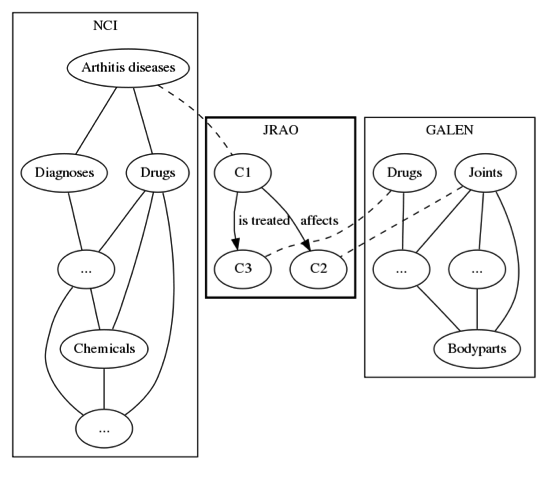
\includegraphics[width=0.6\textwidth]{useCaseOnto3.png}
\caption{JRAO  -- Example for Module Extraction}
\label{JRAO}
\end{center}
\end{figure}

 

\section{Use case Onto-4: Interoperability between closed-world data and open-world metadata}
Data collection has become easier and much more widespread over the years. This data has to be 
assigned a meaning somehow, which occurs traditionally in the  form of metadata annotations. For 
instance, consider geographical datasets derived from satellite data and raw sensor readings. 
Current implementations in, e.g., ecological economics\cite{bagstad_aries_2011} require manual 
annotation of datasets with the information relevant for their processes. While there have been 
attempts to standardize such information\cite{european_comission_inspire_2014}, metadata for 
datasets of simulation results are more difficult to standardize. Moreover, it is 
resource-consuming to link the data to the metadata, to ensure the metadata itself is of good 
quality and consistent, and to actually exploit the metadata when querying the data for data 
analysis. 

The data is usually represented in a database or RDF triple store, which work with a closed world assumption on the dataset, and are not expressive enough to 
incorporate the metadata `background knowledge', such as the conditions for validity of the physical laws in the model of the object of observation. These metadata 
require a more expressive language, such as OWL or Common Logic, which operate under an open-world semantics. However, it is unfeasible to translate the 
whole large dataset into OWL or first-order logic. To `meet in the middle', it is possible to declare bridge rules (i.e., a mapping layer) that can link the metadata to 
the data. This approach can be used for intelligent data analysis that combines the data and metadata through querying the system. It enables the analysis of the 
data on the conceptual layer, instead of users having to learn the SQL/SPARQL query languages and how the data is stored. There are various tools and theories 
to realize this, which is collectively called Ontology-Based Data Access/Management, see also [OBDA].

The languages for representing the metadata or ontology, for representing the bridge rules or mapping assertions, and for representing the data are different yet 
they need to be orchestrated and handled smoothly in the system, be this for data analytics for large enterprises, for formulating policies, or in silico biology in the 
sciences. 

DOL  provides the framework for expressing such bridge rules in a systematic way, maintaining these, and building tools for them. 

\section{Use Case Onto-5: Verification of rules translating Dublin Core into PROV}
The Dublin Core Metadata terms, which have been formalized as an RDF Schema vocabulary, developed initially by the digital library community, are less 
comprehensive but more widely used than PROV (cf. Use Case Onto-1). The rules for translating Dublin Core to the OWL subset of PROV (and, with restrictions, 
vice versa) are not known to yield valid instances of the PROV data model, i.e. they are not known to yield OWL ontologies consistent with respect to the OWL axioms that 
capture part of the PROV data model. This may disrupt systems that would like to reason about the provenance of an entity, and thus the assessment of the 
entity's quality, reliability or trustworthiness.
The Dublin Core to PROV ontology translation%
\footnote{\url{http://www.w3.org/TR/2013/NOTE-prov-dc-20130430/}}
  is expressed partly by a symbol mapping and partly by FOL rules. These FOL rules are implemented by CONSTRUCT patterns in the SPARQL RDF query language.%
\footnote{E.g., \url{http://www.w3.org/TR/2013/NOTE-prov-dc-20130430/\#dct-creator}} 
SPARQL has a formal specification of the evaluation semantics of its algebraic expressions, which is different from the model-theoretic semantics of the OWL and RDFS languages; nevertheless SPARQL CONSTRUCT is a popular and immediately executable syntax for expressing translation rules between ontologies in RDF-based languages in a subset of FOL.
DOL  not only supports the reuse of the existing Dublin Core RDFS and PROV OWL ontologies as modules of a distributed ontology (= OMS network), but it is also able to support the description of the FOL translation rules in a sufficiently expressive ontology language, e.g. Common Logic, and thus enable formal verification of the translation from Dublin Core to PROV.

\section{Use case Spec-1: Specification Refinements}
Especially in safety-critical areas such as medical systems, the automotive industry, avionics and the aerospace industry, but also for microprocessor design, often 
a formal software and hardware development process is used in order to ensure the correct functioning of systems. Typically, a requirement specification is refined 
into a design specification and then an implementation, often involving several intermediate steps (see, e.g. the V-model [V-model], although this does not require 
formal specification).
There are numerous specification formalisms in use, including the OMG's SysML language; moreover, often during development, the formalism needs to be 
changed (e.g. from a specification to a programming language, or from a temporal logic to a state machine). For each of these formalisms, notions of refinement 
have been defined and implemented. However, the lack of a standardized, logically sound language and methodology for such refinement hinders interoperability 
among different development efforts and the reuse of refinements.
DOL  provides the capability to represent refinement that is equally applicable to all DOL-conforming logical languages, and that  
covers at least the most relevant of the industrial use cases of specification refinement.

\section{Use case Spec-2: Modularity of Specifications}
In the context of use case Spec-1, often specifications become so large that it is necessary to structure them in a modular way, both for human readability, 
maintainability, and for more efficient tool support. The lack of a standard for such modular structuring hinders interoperability among different development efforts 
and the reuse of specifications.
DOL  provides a notion of structured modular specification that is equally applicable to all DOL-conforming logical languages.
	
\section{Use case Model-1: Coherent semantics for multi-language models}
\ednote{Isn't this one about ontologies,too?}
	
Often a single problem area within a given domain must be described using several formalisms, due to user community requirements, expressiveness, tool support 
and usage, and so forth. A challenge is that typically the different formalizations are written by different people using different logics, and, thus, their overall 
consistency is hard to maintain.
The need for the use of multiple ontology languages, even within the OMG community, is also reflected by the OMG Ontology Definition Metamodel (ODM), which 
provides a number of syntactic transformations between such languages.
One example is the OMG Date-Time Vocabulary (DTV). DTV has been formulated in different languages, each of which addresses different audiences:
\begin{itemize}
\item	 SBVR: business users
\item 	UML (class diagrams and OCL): software implementers
\item 	OWL: ontology developers and users
\item 	Common Logic: (foundational) ontology developers and users
\end{itemize}
With DOL, one can, e.g.,
\begin{itemize}
\item 	formally relate the different formalizations used for DTV, relate the different formalizations using translations,
\item 	check consistency across the different formalizations (using suitable tools),
\item 	extract sub-modules covering specific aspects, and
\item 	specify the OWL version to be an approximation of the Common Logic version (using a heterogeneous interpretation of OMS).
\end{itemize}
Note that the last point does not specify what information is lost in the approximation. Indeed, DOL provides the means to specify requirements on the approximation, e.g., that it maximally preserves the information. 

\section{Use case Model-2: Consistency among UML diagrams of different types}

A typical UML model involves diagrams of different types. Such UML models may have intrinsic errors because diagrams of different types may specify conflicting 
requirements. Typical questions that arise in this context are, e.g.,

\begin{itemize}
\item whether the multiplicities in a class diagram are consistent with each other
\item wether the attributes and operations in a state machine are
available in a class diagram
\item	  whether the sequential composition of actions in an interaction diagram is justified by an accompanying OCL specification,
\item 	whether cooperating state machines comply with pre-/post-conditions and invariants
\item 	if the behavior prescribed in an interaction diagram is realizable by several state machines cooperating according to a composite structure diagram.
\end{itemize}
Such questions are currently hard to answer in a systematic manner. One method to answer these questions and find such errors is a check for semantic 
consistency. Under some restrictions, the proof of semantic consistency can be (at least partially) performed using model-checking tools like Hugo/RT \cite{HugoRT}. 
Once a formal semantics for the different diagram types has been chosen (see, e.g. \cite{HetUML}), it is possible to use DOL to specify in which 
sense the diagrams need to be consistent, and check this by suitable tools.

\section{Use case Model-3: Refinements between UML diagrams of different types, and their reuse}
A problem is a lack of reusability of refinements: Consider a controller for an elevator, which is specified with a UML protocol state machine, enriched with UML 
sequence diagrams and OCL constraints. Assume further that this model is not directly implemented, but first refined to a UML behavior state machine (which then 
can be automatically or semi-automatically transformed into some implementation using standard UML tools). However, there is no standardized language to 
express, document and maintain the refinement relation itself (UML only allows very simple refinements, namely between state machines). This hinders both the 
reuse of such refinements in different contexts, as well as the interoperability of tools proving such refinements to be correct. DOL  
addresses these problems by providing a standardized notation with formal semantics for such refinements. Refinements expressed in this language could, e.g., be 
parameterized and reused in different contexts.

\section{Conclusion}

In the next sections, we discuss  the metalanguage DOL, its features that enable the support of a variety of formalisms, with syntax, well-defined semantics and model theory. DOL 
distills best practices of modularity and metarelations (such as refinement and alignment) across the three areas of ontology design, formal 
specification, and model-driven development. It provides the ability to specify the basis for formal interoperability even among heterogeneous OMS and OMS networks. DOL enables the solutions of the problems described in the use cases above. It also enables the development of OMS libraries, tools and workflows that 
allow  a better exchange and reuse of OMS. Eventually, this will also lead to better, easier developed and maintained systems based on these OMS.


\chapter{Design Overview}
%
%\ednote{replace this section by saying how we respond to the RFP}
%
%\CLnote[type=todo]{Get rid of formal \should/\shall language (e.g.\ in clause headers: \should/\shall applies to conforming implementations anyway, rather than to this standard itself!) – not necessary in an informative clause. TM: I did this in the clause headings, and for the design part also in the clause texts.}
%
%
This clause is informative. Its purpose is to briefly describe the 
%purposes of the Distributed Ontology, Modeling and Specification Language (DOL) and 
the overall guiding principles and constraints of DOL's syntax and semantics.
%
%\todonote{add somewhere: DOL is a meta language and can be used with OMS languages of any expressiveness. As a Meta-language, DOL provides a framework for combining and relating OMS written in specific OMS languages.
%However, DOL cannot be used for writing new basic OMS.}
%
%\todonote{add ref to annex K}
%
%\section{DOL requirements}\label{c:req:overview}
%
%DOL has been designed and developed with several requirements in mind, all arising from its intended role of enabling OMS interoperability. The use of ``{\should}'' in the rest of clause 5 indicates a desired goal but is not required of DOL (in accordance with Annex H of ISO/IEC Directives -- Part 2).
%
%\CLnote[type=todo]{give quick overview here.  Create clause 5.2 for requirements, and 5.3 for design overview. TM: done}
%
%\subsection{DOL is free, generally applicable, open, and extensible.}\label{c:req:extensible}
%
%DOL \should be
%\begin{description}
%\item[free] This \IS \should be freely available for unrestricted use.
%\item[generally applicable] It \should neither be restricted to OMS in a specific domain, nor to foundational OMS, nor to OMS represented in a specific OMS language, nor to OMS stored in any specific repositories.
%\item[open] It \should support mapping, integrating, and annotating OMS across arbitrary internet locations.  It \should make use of existing open standards wherever suitable.  The criteria for extending DOL (see next item) \should be transparent and explicit.
%\item[extensible] It \should provide a framework into which any existing, and, desirably, any future OMS language can be plugged.
%\end{description}
%
%DOL \shall be applicable to any OMS language that has a formal, logic-based semantics or a semantics defined by translation to another OMS language with such a formal semantics. The annotation framework of DOL \should additionally be applicable to the non-logical constructs of such languages. This \IS \todonote[author=Christoph Lange,date=D:201109221211+02'00',type=fyi]{We can afford to say ``shall'' here, as these criteria are really something that we can fully provide} \shall specify formal criteria for establishing the conformance of an OMS language with DOL.  Annexes \shall establish the conformance of a number of relevant OMS languages with DOL; a registry shall offer the possibility to add further (also non-standardized) languages:\CLnote[date=D:201201100956+01'00']{John Sowa: Make it modular with a simple core that can run efficiently on small systems, but can grow indefinitely to support as much as anyone could desire.}
%
%\begin{description}
%\item[normative] OWL, Common Logic, RDFS\todonote[author=Christoph Lange,date=D:201111021905+01'00']{RIF as well?  See \ticket{16}}
%\item[informative] F-logic,  UML class diagrams, OBO (see appendix~\ref{a:ext-graph} for a longer list)
%\end{description}
%
%\subsection{DOL is a logic-agnostic metalanguage, in the sense that its constructs can be used for many different logics.}\label{c:req:agnostic}
%
%\CLnote{here and elsewhere: remove ``shall'' from section headers}
%
%DOL \shall provide syntactic constructs for structuring OMS regardless of the logic their sentences are formalized in. DOL \should provide syntactic constructs for
%
%\begin{itemize}
%\item basic and structured OMS (and facilities to identify them in a globally unique way),
%\item explicit extraction of modules from existing OMS, \markupcomment[author=Christoph Lange,type=q-aut]{such that, \eg, changes in the OMS can be propagated to the extracted module}{This rather sounds like a use case description to me than like a requirement.  Move it somewhere else?  Where?}.
%\item mappings between OMS (\cf \cref{c:req:links}), including interpretations, relations between OMS and their modules, as well as alignments.
%\end{itemize}
%DOL \shallnot provide its own constructs for expressing sentences.  Instead, it \shall \textit{inherit} the logical language aspects of conforming OMS languages.  It \should be possible to literally include sentences expressed in such OMS languages in a DOL OMS.
%
%DOL \shall provide an initial set of built-in approximation methods and module extraction selectors.  Additionally, it \shall provide a means of referring to approximation methods and module extraction selectors defined externally of this \IS.\todonote[author=Christoph Lange,date=D:201111030047+01'00',type=fyi]{In practice we will use IRIs for that purpose.}
%
%DOL \shall provide an initial vocabulary for expressing relations in correspondences (as part of alignments between OMS).  Additionally, it \shall provide a means of reusing relation types defined externally of this \IS.
%
%DOL \shallnot provide an annotation vocabulary, i.e.\ it \shall neither provide annotation properties nor datatypes to be used with literal annotation objects. Instead, an informative annex \shall recommend existing annotation vocabularies for use with DOL.
%
%\subsection{DOL has user- and machine-readable serializations.}
%
%\CLnote[type=q-all]{We need to revise this following the agreement to drop the XML and RDF serializations.}In the interest of wide applicability and tool support, DOL \should support multiple alternative serializations.  In particular, there \should be a text serialization targeting human readers and writers, as well as serializations optimized for machine processability.
%
%This \IS \shall specify criteria for a serialization to conform with DOL, and it \shall specify the following conforming serializations:
%
%\begin{itemize}
%\item a human-readable \textbf{text serialization}
%\item a machine-processable \textbf{interchange format}, to be implemented as
%  \begin{description}
%  \item[an XML schema (DOL XML)] particularly targeting document or form based authoring, validation, as well as translation from and to serializations of existing OMS languages\todonote[author=Christoph Lange,date=D:201204050853+02'00',type=q-all]{I think it's reasonable to call this ``DOL XML'' instead of ``DIF XML'', as to emphasize the ``brand'' DOL}, and
%  \item[an RDF vocabulary (DOL RDF)] particularly targeting interlinking and annotation.
%  \end{description}
%\end{itemize}
%
%The \textbf{text serialization} in particular \shall offer a syntax for abbreviating identifiers of resources within OMS in a way that does not require authors to write down their full global identifiers.
%
%An OMS implemented in DOL \should be able to comprise parts formalized in any OMS language; any serialization of DOL \should be able to literally include such parts, regardless of the OMS language serialization they have been written in. \todonote[author=Christoph Lange,date=D:201109200256+02'00',type=fyi]{advanced namespacing is the solution that addresses this requirement} Additionally, an OMS implemented in DOL \should be able to refer to any external OMS formalized in any OMS language, as long as they can be identified in a globally unique way.
%
%Existing OMS in existing XML serializations (\eg XCL) or text serializations (\eg OWL Manchester Syntax) \should validate as DOL OMS with a minimum amount of syntactic adaptation. Existing OMS files/documents \should be usable in a DOL context without the need for modification.
%
%\subsection{DOL has a well-defined formal, logic-based semantics.}\label{c:req:semantics}
%
%The structural elements and structural mappings of DOL \should have a formal, logic-based semantics.
%
%This \IS specifies OMS language translations between conforming languages:\todonote[author=Christoph Lange,date=D:201110060000+02'00',type=fyi]{we shall establish the conformance of an initial set of languages with DOL. As a part of that work we deliver the "onto-logical translation graph" between these languages. Anyone, who wants to establish the conformance of another language with DOL, has to add a node to the graph, and at least one edge from/to an existing node.}
%
%\begin{itemize}
%\item OMS language translations between their logical language aspects. For any such OMS language translation its properties \should be determined, \eg whether it is a sublogic, a theoroidal translation, etc. \\
%~\todonote[author=Christoph Lange,date=D:201110060000+02'00',type=todo]{meet the requirements of people who combine OWL reasoners with Prolog. Some additional research needed on combining logics that have a model theory with those that don't}
%\item OMS language translations between their structuring language aspects and the structuring language aspect of DOL.
%\end{itemize}
%DOL can express the application $T(O)$ of an OMS language translation $T\colon L_1\to L_2$ to an OMS $O$ written in langauge $L_1$\todonote[author=Christoph Lange,date=D:201110060000+02'00',type=fyi]{T shall be identified by a IRI. There might be multiple different possible translations between two languages, \eg two ways of expressing OWL roles in CL (binary predicate vs.\ boolean function).  But in order to free the user from always writing down such IRIs, we shall specify some defaults in our translation graph.}, see the abstract syntax category
%\syntax{Translation} in clause~\ref{c:abstract-syntax}.  DOL need not be capable of expressing OMS language translations.
%
%\begin{figure}
%  \centering
%  \documentclass{standalone}
\usepackage[T1]{fontenc}
\usepackage[utf8]{inputenc}
\usepackage{fourier}
\renewcommand{\sfdefault}{Myriad-LF}
\usepackage[scaled=.8]{beramono}
% Minion and Myriad fonts – comment these lines if you don't have them!
% (http://lglinux.blogspot.com/2007/09/myriad-and-minion-for-latex.html)
\usepackage[minionint,mathlf]{MinionPro}
\usepackage{tikz}
\usetikzlibrary{shadows,shapes,positioning,arrows}
\tikzstyle{ontoiop}=[font=\sffamily,
    language/.style={circle,draw},
    translation/.style={-stealth'},
    dol/.style={rectangle,rounded corners,draw,align=left},
    import/.style={-o},
]
% Our colors
\definecolor{cl}{RGB}{127,129,209}
\definecolor{owl}{RGB}{138,173,72}
\definecolor{rdfs}{RGB}{232,146,31}
\definecolor{dol}{RGB}{253,246,234}
\definecolor{owlxml}{RGB}{240,251,239}
\definecolor{clif}{RGB}{242,242,251}

\begin{document}
  \begin{tikzpicture}[ontoiop]
    % Common Logic
    \node[label=Common Logic,language,fill=cl] (cl) {};
    % OWL
    \node[label=below:OWL,language,fill=owl,below left=of cl] (owl) {};
    % RDFS
    \node[label=below:RDFS,language,fill=rdfs,below right=of cl] (rdfs) {};
    \draw[translation] (owl) to (cl);
    \draw[translation] (rdfs) to (cl);
  \end{tikzpicture}
\end{document}

%  \caption{Translating two OMS languages into a third
%one}
%\label{f:DOL-translations}
%\end{figure}
%
%For each pair $L_1$ and $L_2$ of OMS languages, OMS language translations $T_1$ and $T_2$ into a common target OMS language $L_T$ \should be specified. (If $L_T$ does not exist, the only way to express a heterogeneous OMS involving $L_1$ and $L_2$ may be to keep the DOL expression and the individual OMS in $L_1$ and $L_2$.)  These \should be translations into an OMS language that is more expressive than both $L_1$ and $L_2$, such that the union of the images of the translations is a subset of the target OMS language ($T_1(L_1)\cup T_2(L_2)\subseteq L_T$).  \fref{f:DOL-translations} outlines such an example, where Common Logic serves as the common target for OWL and RDFS, as it is more expressive than either of them.\todonote[author=Christoph Lange,date=D:201110060000+02'00',type=fyi]{In the context of that, specify when a document/an OMS conforms with DOL.}  If such a target OMS language or suitable translations do not yet exist, translations into a less expressive language may be specified as an alternative, such that the intersection of the images of the translations forms a subset of the target language ($T_1(L_1)\cap T_2(L_2)\subseteq L_T$), which \should be as large as possible.  For example, an OMS language that is more expressive than both Common Logic and F-Logic does not yet exist; therefore, it would be possible to specify translations into the first-order logic subset of either OMS language.
%
%
%
%Reductions of DOL to conforming OMS languages, as well as approximations of DOL in conforming OMS languages, are specified.  This is to ensure that OMS that have originally been written in DOL can be reused and extended in the respective target OMS languages. While approximations are desirable that preserve as much information from the DOL OMS as the logic underlying the target OMS language is capable of expressing (possibly after a suitable OMS language translation), there \should at least be a trivial reduction that throws away all syntactic constructs of the DOL OMS that are not syntactic constructs in the target OMS language. However, those constructs are optionally preserved as annotations in the output (cf. \cref{c:req:annotation} for annotations).
%
%\todonote[author=Christoph Lange,date=D:201110060000+02'00',type=todo]{provide example of integrating two OMS in a single-sorted logic by translating into many-sorted logic, where only many-sorted logic would guarantee consistency}
%
%\section{DOL design}
\label{c:design:overview}
%
We give an overview of the most important and innovative language
constructs of DOL. Details can be found in clause~\ref{c:abstract-syntax}.


DOL gives interoperability a formal grounding and makes heterogeneous OMS and OMS networks and services based on them amenable to checking of coherence (e.g. consistency, conservativity, intended consequences, and compliance). OMS languages are declarative languages for making ontological distinctions formally precise, for modeling a domain in an unambiguous way, or for expressing algebraic specifications of software.   OMS languages are distinguished by the following features:

\begin{description}
\item[Logic] Most commonly, OMS languages are based on a description logic or some other subset of first-order logic, but in some cases, also higher-order, modal, paraconsistent and other logics are used.
\item[Modularity] A means of structuring an OMS into reusable parts, reusing parts of other OMS, mapping imported symbols to those in the importing OMS, and asserting additional properties about imported symbols.
\item[Annotation] A means of attaching human-readable descriptions to OMS symbols, addressing knowledge engineers and service developers, but also end users of OMS-based services.\ednote{TODO Christoph: reformulate. DOL enables the use of annotations}
\end{description}
Whereas the first feature determines the expressivity of the language and the possibilities for automated reasoning (decidability, tractability, etc.), the latter two intend to facilitate OMS engineering as well as the engineering of OMS-based software.

Acknowledging the wide tool support that conforming established languages such as OWL, Common Logic, MOF, or CASL\ednote{review language list when annexes are finished} enjoy, existing OMS in these languages remain as they are within the DOL framework. DOL enhances their modularity and annotation facilities to a superset of the modularity and annotation facilities they provide themselves. DOL's modularity and annotation constructs can either be embedded into existing OMS as non-disruptive annotations, or they can be provided as standoff markup, pointing to the OMS they talk about; DOL specifies a syntax and semantics for both variants. DOL's modularity constructs are semantically well-founded within a library of formal relationships between the logics underlying the different supported OMS languages.


\section{Overview of DOL}\label{c:req:overview}
\ednote{TM: rewrite}

DOL is a language enabling OMS interoperability. 
DOL is
\begin{description}
\item[free] DOL is freely available for unrestricted use.
\item[generally applicable] DOL is neither be restricted to OMS in a specific domain, nor to foundational OMS, nor to OMS represented in a specific OMS language, nor to OMS stored in any specific repositories.
\item[open] DOL supports mapping, integrating, and annotating OMS across arbitrary internet locations.  It makes use of existing open standards wherever suitable.  The criteria for extending DOL (see next item) are transparent and explicit.
\item[extensible] DOL provides a framework into which any existing, and, desirably, any future OMS language can be plugged.
\end{description}
DOL is applicable to any OMS language that has a formal, logic-based semantics or a semantics defined by translation to another OMS language with such a formal semantics. The annotation framework of DOL is additionally applicable to the non-logical constructs of such languages. This \IS specifies formal criteria for establishing the conformance of an OMS language with DOL.  Annexes establish the conformance of a number of relevant OMS languages with DOL; a registry shall offer the possibility to add further (also non-standardized) languages:\CLnote[date=D:201201100956+01'00']{John Sowa: Make it modular with a simple core that can run efficiently on small systems, but can grow indefinitely to support as much as anyone could desire.}
DOL provides syntactic constructs for structuring OMS regardless of the logic their sentences are formalized in. 
DOL does not provide its own constructs for expressing sentences.  Instead, it \textit{inherits} the logical language aspects of conforming OMS languages.  It is possible to literally include sentences expressed in such OMS languages in a DOL OMS.
DOL provides an initial vocabulary for expressing relations in correspondences (as part of alignments between OMS).  Additionally, it provides a means of reusing relation types defined externally of this \IS.
DOL does not provide an annotation vocabulary, i.e.\ it neither provides annotation properties nor datatypes to be used with literal annotation objects. Instead, an informative annex recommends existing annotation vocabularies for use with DOL.
\CLnote[type=q-all]{We need to revise this following the agreement to drop the XML and RDF serializations.}In the interest of wide applicability and tool support, DOL  supports multiple alternative serializations.  In particular, there is a text serialization targeting human readers and writers, as well as serializations optimized for machine processability.
The \textbf{text serialization} in particular offers a syntax for abbreviating identifiers of resources within OMS in a way that does not require authors to write down their full global identifiers.
An OMS implemented in DOL can comprise parts formalized in any OMS language; any serialization of DOL can literally include such parts, regardless of the OMS language serialization they have been written in. \todonote[author=Christoph Lange,date=D:201109200256+02'00',type=fyi]{advanced namespacing is the solution that addresses this requirement} Additionally, an OMS implemented in DOL can refer to any external OMS formalized in any OMS language, as long as they can be identified in a globally unique way.
Existing OMS in existing XML serializations (\eg XCL) or text serializations (\eg OWL Manchester Syntax) validate as DOL OMS with a minimum amount of syntactic adaptation. Existing OMS files/documents are usable in a DOL context without the need for modification.


DOL does not provide a new elementary OMS language, but provides a
layer to be used on top of existing elementary OMS languages which
enables OMS engineers to formally express mappings between OMS written
in different languages and stored at different Web locations. The
purpose of such OMS networks is enabling a greater extent of
interoperability between data and services in complex application
settings.


The following features are essential to the design of this \IS:

\begin{itemize}
\item DOL is a language covering OMS modularity, OMS heterogeneity, and
OMS mapping. In particular, it enables writing structured OMS
(thereby reusing existing OMS), OMS involving different languages,
as well as complex mappings and relations between OMS.
\item DOL is a declarative language with a formal semantics.
% for modular OMS that consist of structured OMS that are possibly heterogeneous, i.e.\ are written within the same or in different OMS languages, and made available at different Web locations.
\item DOL provides a superset of the modularization, Web awareness and annotation facilities of a number of commonly used OMS languages, including OWL \cite{OWL2}, RDF \cite{RDF}, Common Logic \cite{ISO/IEC 24707:2007} and UML \cite{UML}.\footnote{See \cref{c:req:extensible} for details.}
\item DOL is an open, extensible standard that is not restricted to a fixed set of supported OMS language but specifies criteria for any existing or future OMS language to conform with DOL.
\item Existing OMS in languages conforming with DOL remain as they are; they can be enriched with DOL's modularity and annotation constructs in a non-disruptive way.
\end{itemize}

\ednote{reformulate this, see RFP}



\section{DOL enables expression of logically heterogeneous OMS and literal reuse of existing OMS.}
DOL is a mechanism for expressing logically heterogeneous OMS. It can be used to combine sentences and structured OMS expressed in different conforming OMS languages
and logics into single documents or modules. With DOL, sentences or structured OMS of previously existing OMS in
conforming languages can be reused by literally including them into a DOL OMS. A minimum of wrapping constructs and other annotations (e.g., for identifying the language of a sentence) are provided. 
\todonote[author=Christoph
Lange,date=D:201109201457+02'00',type=todo]{Figure out what this
  feedback item from Michael Grüninger (?) means: say that there
  should be a syntax for relationships btw. OMS as well as a
  syntax for heterogeneous OMS. (If you write down an OMS,
  it might involve constructs that only exist in OWL)} See the
abstract syntax category \syntax{OMS} in
clause~\ref{c:abstract-syntax}.

\section{DOL includes provisions for expressing mappings between OMS.}\label{c:req:links}

DOL provides a syntax for expressing mappings between OMS -- logical OMS Mappings as well as alignments.  One use case illustrating both is sketched in  \fref{f:DOL-mapping}. This \IS defines a set of logical OMS mapping types and a set of non-logical OMS mapping types.

Logical OMS mappings supported by DOL include:
\begin{itemize}
\item imports (particularly including imports that lead to conservative extensions), see the
abstract syntax categories \syntax{OMSRef} and \syntax{ExtensionOMS} in
clause~\ref{c:abstract-syntax}.
\item interpretations (both between focused OMS and OMS networks), see the
abstract syntax category \syntax{IntprDefn} in
clause~\ref{c:abstract-syntax}.
\item mappings between OMS and their modules, see the
abstract syntax category \syntax{ModuleRelDefn} in
clause~\ref{c:abstract-syntax}.
\end{itemize}
DOL allows such links to express signature translations in such OMS mappings; see the
abstract syntax category \syntax{SymbolMapItems} in
clause~\ref{c:abstract-syntax}.

DOL need not be able to fully represent logical translations but is
capable of referring to them.

\todonote[author=Christoph Lange,date=D:201111231324+01'00',type=q-aut]{We had this comment here; what does it mean?  ``DOL only maps symbols to expressions''}

DOL can also be used to combine or merge OMS along such OMS mappings, see
the rule for \syntax{combination} for the abstract syntax category
\syntax{OMS} in clause~\ref{c:abstract-syntax}.

\begin{figure}
  \centering
  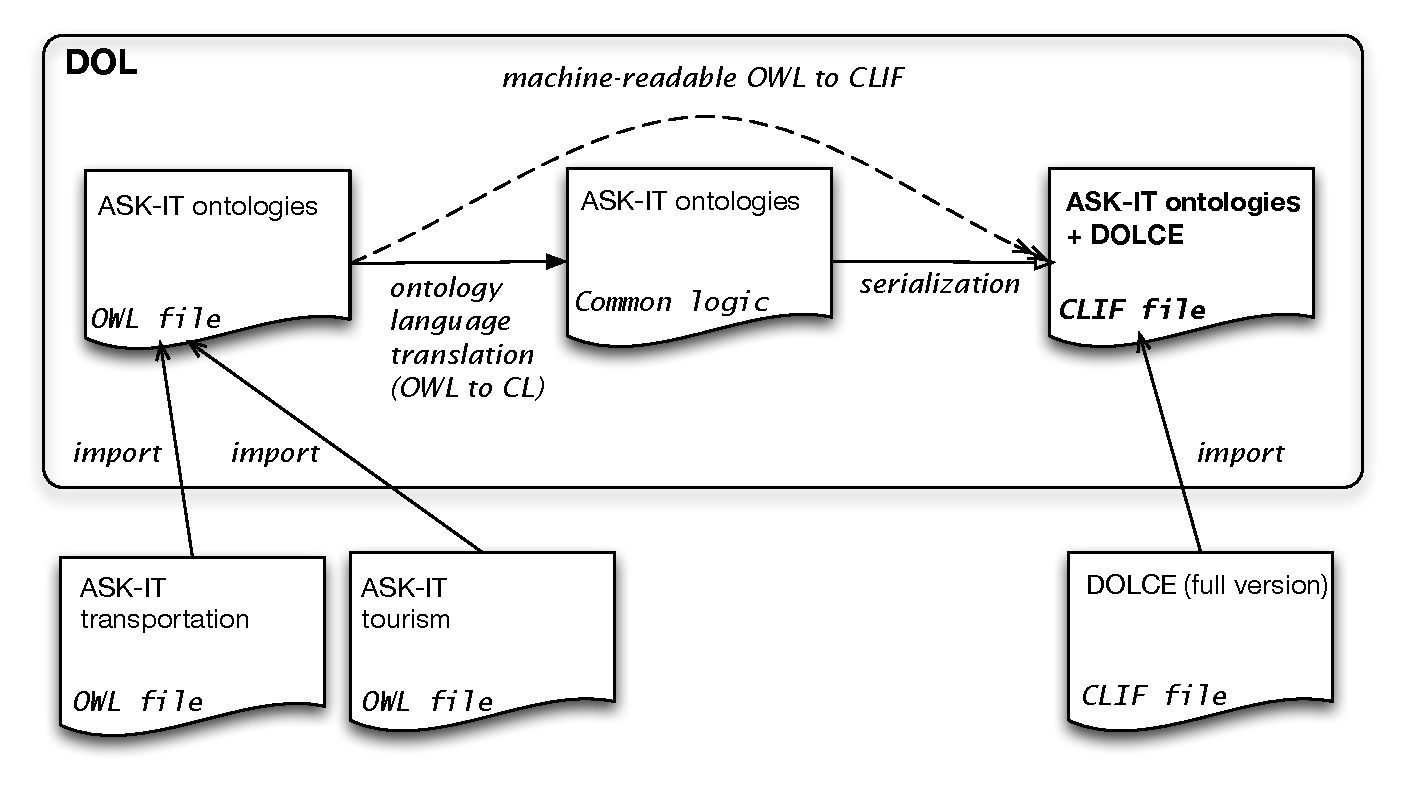
\includegraphics[width=\textwidth]{illustrations/DOLfig.pdf}
  \caption{Mapping between two OMS formulated in different OMS languages}
\label{f:DOL-mapping}
\end{figure}

\section{DOL enables the representation of OMS and OMS mappings at different levels of detail}\label{c:explicit}

OMS and OMS mappings expressed in DOL can be based on a
number of implicit assumptions about which OMS language
translation or which ontology matcher has been employed.  Depending on
the OMS engineering workflow or application setting, it can be
useful to keep these assumptions implicit or to make them explicit.
DOL allows such assumptions to remain implicit, if desired.
However, it also enables the user to 
capture these assumptions explicitly as annotations
to the OMS.  This \IS specifies a
translation that expands any DOL OMS with implicit assumptions
into its explicit counterpart.\todo{Terry: (Is this true? if so, rewrite). Perhaps:  This OMS Specification provides a means to specify a translation to expand any DOL OMS with implicit assumptions into an  explicit counterpart. 
(is such a translation counterpart necessarily unique, either syntactically or semantically?  If a semantically preserving syntax change occurs to the original, will the counterpart change?)}

The following list covers the possible cases where DOL provides a choice between representing information implicitly or  explicitly:
\begin{description}
\item[default OMS language translations] A heterogeneous OMS can import several (focused) OMS expressed in different conforming logics, for which suitable translations have been defined in the logic graph provided in \aref{a:graph} or in an extension to it that has been provided when establishing the conformance of some other logic with DOL.  Determining the semantics of the heterogeneous OMS requires a translation into a common target language to be applied (\cf \cref{c:semantics}).  This translation is determined via a lookup in the transitive closure of the logic graph.  Depending on the reasoners available in the given application setting, it can, however, be necessary to employ a different translation.  Authors can express which one to employ.  In a multi-step translation, it is possible to implicitly apply as many default translations as possible, and to concentrate on making explicit only those translations that deviate from the default.\CLnote[type=q-aut]{Will this situation be the same for default approximations, or to we need to add an extra item to the list?}
\item[different matching algorithms] OMS alignments, which DOL is able to express, may have been obtained by running different OMS matching algorithms.  If, in a given OMS engineering workflow, the information on which algorithm has been applied is clear from the context, it is possible to omit it in the alignment expressed in DOL.  Otherwise, \eg if the next person working on the OMS requires that information, it is possible to make it explicit.\todonote{TM: the alignment itself should be there explicitly. right? But then the information about the matching algorithm that has produced it is a mere annotation without semantics, isn't it?\\ CL: I agree with you. OK, so we will replace this with approximation algorithms.}
\end{description}

~\todonote[author=Christoph Lange,date=D:201110060000+02'00',type=todo]{ask Michael Gr{\"u}ninger for his mereology example in CL}

\section{DOL provides a mechanism for rich annotation and documentation of OMS.}\label{c:req:annotation}

\todonote[author=Christoph Lange,date=D:201211141640+00'00',type=q-all]{I think that now that we have agreed on dumping the RDF and XML serializations of DOL, this requirement can no longer be satisfied.  Or maybe it can be satisfied in a trivial way (nonetheless requiring this section to be shortened): DOL provides the mechanism for  identifying anything of relevance in a library, it will do so by IRIs, and with RDF there is an established mechanism for annotating things identified by IRIs.  Still I believe this requirement is an important selling point.} DOL supports  annotations in the full generality specified in \cref{c:terms-annotation}.  The DOL serializations further support the fine-grained embedding of annotations into OMS. % up to the granularity of literate programming.

The DOL serializations also supports the annotation of existing OMS via non-intrusive standoff markup, which points to the annotation subjects from external documentation files or from special embedded comments, extending the comment syntax of the respective OMS language; for XML serializations of OMS languages, RDFa extensions are specified, so that DOL RDF can be embedded.

A list of RDF vocabularies for annotating OMS is recommended as an annex to this \IS.


\clause{DOL abstract syntax}\label{c:abstract-syntax}

\sclause{Abstract syntax categories}

DOL provides abstract syntax categories for
\begin{itemize}
\item libraries (items in libraries are: OMS definitions, OMS mapping definitions, queries, and qualifications choosing the logic,
OMS language and/or serialization)
\item \red{focused OMS} (which can be basic OMS in some
OMS language, or unions, translations, minimizations, combinations,
approximations of OMS, among others)
\item OMS mappings 
\item \red{queries}
\item identifiers
\item annotations
\end{itemize}
 
Additionally, the categories of the abstract syntaxes of any conforming OMS languages (\cf \cref{c:conform:logic}) are also DOL abstract syntax categories.

The following subclauses, one per abstract syntax category, specify the abstract syntax of DOL in EBNF. Note that we deviate from the EBNF specification in
 \nisref{ISO/IEC 14977:1996} in favor of a more modern and concise
EBNF syntax.\footnote{\red{More precisely, \nisref{ISO/IEC 14977:1996} requires commas between the (non-)terminals of a right-hand side, which we omit 
for the sake of better readability. Also, we replace the separator \syntax{=}
between left and right hand-side of a rule with \syntax{::=}, and 
use the notation \syntax{N+}
of one or more repetitions of \syntax{N}.}}  
%Note that ISO EBNF lacks an operator for ``at least one repetition''.  This \IS therefore adopts the following convention: Whenever some sequence \syntax{S} is repeated at least once, we give it a non-terminal identifier of its own (\syntax{RepeatedS = S \{ S \} ;}), or group it as in \syntax{LongerExpression = Foo Bar ( S \{ S \} ) ;}.

\sclause{Libraries}\label{c:libraries}

A library (\syntax{Library}) consists of a collection of (named) focused OMS and mappings between these.  More specifically, a
library consists of a name, followed by a list of
\syntax{LibraryItem}s.  A \syntax{LibraryItem} is either a
definition of a focused OMS  (\syntax{OMSDefn}), 
\red{a definition of a library  (\syntax{LibraryDefn}),}
a mapping between OMS
(\syntax{MappingDefn}), a definition related to queries 
(\syntax{QueryRelatedDefn})
or a \syntax{Qualification} selecting a specific
OMS language, logic and/or syntax that is used to interpret the
subsequent \syntax{LibraryItem}s.  Alternatively, a library can also be the verbatim inclusion of an OMS written in
an OMS language that conforms with DOL (\syntax{OMSInConformingLanguage}; \cf \ref{c:conform:logic}).

\begin{lstlisting}[language=ebnf,escapeinside={()}]  % abstract syntax
Library                  = [ PrefixMap ] , LibraryDefn
                         | OMSInConformingLanguage ;
LibraryDefn              = 'library' , LibraryName , { LibraryItem } ;
OMSInConformingLanguage  = ($<$)language specific($>$) ;
LibraryItem              = LibImport | OMSDefn | NetworkDefn | MappingDefn | QueryRelatedDefn | Qualification ;
LibImport                = 'lib-import' , LibraryName ;
Qualification            = LanguageQual | LogicQual | SyntaxQual ;
LanguageQual             = 'lang-select' , LanguageRef ;
LogicQual                = 'logic-select' , LogicRef ;
SyntaxQual               = 'syntax-select' , SyntaxRef ;
LibraryName              = IRI ;
\end{lstlisting}
~\todonote[type=fyi,author=Christoph Lange]{Things changed from HetCASL:\textLF
  • logic-select now mandatory (no default logic) and tree-scoped MC: what does this mean? To make Hets-lib conform with this, we should have .het files equivalent to .dol files with logic selected to be CASL\textLF
  • download-items (encourage linked data best practices instead)\textLF
  • item-name-map (to be replaced by namespaces??)\textLF
  • lib-version (to be replaced by metadata annotations, \eg OMV)\textLF
  • indirect-mapping (will always use full IRIs, and abbreviate them by syntactic namespaces)}

At the beginning of a library, one can declare a \syntax{PrefixMap} for abbreviating long IRIs; see \cref{c:identifiers} for details.

\red{
Inside a library, one can defined OMS networks (\syntax{NetworkDefn}).
A \syntax{NetworkDefn} names an
OMS network consisting of focused OMS and OMS mappings. OMS networks may build on previously-defined
OMS networks, and they can be used in \syntax{combination}s.  
}
\begin{lstlisting}[language=ebnf,escapeinside={()}]  % abstract syntax

NetworkDefn            = 'network-defn', NetworkName , [ ConsStrength ] , Network ;
NetworkName            = IRI ;
Network                = 'network', NetworkElements , ExcludeExtensions ;
NetworkElements        = 'network-elements' , { NetworkElement } ;
NetworkElement         = 'network-element' , [ Id ] , OMSOrMappingorNetworkRef ;
ExcludeExtensions    = 'exclude-imports' , { OMSOrMappingorNetworkRef } ; 
OMSOrMappingorNetworkRef  = IRI ;
\end{lstlisting}


\sclause{Focused OMS}

A focused OMS (\syntax{OMS}) can be one of the following:
\begin{itemize}
\item a basic OMS \syntax{BasicOMS} written inline, in a conforming serialization of a conforming OMS 
language\footnote{In this place, any OMS in a conforming serialization of a conforming OMS language is permitted.  
However, DOL's module sublanguage should be given preference over the module sublanguage of 
the respective conforming OMS language; \eg DOL's extension construct should be preferred over OWL's import construct.},
\item a translation of an OMS into a different signature or OMS
language,
\item a reduction of an OMS to a smaller signature and/or less
expressive logic (that is,
some non-logical symbols are hidden, but the semantic effect of sentences involving these is kept),
\item a module extracted from an OMS, using a restriction signature,
\item an approximation of an OMS, in a subsignature or sublogic, with the effect that sentences not expressible in the subsignature resp.\ sublogic are replaced with a suitable approximation,
\item \red{a filtering of an OMS, with the effect that some signature symbols and axioms are removed from the OMS,}
\item a union of several OMS,
\item an extension of an OMS with a basic or a minimizable OMS, optionally named and/or marked as conservative, monomorphic, definitional or implied,
\item a reference to an OMS existing on the Web,
\item an OMS qualified with the OMS language that is used to express it,
\item a combination of OMS (technically, this is a colimit, see \cite{ZimmermanEtAl06}),\footnote{A combination of OMS also takes all mappings into these OMS into consideration---unless these are explicitly excluded.}
\item a minimization of an OMS, forcing the subsequently declared
  non-logical symbols to be interpreted in a minimal way, while the non-logical symbols declared so far are fixed (alternatively, the non-logical symbols to be minimized and to be varied can be explicitly declared). \red{Variants are
maximization, freeness (minimizing also data sets and equalities on these), and cofreeness
(maximizing also data sets and equalities on these),}
\item \red{the application of a substitution to a sentence.}

\end{itemize}
% derived from CASL (see CASL reference manual)
% and HetCASL (see HetCASL summary)

\begin{lstlisting}[language=ebnf,escapeinside={<>}]  % abstract syntax
BasicOMS             = OMSInConformingLanguage ;
MinimizableOMS       = BasicOMS
                     | 'oms-ref' , OMSRef , [ ImportName ] ;
ExtendingOMS         = MinimizableOMS
                     | 'minimize' , MinimizableOMS ;
OMS                  = ExtendingOMS
                     | 'minimize-symbols' , OMS , Minimization
                     | 'translation' , OMS , Translation
                     | 'reduction' , OMS , Reduction
                     | 'module-extract' , OMS , Extraction 
                     | 'approximation' , OMS , Approximation
                     | 'filtering', OMS, Filtering
                     | 'union' , OMS , [ ConsStrength ] , OMS 
                     | 'extension' , OMS , ExtensionOMS
                     | 'qual-oms' , { Qualification } , OMS
                     | 'bridge' , OMS, { Translation } , OMS
                     | 'combination' , Network
                     | 'application', SubstName, Sentence ;

Minimization         = MinType, CircMin , CircVars ;
MinType              = 'minimize' | 'maximize' | 'free' | 'cofree' ;
CircMin              = Symbol , { Symbol } ;
CircVars             = { Symbol } ;

Translation          = 'renaming' , { LogicTranslation } , [ SymbolMapItems ] ;
LogicTranslation     = 'logic-translation' , OMSLangTrans ;

Reduction            = 'hidden' , { LogicReduction } , [ SymbolItems ]
                     | 'revealed' , SymbolMapItems  ;
LogicReduction       = 'logic-reduction' , OMSLangTrans ;

SymbolItems          = 'symbol-items' , ( Symbol , { Symbol } ) ;
SymbolMapItems       = 'symbol-map-items' , ( SymbolOrMap , { SymbolOrMap } ) ;

Extraction           = 'extraction', [ QualInterfaceSignature ] ;

Approximation        = 'approximation' , QualInterfaceSignature , [ LogicRef ] ;

Filtering            = 'select' , BasicOMS 
                     | 'reject' , BasicOMS ;

ExtensionOMS         = [ ExtConsStrength ] , [ ExtensionName ] , ExtendingOMS ;

ConsStrength         = Conservative | 'monomorphic'
                     | 'weak-definitional' | 'definitional' ;

ExtConsStrength      = ConsStrength | 'implied' ;

Conservative         = 'consequence-conservative' | 'model-conservative' ;

QualInterfaceSignature   = 'keep-signature' , InterfaceSignature 
                         | 'remove-signature' , InterfaceSignature ;

InterfaceSignature   = SymbolItems ;
ImportName           = IRI ;
ExtensionName        = IRI ;
\end{lstlisting}
%% \ednote{Alternatively, we could use one type of \syntax{InterfaceSignature}
%% only, and instead use different constructors for \syntax{Extraction}
%% and \syntax{Approximation}. This would be a bit more verbose, but a bit
%% more coherent with position of non-terminals in the concrete syntax.}

An OMS definition \syntax{OMSDefn} names a focused OMS.  

It can be
optionally marked as consistent, monomorphic or having a unique model using 
\syntax{ConsStrength}.\footnote{More precisely, \syntax{'consequence-conservative'}
here requires the OMS to have a non-trivial set of logical consequences, while \syntax{'model-conservative'}
requires its satisfiability. \syntax{'definitional'} expresses the unique model property; this may be interesting for 
OMS (e.g.\ returned by model finders) that are used to describe single models.}. An
\syntax{SymbolItems}, used in an OMS \syntax{Reduction}, is a
list of non-logical symbols that are to be hidden. A \syntax{LogicReduction}
denotes a logic reduction to a
less expressive OMS language. A \syntax{SymbolMapItems}, used in
OMS \syntax{Translation}s,  maps symbols to symbols\CLnote[type=fyi]{On 2012-07-18 we decided 
not to specify lambda-style symbol-to-term mappings for now.  Would be convenient, but specifying its semantics 
in an OMS language independent way would require additional institution infrastructure – and the same effect can be 
achieved by auxiliary definitional extensions, cf.\ Colore (so promote this, informatively, as a ``best practice''?) TM: Alternatively, we could use a recent notion of institutional monad. This builds an extended signature with all terms. Then one can use ordinary signature morphisms into such extended signatures.}, or a logic
translation. An OMS language translation \syntax{OMSLangTrans} 
can be either specified by its name, or be inferred as the default
translation between to a given target (the source will be inferred as the 
OMS language of the current OMS).

\begin{lstlisting}[language=ebnf,escapeinside={()}]  % abstract syntax
OMSDefn          = 'oms-defn' , OMSName , [ ConsStrength ] , OMS ;
Symbol           = IRI ;
SymbolMap        = 'symbol-map' , Symbol , Symbol ;
SymbolOrMap      = Symbol | SymbolMap ;
Term             = ($<$)an expression specific to a basic OMS language($>$) ;
Sentence         = ($<$)an expression specific to a basic OMS language($>$) ;
                 
OMSName          = IRI ;
                 
OMSRef           = IRI ;
ExtensionRef     = IRI ;
                 
LoLaRef          = LanguageRef | LogicRef ;
                 
LanguageRef      = IRI ;
LogicRef         = IRI ;
SyntaxRef        = IRI ;
                 
OMSLangTrans     = 'named-trans' , OMSLangTransRef
                 | 'default-trans' , LoLaRef ; 
                 
OMSLangTransRef  = IRI ;
                 
\end{lstlisting}


\sclause{OMS Mappings}

A OMS mapping provides a connection between two OMS. A OMS mapping definition is the definition of 
either a named interpretation (\syntax{IntprDefn}, \red{\syntax{Entailment}} or 
\syntax{EquivDefn}), a named declaration of the  relation between a module of an OMS and the whole 
OMS (\syntax{ModuleRelDefn}), or a named alignment (\syntax{AlignDefn}).

The \syntax{SymbolMapItems} in an interpretation always must lead to a signature morphism; a proof 
obligation expressing that the (translated) source OMS logically follows from the target OMS is 
generated.  \red{An entailment is a variant where all symbols are mapped identically, while an 
equivalence states that the model classes of two OMS are in bijective correspondence.}

\red{
Interpretations, entailments and equivalences between OMS networks are also possible. An 
interpretation between OMS networks has to specify both a mapping between the nodes of the OMS 
network, as well as, for each node, a symbol map from the OMS of that node to the target OMS to 
which it is mapped.
%\ednote{In equivalences between OMS networks, should we allow for node mappings 
%as well? In  \cite{MossakowskiTarlecki09}, this is allowed.
%--- No, since we do not allow for signature morphisms either.}
}

In contrast to this functional style of mapping symbols, an alignment provides a relational 
connection between two OMS,  using a set of \syntax{Correspondence}s. Each correspondence may relate 
some OMS non-logical symbol to another one (possibly given by a term) with an optional confidence 
value. Moreover, the relation between the two non-logical symbols can be explicitly
specified (like being equal, or only being subsumed) in a similar way to the Alignment API \cite{AlignmentAPI}. 
\red{The relations that can be used in a correspondence are equivalence, disjointness, subsumption, membership (the last two with a
variant for each direction) or a user-defined relation that is stored in a registry and must be prefixed with
\url{purl.net/DOL}.
A default correspondence can be used; it is applied to all pairs of non-logical symbols with 
the same local names. The default relation in a correspondence is equivalence, unless  a different 
relation is specified in a surrounding 
'CorrespondenceBlock'.
Using an \syntax{AlignCard}, left and right injectivity and totality of the
alignment can be specified (the default is left-injective, right-injective, left-total  and right-total).
With \syntax{AlignSem}, different styles of networks of aligned ontologies (to be interpreted in 
a logic-specific way) of alignments can be specified (whether a single domain is assumed, all domains are embedded into a global domain,
or whether several local domains are linked (``contextualized'') by relations).}

A \syntax{ModuleRelDefn} declares that a certain OMS
actually is a module of some other OMS with respect
to the \syntax{InterfaceSignature}.


\begin{lstlisting}[language=ebnf,escapeinside={<>},mathescape]  % abstract syntax
MappingDefn          = IntprDefn | Entailment | EquivDefn | ModuleRelDefn | AlignDefn;

IntprDefn            = 'intpr-defn' , IntprName , [ Conservative ] , 
                        IntprType , { LogicTranslation } , [ SymbolMapItems ]                     
                     | 'refinement' , IntprName , Refinement ;
IntprName            = IRI ;
IntprType            = 'intpr-type' , OMS , OMS ;

Refinement           = 'ref-oms' , OMS 
                     | 'ref-network' , Network
                     | 'ref-composition' , Refinement , Refinement
                     | 'simple-ref' , OMS , RefMap , Refinement ;
RefMap               = 'refmap-oms' ,  { LogicTranslation } , [ SymbolMapItems ] 
                     | 'refmap-network' , { NodeMap } ;
NodeMap              = 'node-map', OMSName , OMSName , { LogicTranslation } , [ SymbolMapItems ] ;


Entailment           = 'entailment' , EntailmentName , EntailmentType ;
EntailmentType       = 'oms-oms-entailment', OMS , OMS 
                     | 'network-oms-entailment', Network , OMS 
                     | 'network-network-entailment', Network, Network ;
EntailmentName       = IRI ;

EquivDefn            = 'equiv-defn' , EquivName , EquivType ;
EquivName            = IRI ;
EquivType            = 'oms-equiv' , OMS , OMS , OMS
                     | 'network-equiv' , Network , Network , Network ;

ModuleRelDefn        = 'module-defn' , ModuleName , [ Conservative ] , ModuleType ,
                                       InterfaceSignature ;
ModuleName           = IRI ;
ModuleType           = 'module-type' , OMS , OMS ;

AlignDefn            = 'align-defn' , AlignName , [ AlignCard ] , AlignType, 
                                    AlignSem,   { Correspondence } ; <\footnote{Note that this grammar uses ``type'' as in ``the type of a function'', whereas the Alignment API uses ``type'' for the totality/injectivity of the relation/function.  For the latter, this grammar uses ``cardinality''.}>
AlignName            = IRI ;
AlignCards           = AlignCardForward , AlignCardBackward ; 
AlignCardForward     = 'align-card-forward' , AlignCard ;
AlignCardBackward    = 'align-card-backward' , AlignCard ;
AlignCard            = 'injective-and-total'
                     | 'injective'
                     | 'total'
                     | 'neither-injective-nor-total' ;
AlignType            = 'align-type' , OMS , OMS ;
AlignSem            = 'single-domain' 
                    | 'global-domain' 
                    | 'contextualized-domain' ; 

Correspondence       = CorrespondenceBlock
                     | SingleCorrespondence
                     | 'default-correspondence' ; 

CorrespondenceBlock  = 'correspondence-block' , [ RelationRef ] , [ Confidence ],
                                                Correspondence, { Correspondence } ; 
SingleCorrespondence = 'correspondence' , SymbolRef , [ RelationRef ] , [ Confidence ] ,
                                          TermOrSymbolRef , [ CorrespondenceID ] ;
CorrespondenceID     = IRI ;
SymbolRef            = IRI ;
TermOrSymbolRef      = Term | SymbolRef ;
RelationRef          = 'subsumes' | 'is-subsumed' | 'equivalent' | 'incompatible' 
                     | 'has-instance' | 'instance-of' | 'default-relation' | IRI ; 
Confidence           = Double ;
\end{lstlisting}
\begin{lstlisting}[language=ebnf,escapeinside={()},mathescape]  % abstract syntax
Double               = ($<$ a number $\in [0,1]$ $>$) ;
\end{lstlisting}

A symbol map in an interpretation is \required to cover all non-logical symbols of the source OMS; 
the semantics specification in \cref{c:semantics} makes this assumption\footnote{Mapping a 
non-logical symbol twice is an error. Mapping two source non-logical symbols to the same target 
non-logical symbol is legal, this then is a non-injective OMS mapping.}.  Applications \shall 
implicitly map those non-logical symbols of the source OMS, for which an explicit mapping is not 
given, to non-logical symbols of the same (local) name in the target OMS, wherever this is uniquely 
defined – in detail:

\begin{algorithmic}
  \REQUIRE $O_s, O_t$ are OMS
  \REQUIRE $M\subseteq\Sigma(O_s)\times\Sigma(O_t)$ maps non-logical symbols (\ie elements of the signature) of $O_s$ to non-logical symbols of $O_t$
  \FORALL{$e_s\in\Sigma(O_s)$ not covered by $M$}
    \STATE $n_s\leftarrow\operatorname{localname}(e_s)$
    \STATE $N_t\leftarrow\{\operatorname{localname}(e)|e\in\Sigma(O_t)\}$
    \IF[\ie if there is a unique target]{$N_t = \{ e_t \}$}
      \STATE $M\leftarrow M\cup\{(e_s, e_t)\}$
    \ENDIF
  \ENDFOR
  \ENSURE $M$ completely covers $\Sigma(O_s)$
\end{algorithmic}

The local name of a non-logical symbol is determined as follows\footnote{In practice, this can 
often have the effect of undoing an IRI abbreviation mechanism that was used when writing the 
respective OMS (\cf \cref{c:identifiers}).  In general, however, functions that turn abbreviations 
into IRIs are not invertible.  For this reason, the implicit mapping of non-logical symbols is 
specified independently from IRI abbreviation mechanisms possibly employed in the 
OMS.}:\hspace{-2cm}
\begin{algorithmic}
  \REQUIRE $e$ is a non-logical symbol (identified by an IRI; \cf \cref{c:identifiers})
  \IF[production \syntax{ifragment} in \nisref{IETF/RFC 3987:2005}]{$e$ has a fragment $f$}
    \RETURN $f$
  \ELSE
    \STATE $n\leftarrow$ the longest suffix of $e$ that matches the \syntax{Nmtoken} production of XML \nisref{W3C/TR REC-xml:2008}
    \RETURN $n$
  \ENDIF
\end{algorithmic}

%Alignments 

\sclause{Queries}
\red{
Queries are a means to extract information from an OMS.  DOL' \syntax{QueryDefn}s cover 
``select''-type queries that deliver an answer substitution for the query variables. (Answer) 
substitutions can be stored separately, using a \syntax{SubstDefn}. A
\syntax{ResultDefn} expresses that certain answer substitutions are
the result of a query. Optioally, a result can be expressed to be
complete, meaning that it comprises all answer substitutions to the query.
}
\begin{lstlisting}[language=ebnf,escapeinside={<>},mathescape]  % abstract syntax
QueryRelatedDefn     = QueryDefn | SubstDefn | ResultDefn ;
QueryDefn            = 'select-query-defn', QueryName, Vars, Sentence, 
                                            OMS, [Translation] ;
SubstDefn            = 'subst-defn', SubstName, OMS, OMS, SymbolMap ;
ResultDefn           = 'result-def', ResultName, SubstName, { SubstName }, 
                                     QueryName, [ Complete ] ;
QueryName            = IRI ;
SubstName            = IRI ;
ResultName           = IRI ;
Vars                 = { Symbol } ;
Complete             = 'complete' ;
\end{lstlisting}

%%%%%%%%%%%%%%%%%%%%%%%%%%%%%%%%%%%%%%%%%%%%%%%%%%%%%%%%%%%%%%%%%%%%%%%%

~\CLnote{some text that was left over here, but I don't recall what we meant by it: recommendations for dealing with OMS language dialects}

\sclause{Identifiers}\label{c:identifiers}

This section specifies the abstract syntax of identifiers of DOL OMS and their elements.

\ssclause{IRIs}\label{c:iris}

In accordance with best practices for publishing OMS on the Web, identifiers of OMS and their 
elements \should not just serve as \emph{names}, but also as \emph{locators}, which, when 
dereferenced, give access to a concrete representation of an OMS or one of its elements.  (For the 
specific case of RDFS and OWL OMS, these best practices are documented in 
\cite{W3C:NOTE-swbp-vocab-pub-20080828}.  The latter is a specialization of the linked data 
principles, which apply to any machine-processable data published on the Web 
\cite{BernersLee:LinkedData2006}.)  It is recommended that publicly accessible DOL OMS be published 
as linked data.

\todonote[type=q-aut,author=Christoph Lange]{Does this motivation/justification sound reasonable to 
you?}Therefore, in order to impose fewer conformance requirements on applications, DOL commits to 
using IRIs for identification \nisref{IETF/RFC 3987:2005}.  It is \recommended that libraries use 
IRIs that translate to URLs when applying the algorithm for mapping IRIs to URIs specified in 
\nisref{IETF/RFC 3987:2005, Section 3.1}.  DOL descriptions of any element of a library that is 
identified by a certain IRI \should be \emph{located} at the corresponding URL, so that agents can 
locate them.  As IRIs are specified with a concrete syntax in \nisref{IETF/RFC 3987:2005}, DOL 
adopts the latter into its abstract syntax as well as all of its concrete syntaxes 
(serializations)\CLnote[type=q-all]{I meant to say: for IRIs, the abstract syntax is the same as 
the concrete syntax.}.

%% We don't do "semantic namespaces" for now.  (Agreed in 2012-02-23 meeting)
% For identification, DOL preferably employs IRIs that have the following three components:\footnote{This IRI syntax has originally been designed by Florian Rabe and Michael Kohlhase \cite{Rabe:MMT2011}, independently from this \IS.\todonote[type=todo,author=Christoph Lange]{if we leave this reference in place, we might additionally refer to the paper that describes the semantics of MMT and provides more design rationale background}}

% \begin{description}
% \item[namespace] an IRI that identifies the complete OMS
% \item[module] a name that identifies a module within an OMS
% \item[symbol] a name that identifies a non-logical symbol, named import, or sentence within a module\todonote[type=todo,author=Christoph Lange]{list the other things we would like to identify in this component}
% \end{description}
% It is recommended that these ``DOL IRIs'' be used whenever an OMS or a module of an OMS is primarily implemented in DOL.

In accordance with semantic web best practices such as the OWL Manchester Syntax 
\cite{W3C:NOTE-owl2-manchester-syntax-20091027}, this \IS does not allow relative IRIs, and does 
not offer a mechanism for defining a base IRI, against which relative IRIs could be resolved.

Concerning these languages, note that they allow arbitrary IRIs in principle, but in practice they 
strongly recommend using IRIs consisting of two components \cite{W3C:NOTE-swbp-vocab-pub-20080828}:
\begin{description}
\item[namespace] an IRI that identifies the complete OMS (a \emph{basic OMS} in DOL terminology), 
usually ending with \syntax{\#} or \syntax{/}
\item[local name] a name that identifies a non-logical symbol within an OMS
\end{description}

\begin{lstlisting}[language=ebnf,escapeinside={()}]  % abstract syntax
IRI     = 'full-iri' , FullIRI | 'curie' , CURIE ; (\footnote{specified below in \cref{c:curies}}) 
FullIRI = ($<$ as defined by the IRI production in \nisref{IETF/RFC 3987:2005} $>$) ;
\end{lstlisting}

\ssclause{Abbreviating IRIs using CURIEs}\label{c:curies}

As IRIs tend to be long, and as syntactic mechanisms for abbreviating them have been standardized, 
it is \recommended that applications employ such mechanisms and support expanding abreviative 
notations into full IRIs.  For specifying the \emph{semantics} of DOL, this \IS assumes full IRIs 
everywhere, but the DOL abstract \emph{syntax} adopts CURIEs (compact URI expressions) as an 
abbreviation mechanism, as it is the most flexible one that has been standardized to date.  

The CURIE abbreviation mechanism works by binding prefixes to IRIs.  A CURIE consists of a 
\emph{prefix}, which may be empty, and a \emph{reference}.  If there is an in-scope binding for the 
prefix, the CURIE is valid and expands into a full IRI, which is created by concatenating the IRI 
bound to the prefix and the reference.

DOL adopts the CURIE specification of RDFa Core 1.1 \nisref{W3C/TR REC-rdfa-core-20120607, Section 6} with the following changes:
\begin{itemize}
\item DOL does not support the declaration of a ``default prefix'' mapping \CLnote[type=q-aut]{Are such explanatory notes OK here?}(covering CURIEs such as \syntax{:name}).
\item DOL does support the declaration  of a ``no prefix'' mapping (covering CURIEs such as 
\syntax{name}). \red{If there is no explicit declaration for the ``no prefix'', it defaults to a 
context-sensitive expansion mechanism, which always prepends the library IRI (in the context of a 
structured OMS where named OMS a referenced) resp.\ the current OMS IRI (in the context of a basic 
OMS) to a symbol name. Both the separator between the library and the OMS name and that between the 
OMS name and the symbol name can be declared (using the keyword \syntax{separators}), and both default to ``//''.}

\item DOL does not make use of the \syntax{safe\_curie} production.
\item DOL does not allow binding a relative IRI to a prefix.
\item Concrete syntaxes of DOL are encouraged but \notrequired to support CURIEs.\footnote{This is 
a concession to having an RDF-based concrete syntax among the normative concrete syntaxes.  RDFa is 
the only standardized RDF serialization to support CURIEs so far.  Other serializations, such as 
RDF/XML or Turtle, support a subset of the CURIE syntax, whereas some machine-oriented 
serializations, including N-Triples, only support full IRIs.}
\end{itemize}

CURIEs can occur in any place where IRIs are allowed, as stated in \cref{c:iris}.  Informatively, 
we can restate the CURIE grammar supported by DOL as follows:
\begin{lstlisting}[language=ebnf,escapeinside={()}]
CURIE     = [ Prefix ] , Reference ;
Prefix    = NCName , ':' ; ($<$ \rm see ``NCName'' in \nisref{W3C/TR REC-xml-names:2009}, Section 3 $>$) 
Reference = Path , [ Query ] , [ Fragment ] ;
Path      = ipath-absolute | ipath-rootless | ipath-empty ;
            ($<$ \rm as defined in \nisref{IETF/RFC 3987} $>$) 
Query     = '?' , iquery ; ($<$ \rm as defined in \nisref{IETF/RFC 3987} $>$) 
Fragment  = '#' , ifragment ; ($<$ \rm as defined in \nisref{IETF/RFC 3987} $>$) 
\end{lstlisting}
\ednote{This is concrete syntax. Shouldn't it be moved to chapter \ref{{a:text-syntax}}?}


Prefix mappings can be defined at the beginning of a library (specified in \cref{c:libraries}; 
these apply to all parts of the library, including basic OMS as clarified in \cref{c:map-ids}).  
Their syntax is:
\begin{lstlisting}[language=ebnf,escapeinside={()}]  % abstract syntax
PrefixMap        = 'prefix-map' , { PrefixBinding } ;
PrefixBinding    = 'prefix-binding' , BoundPrefix , IRIBoundToPrefix ,
                   [ Separators ] ;
BoundPrefix      = 'bound-prefix' , [ Prefix ] ;
IRIBoundToPrefix = 'full-iri' , FullIRI ;
Separators       = 'separators' , String , String ;
String           = ($<$ \rm any list of unicode characters $>$)
\end{lstlisting}

Bindings in a prefix map are evaluated from left to right.  Authors \shouldnot bind the same prefix twice, but if they do, the later binding wins.

\ssclause{Mapping identifiers in basic OMS to IRIs}\label{c:map-ids}

While DOL uses IRIs as identifiers throughout, basic OMS languages do not necessarily do; for example:
\begin{itemize}
\item OWL \nisref{W3C/TR REC-owl2-syntax:2009, Section 5.5} does use IRIs.
\item Common Logic \nisref{ISO/IEC 24707:2007} supports them but does not enforce their use.
\item F-logic \cite{flogic} does not use them at all.
\end{itemize}
However, DOL OMS mappings as well as \CLnote[type=todo]{maybe clarify which ones, by checking the grammar for all occurrences of SymbolRef}certain operations on OMS require making unambiguous references to non-logical symbols of basic OMS (\syntax{SymbolRef}).  Therefore, DOL provides a function that maps global identifiers used within basic OMS to IRIs.  This mapping affects all non-logical symbol identifiers (such as class names in an OWL ontology), but not locally-scoped identifiers such as bound variables in Common Logic ontologies.  DOL reuses the CURIE mechanism for abbreviating IRIs for this purpose (\cf \cref{c:curies}).

CURIEs that have a prefix may not be acceptable identifiers in every serialization of a basic OMS language,
as the standard CURIE separator character, the colon (\syntax{:}), may not be allowed in identifiers.  \CLnote[type=q-all]{I recall that in the 2012-04-18 teleconference we agreed on this – but does it really make sense?  Are there any relevant OMS language serializations that do not allow : in identifiers (or that do allow it theoretically but discourage it in practice) but allow some other non-letter character?}Therefore, the declaration of DOL-conformance of the respective serialization (cf.\ \cref{c:conform:serialization}) \may define an \emph{alternative CURIE separator character}, or it \may forbid the use of prefixed CURIEs altogether.

The IRI of a non-logical symbol identifier in a basic OMS $O$ is determined by the following function:
\begin{algorithmic}
  \REQUIRE $D$ is a library
  \REQUIRE $O$ is a basic OMS in serialization $S$
  \REQUIRE $\mathit{id}$ is the identifier in question, identifying a symbol in $O$ according to the specification of $S$
  \ENSURE $i$ is an IRI
  \IF{$\mathit{id}$ represents a full IRI according to the specification of $S$}
    \STATE $i\leftarrow\mathit{id}$
  \ELSE
    \STATE \COMMENT{first construct a pattern $\mathit{cp}$ for CURIEs in $S$, then match $\mathit{id}$ against that pattern}
    \IF{$S$ defines an alternative CURIE separator character $\mathit{cs}$}
      \STATE $\mathit{sep}\leftarrow \mathit{cs}$
    \ELSIF{$S$ forbids prefixed CURIEs}
      \STATE $\mathit{sep}\leftarrow\text{undefined}$
    \ELSE
      \STATE $\mathit{sep}\leftarrow\mathit{:}$ \COMMENT{the standard CURIE separator character}
    \ENDIF
    \STATE \COMMENT{The following statements construct a modified EBNF grammar of CURIEs; see \nisref{ISO/IEC 14977:1996} for EBNF, and \cref{c:curies} for the original grammar of CURIEs.}
    \IF{$\mathit{sep}$ is defined}
      \STATE $\mathit{cp}\leftarrow [ \mathit{NCName}, \mathit{sep} ] , \mathit{Reference}$
    \ELSE
      \STATE $\mathit{cp}\leftarrow \mathit{Reference}$
    \ENDIF 
    \IF{$\mathit{id}$ matches the pattern $\mathit{cp}$, where $\mathit{ref}$ matches $\mathit{Reference}$}
      \IF{the match succeeded with a non-empty $\mathit{NCName}$ $\mathit{pn}$}
        \STATE $p\leftarrow\mathit{concat}(pn, \mathit{:})$
      \ELSE
        \STATE $p\leftarrow\text{no prefix}$
      \ENDIF
      \IF{$O$ binds $p$ to an IRI $\mathit{pi}$ according to the specification of $S$}
        \STATE $\mathit{nsi}\leftarrow\mathit{pi}$
      \ELSE
        \STATE $P \leftarrow$ the innermost prefix map in $D$, starting from the place of $O$ inside $D$, and going up the abstract syntax tree towards the root of $D$
        \WHILE{$P$ is defined}
          \IF{$P$ binds $p$ to an IRI $\mathit{pi}$}
            \STATE $\mathit{nsi}\leftarrow\mathit{pi}$
            \STATE \textbf{break} out of the \textbf{while} loop 
          \ENDIF
          \STATE $P \leftarrow$ the next prefix map in $D$, starting from the place of the current $P$ inside $D$, and going up the abstract syntax tree towards the root of $D$
        \ENDWHILE
        \RETURN an error
      \ENDIF
      \STATE $i\leftarrow\mathit{concat}(\mathit{nsi}, \mathit{ref})$
    \ELSE
      \RETURN an error
    \ENDIF
  \ENDIF
  \RETURN $i$
\end{algorithmic}

This mechanism applies to basic OMS given inline in a library document (\syntax{BasicOMS}), not to OMS in external documents (\syntax{OMSInConformingLanguage}); the latter \shall be self-contained.

While CURIEs used for identifying parts of a library (\cf \cref{c:curies}) are merely syntactic 
sugar, the prefix map for a basic OMS is essential to determining the semantics of the basic OMS 
within the library.  Therefore, any DOL serialization \shall provide constructs for expressing such 
prefix maps, even if the serialization does not support prefix maps otherwise.

~\todonote[author=Christoph Lange,date=D:201111081514+01'00',type=todo]{somewhere we need to mention semantic annotations to embedded fragments in conforming OMS languages, \eg \%implied}

\sclause{DOL Serializations}
Say how existing OMS in existing serializations have to be adapted/wrapped (or ideally: not adapted at all!) in
order to become valid OMS in some DOL serialization.\todonote[id=wrapping,author=Christoph Lange,date=D:201108052348+02'00',type=todo]{Essential points are:-- need to be able to say: ``the file at URL U is in OWL 2 Manchester syntax''-- maybe use packaging/wrapping format-- compare MIME types, HTTP content negotiation (but don't go too deep into communication protocols)}%
\reply[replyto=wrapping,author=Till Mossakowski,date=D:201108191719+02'00']{Maybe we can implement something like the Linux command ``file''?}


\sclause{Annotations}

\todonote{this subclause will be moved to annex M}
~\todonote[author=Christoph Lange,date=D:201108061340+02'00',type=todo]{Properly integrate this text from our LaRC 2011 paper} Annotations always have a subject, which is identified by an IRI. Where the given OMS language does not provide a way of assigning IRIs to a desired subject of an annotation (\eg if one wants to annotate an import in OWL), a library may employ RDF annotations that use XPointer or \nisref{IETF/RFC 5147} as means of non-destructively referencing pieces of XML or text by URI.\footnote{We intend to utilise the extensibility of the XPointer framework by developing additional XPointer schemes, \eg for pointing to subterms of Common Logic sentences.}

\clause{DOL text serialization}\label{a:text-syntax}+

\sclause{Document type}

\begin{description}
\item[MIME type] \mimetype{application/dol+text}\todonote[author=Christoph Lange,type=fyi]{just a placeholder so far, needs discussion}
\item[Filename extension] .dol\todonote[author=Christoph Lange]{the most intuitive one, but gives the text serialization a privileged role over the others}
\end{description}

\sclause{Concrete Syntax}\label{a:dol-text:concrete}

At several places, the concrete syntax uses the non-terminal
\syntax{'end'} to mark the end of a definition or declaration. Tools
may make this \syntax{'end'} optional. However, in this standard,
we insist on the \syntax{'end'}, because it may be needed to effectively
disambiguate heterogeneous texts.
 
\ssclause{Libraries}

\begin{lstlisting}[language=ebnf,escapeinside={()},morecomment={[l]{\%\%\ }}]
Library                 = [ PrefixMap ] , LibraryDefn
                         | OMSInConformingLanguage ;
LibraryDefn             = 'library' , LibraryName , { LibraryItem } ;
OMSInConformingLanguage = ($<$) language and serialization specific ($>$) ;
LibraryItem             = LibImport | OMSDefn | NetworkDefn | MappingDefn 
                          | QueryRelatedDefn | Qualification ;
LibImport                = 'import' , LibraryName ;
Qualification            = LanguageQual | LogicQual | SyntaxQual ;
LanguageQual             = 'language' , LanguageRef ;
LogicQual                = 'logic' , LogicRef ;
SyntaxQual               = 'serialization' , SyntaxRef ;
LibraryName             = IRI ;
\end{lstlisting}

\begin{lstlisting}[language=ebnf,escapechar=+,morecomment={[l]{\%\%\ }}]
PrefixMap                = '%prefix(' , { PrefixBinding } , ')%' ;
PrefixBinding            = BoundPrefix , IRIBoundToPrefix , [ Separators ] ;
BoundPrefix              = ':' | Prefix ; +$<$\rm see definition in \cref{c:curies}$>$\CLnote[type=q-aut]{I think that, in contrast to OWL Manchester, we can allow prefix names that match keywords of the DOL syntax, as we are enclosing the whole prefix map into an annotation construct -- right?}+ 
IRIBoundToPrefix         = '<' , FullIRI , '>' ;
Separators               = 'separators' , String, String ;

NetworkDefn            = NetworkKeyword , NetworkName , '=' , 
                         [ ConsStrength ] , Network ;
NetworkKeyword         = 'network' ;
NetworkName            = IRI ;
Network                = NetworkElements , ExcludeExtensions ;
NetworkElements        = NetworkElement , { ',' , NetworkElement } ;
NetworkElement         = [ Id , ':' ] , OMSOrMappingorNetworkRef ;
ExcludeExtensions      = 'excluding' , ExtensionRef , { ',' , ExtensionRef } ;
OMSOrMappingorNetworkRef        = IRI ;
Id                     = Letter , { LetterOrDigit }
\end{lstlisting}

Note that we denote the empty prefix (called ``no prefix'' in \nisref{W3C/TR REC-rdfa-core-20120607, Section 6}) by a colon inside the prefix map, but completely omit it in CURIEs.  This is the style of the OWL Manchester syntax \cite{W3C:NOTE-owl2-manchester-syntax-20091027} but differs from the RDFa Core 1.1 syntax.

\ssclause{Focused OMS}\label{a:dol-text:OMS}

\begin{lstlisting}[language=ebnf,escapeinside={<>},mathescape]
BasicOMS            = OMSInConformingLanguage ;
MinimizableOMS      = BasicOMS
                     | OMSRef , [ ImportName ] ; 
                     
ExtendingOMS        = MinimizableOMS
                     | MinimizeKeyword , '{' , MinimizableOMS , '}' 
                     | OMS , Extraction ;
                     
OMS                 = ExtendingOMS
                     | OMS , Minimization 
                     | OMS , Translation
                     | OMS , Reduction
                     | OMS , Approximation
                     | OMS , Filtering
                     | OMS , 'and' , [ ConsStrength ] , OMS 
                     | OMS , 'then' , ExtensionOMS
                     | { Qualification } , ':' , GroupOMS
                     | OMS, 'bridge', { Translation } , OMS 
                     | 'combine' , NetworkElements , [ ExcludeExtensions ]  
                     | 'apply' , SubstName , Sentence 
                     | GroupOMS ;

Minimization         = MinimizeKeyword, CircMin , [ CircVars ] ;
MinimizeKeyword      = 'minimize' | 'closed-world' | 'maximize' | 'free' | 'cofree' ;
CircMin = Symbol , {  Symbol } ;
CircVars  = 'vars' ,  ( Symbol , { Symbol } ) ;

GroupOMS            = '{' , OMS , '}'
                     | OMSRef ;

Translation          = 'with' , { LogicTranslation } , SymbolMapItems
                     | 'with' , LogicTranslation , { LogicTranslation }
LogicTranslation     = 'translation' , OMSLangTrans ;
                      
Reduction            = 'hide' , { LogicReduction } , SymbolItems 
                     | 'hide' , LogicReduction , { LogicReduction } 
                     | 'reveal' ,  SymbolMapItems ;
LogicReduction       = 'along' , OMSLangTrans ;

SymbolItems          = Symbol , { ',' , Symbol } ;
SymbolMapItems       = SymbolOrMap , { ',' , SymbolOrMap } ;

Extraction           = 'extract' , [InterfaceSignature]
                     | 'remove' , [InterfaceSignature] ;

Approximation        = 'forget' , InterfaceSignature , [ 'with', LogicRef ] 
                     | 'keep' , InterfaceSignature , [ 'with', LogicRef ] ;

Filtering            = 'select' , BasicOMS 
                     | 'reject' , BasicOMS ;

ExtensionOMS         = [ ExtConsStrength ] , [ ExtensionName ] , ExtendingOMS ;

ConsStrength         = Conservative
                     | '%mono'
                     | '%wdef'
                     | '%def' ;
ExtConsStrength      = ConsStrength | '%implied' ;
Conservative         = '%ccons'
                     | '%mcons' ; 

InterfaceSignature   = SymbolItems ;

ImportName           = '%(' , IRI , ')%' ;
ExtensionName        = '%(' , IRI , ')%' ;

OMSkeyword          = 'ontology' | 'onto' | 'specification' | 'spec' | 'model' | 'OMS' ;

OMSDefn             = OMSkeyword , OMSName , '=' , [ ConsStrength ] , OMS , 'end'  ; 

Symbol               = IRI ;
SymbolMap            = Symbol , '|->' , Symbol ;
SymbolOrMap          = Symbol
                     | SymbolMap ;

OMSName             = IRI ;

OMSRef              = IRI ;
ExtensionRef         = IRI ;

LanguageRef          = IRI ;
LogicRef             = IRI ;
SyntaxRef            = IRI ;

LoLaRef              = LanguageRef
                     | LogicRef ;
\end{lstlisting}

\begin{lstlisting}[language=ebnf,mathescape]
OMSLangTrans        = OMSLangTransRef
                     | '->' , LoLaRef ;

OMSLangTransRef     = IRI ;
\end{lstlisting}

\ednote{\%safe is more a statement about an import of a module, 
and hence should be a statement in an OMS network. Recall:
ModuleProperties     =  '\%safe' ; }

\ssclause{OMS Mappings}

\newcommand*{\lessthan}{<}
\newcommand*{\greaterthan}{>}
\begin{lstlisting}[language=ebnf,mathescape]
MappingDefn             = IntprDefn | Entailment | EquivDefn | ModuleRelDefn | AlignDefn ;

IntprDefn            = IntprKeyword , IntprName , [ Conservative ] , ':' , IntprType ,  'end'
                     | IntprKeyword , IntprName , [ Conservative ] , ':' , IntprType , '=' ,
                       { LogicTranslation } , [ SymbolMapItems ] ,  'end' 
                     | IntprKeyword , IntprName , '=' , Refinement ,  'end' ;

IntprKeyword         = 'interpretation' | 'view' | 'refinement' ;
IntprName            = IRI ;
IntprType            = GroupOMS , 'to' , GroupOMS ;

Refinement           = OMS 
                     | Network
                     | Refinement , 'then' , Refinement
                     | OMS , 'refined' , [RefMap] , 'to' , Refinement ;
RefMap               = 'via' ,  { LogicTranslation } , [ SymbolMapItems ] 
                     | 'via' , NodeMap , { ',' , NodeMap } ;
NodeMap              = OMSName , '|->' , OMSName , [ 'using', { LogicTranslation } , [ SymbolMapItems ] ] ;

Entailment           = 'entailment' , EntailmentName , '=', EntailmentType ;
EntailmentName       = IRI ;
EntailmentType       = GroupOMS , 'entails', OMS
                     | Network , 'entails', OMS
                     | Network , 'entails', Network ;

EquivDefn            = 'equivalence' , EquivName , ':' , EquivType ,  'end' ;
EquivName            = IRI ;
EquivType            = GroupOMS , '<->' , GroupOMS  , '=' , OMS 
                     | Network , '<->' , Network , '=' , Network ;

ModuleRelDefn        = 'module' , ModuleName , [ Conservative ] , ':' , ModuleType ,
                       'for' , InterfaceSignature ;
ModuleName           = IRI ;
ModuleType           = OMS , 'of' , OMS ;

AlignDefn            = 'alignment' , AlignName , [ AlignCards ] , ':' , AlignType ,  'end'
                     | 'alignment' , AlignName , [ AlignCards ] , ':' , AlignType , '=' ,
                       Correspondence , { ',' , Correspondence } ,  
                       'assuming', AlignSem, 'end' ;

AlignName            = IRI ;
AlignCards           = AlignCardForward , AlignCardBackward ;
AlignCardForward     = AlignCard ;
AlignCardBackward    = AlignCard ;
AlignCard            = '1' | '?' | '+' | '*' ;
AlignType            = GroupOMS , 'to' , GroupOMS ;
AlignSem            = 'SingleDomain' | 'GlobalDomain'  | 'ContextualizedDomain' ;

Correspondence       = CorrespondenceBlock
                     | SingleCorrespondence
                     | '*' ;
CorrespondenceBlock  = 'relation' , [ RelationRef ] , [ Confidence ] , 
                       '{' , Correspondence , { ',' , Correspondence } , '}' ;
SingleCorrespondence = SymbolRef , [ RelationRef ] ,
                       [ Confidence ] , TermOrSymbolRef , [ CorrespondenceId ] ;
CorrespondenceId     = '%(' , IRI , ')%' ;
SymbolRef            = IRI ;
TermOrSymbolRef      = Term | SymbolRef ;
RelationRef          = '>' | '<' | '=' | '%' | 'ni' | 'in' | IRI ;
Confidence           = Double ; 
\end{lstlisting}
\begin{lstlisting}[language=ebnf,escapeinside={()}]
Double               = ($<$ a number $\in [0,1]$ $>$) ;
\end{lstlisting}

\ssclause{Queries}
\red{new!!!!!!!!!!!!!!!!!!!!!!!!!!!!!!!!!!!!!!!!!!}
\begin{lstlisting}[language=ebnf,escapeinside={<>},mathescape]
QueryRelatedDefn     = QueryDefn | SubstDefn | ResultDefn ;
QueryDefn            = 'query', QueryName, '=', 'select', Vars, 
                                'where', Sentence, 'in', OMS, 
                                ['along', Translation]  ;
SubstDefn            = 'substitution', SubstName, ':', OMS, 'to', OMS, 
                                       '=', SymbolMap  ;
ResultDefn           = 'result', ResultName, SubstName, { ',', SubstName },
                                 'for', QueryName, [ '%complete' ] ;
QueryName            = IRI ;
SubstName            = IRI ;
ResultName           = IRI ;
Vars                 = Symbol , { ',', Symbol } ;
\end{lstlisting}

\sclause{Identifiers}

\begin{lstlisting}[language=ebnf,escapeinside={()}]
IRI     = '<' , FullIRI , '>' | CURIE ;
FullIRI = ($<$ an IRI as defined in \nisref{IETF/RFC 3987:2005} $>$) ;
CURIE   = ($<$ see \cref{c:curies} $>$) ;
\end{lstlisting}

In a CURIE without a prefix, the \syntax{reference} part is \notallowed to match any of the keywords of the DOL syntax (cf.\ clause \label{c:keywords}).

\sclause{Lexical Symbols}

The character set for the DOL text serialization is the UTF-8 encoding of Unicode \nisref{ISO/IEC 10646}.  However, OMS can always be input in the Basic Latin subset, also known as ASCII.\todonote[author=Christoph Lange,type=todo]{maybe we need to say something about encoding IRIs as URIs in the latter case}  For enhanced readability of OMS, the DOL text serialization particularly supports the native Unicode glyphs that represent common mathematical operators.%\todonote[author=Christoph Lange,type=q-aut]{@Till: I took part of that from the CASL reference manual.  I don't think we want/need to specify more than that.  I wouldn't say anything about ``display formats of lexical symbols'', for example.}

\ssclause{Key Words and Signs}\label{c:keywords}

The lexical symbols of the DOL text serialization include various key words and signs that occur as terminal symbols in the context-free grammar in \aref{a:dol-text:concrete}.  Key words and signs that represent mathematical signs are displayed as such, when possible, and those signs that are available in the Unicode character set may also be used for input.

\sssclause{Key Words}

Key words are always written lowercase. The following key words are reserved, and are not available for use as complete identifiers\todonote[author=Christoph Lange,type=todo]{figure out what that actually means.  If we use OWL Manchester's style of abbreviating IRIs, it probably means that in the worst case some IRIs can't be abbreviated but must be given as complete global IRIs}, although they can be used as parts of tokens:

{\ttfamily %
and
end
hide
interpretation
library
logic
minimize
network\\
model
onto
ontology
spec
specification
reveal
then
to
vars
view
with
}

\sssclause{Key Signs}

Table~\ref{tab:key-signs} following key signs are reserved, and are not available for use as complete identifiers.  Key signs that are outside of the Basic Latin subset of Unicode may alternatively be encoded as a sequence of Basic Latin characters.

\newcolumntype{T}{>{\ttfamily}{l}}
\ctable[
  caption={Key Signs},
  label={tab:key-signs},
]{TTT}{
}{\FL
  \rmfamily Sign & \rmfamily Unicode Code Point & \rmfamily Basic Latin substitute \ML
  \{   & U+007B LEFT CURLY BRACKET & \NN
  \}   & U+007D RIGHT CURLY BRACKET & \NN
  :    & U+003A COLON & \NN
  =    & U+003D EQUALS SIGN & \NN
  ,    & U+002C COMMA & \NN
  \rmfamily ↦ & U+21A6 RIGHTWARDS ARROW FROM BAR & |-> \NN
  \rmfamily → & U+2192 RIGHTWARDS ARROW & -> \NN
}

\clause{DOL semantics}\label{c:semantics}

We pursue a threefold approach of assigning a semantics to the DOL
abstract syntax:

\begin{description}
\item[Direct Model-Theoretic Semantics] On the level of basic
  OMS, this semantics reuses the existing semantics of the
  involved logics, as well as translations between these logics.  The
  semantics of structured DOL OMS and OMS mappings is specified on
  top of this.
\item[Translational Semantics] The semantics of Common Logic is
  employed for all basic OMS languages, taking advantage of the
  fact that Common Logic is a common translation target for many
  OMS languages.  In detail, the translational semantics first
  translates the DOL abstract syntax into the abstract syntax of
  $DOL(\CL)$, where $DOL(\CL)$ is the homogeneous restriction of DOL
  to libraries with all parts written in Common Logic
  only.  The latter is interpreted as in the case of the direct
  semantics, with basic OMS interpreted in terms of the
  existing Common Logic semantics.
\item[Collapsed Semantics] The collapsed semantics extends the
  translational semantics to a semantics that is fully given specified
  in Common Logic.  It further translates the abstract syntax
  $DOL(\CL)$ to Common Logic, and then reuses the semantics of Common
  Logic, without employing a separate semantics for the DOL language.
  Here, the meta and object levels are collapsed into Common Logic,
  but may still be distinguished by a closer look into the Common
  Logic theory.

\end{description}

The model-theoretic nature of the semantics ensures a better representation
of the model theory than a theory-level semantics would do. In particular,
Theorem~13 of \cite{ThreeSemantics} ensures that models classes of logical 
theories represented in Common Logic can be recovered through a model
translation. This is of particular importance when studying model-theoretic
properties like finite model or tree model properties.




We now specify the theoretical foundations of the semantics of DOL. Since DOL involves 
heterogeneous OMS, the semantics is parameterized over an arbitrary but fixed \emph{heterogeneous 
environment}.  This notion is defined below and it corresponds to a graph of OMS languages and OMS 
language translations and reductions. Below, also notions of \emph{institution} and institution 
\emph{comorphism} and \emph{morphism} are defined, which provide formalizations of the terms 
\termref{logic}, resp.\ \termref{logic translation}, resp.\  \termref{logic reduction}. 

%The notion of institute deliberately avoids the use of category theory
%in order to keep the mathematical background simple.  Most of the
%abstract syntax can be interpreted using institutes, but not all of
%it. 
%Some parts (namely symbol maps, \syntax{combination}s
% and the construct \syntax{monomorphic};
%these are marked in {\institutionsOnly bold italics}) of the abstract
%syntax need a more sophisticated and more general category-theoretic
%foundation in terms of institutions [\cite{Institutions}]. 
%More
%specifically, the notion of institute needs to be replaced by that of
%institutional logic [\cite{Meseguer89}], and analogously for
%comorphisms [\cite{Comorphisms}].
% and the Grothendieck construction [\cite{GrothendieckInstitutions}].

Details of the mapping of the abstract syntax into the semantic domains given by the heterogeneous 
logic environment will be provided later.

%An extension of this semantic background to non-monotonic logics,
%using the theory of [\cite{ArieliAvron2000}], needs still to be worked out.

% \begin{tikzpicture}[%
% hookarrow/.style={right hook->},
% on grid,
% node distance=7ex and 10em
% ]
%   \node (ml) {institute};
%   \node[align=center] (l) [below=of ml] {``non-monotonic\\ loqique''};
%   \node (i) [right=of ml] {institution};
%   \node[align=center] (nmi) [right=of l] {``non-monotonic\\ institution''};

%   \draw[hookarrow] (ml) to (i);
%   \draw[hookarrow] (ml) to (l);
%   \draw[hookarrow] (i) to (nmi);
%   \draw[hookarrow] (l) to (nmi);
% \end{tikzpicture}

% \[
% \begin{diagram}
% \text{monotone institute} & \rInto & \text{institution}                  \\
% \dInto                    &               & \dInto                             \\
% \text{institute}          & \rInto        & \text{``non-monotonic institution''} \\
% \end{diagram}
% \]



We recall the notion of satisfaction system \cite{carnielli2008analysis}, called `rooms' in the 
terminology of \cite{CharPar}. They capture the Tarskian notion of satisfaction of a
sentence in a model. For the semantics of minimization, we assume a pre-order on models.
\todonote{Till, do you have a reason to want to have rooms in this document? I would keep technical concepts to a minimum.}

\begin{definition}\label{def:room}
A triple $\cR=(Sen,{\cM,\models)}$  is called a  \defsty{satisfaction system}, or \defsty{room}, if $\cR$  consists of
\begin{itemize}
\item a set $Sen$ of \defsty{sentences},
\item a pre-ordered class
%\footnote{If we want to take model morphisms into account, 
%a \emph{category} of models needs to be given here. However, this is important only
%for the \syntax{\%mono} annotation.}
$\cM$ of \defsty{models}, and
\item a binary relation
${\models}\subseteq \cM \times Sen$, called the \defsty{satisfaction relation}.
\end{itemize}
\end{definition}

\eat{
Two sentences are \emph{semantically
equivalent}, written $\varphi_1\bimodels\varphi_2$, if they are satisfied by
the same models.  Two models are \emph{elementary equivalent}, written
$M_1\equiv M_2$, if they satisfy the same sentences.  A room is
\emph{compact\/} iff $\Delta\models_\Sigma\varphi$ implies
$\Delta'\models_\Sigma\varphi$ for some finite subset $\Delta'$ of $\Delta$.
}

While this signature-free treatment enjoys simplicity and is wide-spread in the literature, many 
concepts and definitions found in logics, e.g.\ the notion of a conservative extension, involve the
\emph{vocabulary} or \emph{signature} $\Sigma$ \label{vocabulary} used in sentences.  Signatures 
can be extended with new non-logical symbols; abstractly, this leads to an ordering relation on 
signatures.


\begin{definition}\label{def:inst} An
\defsty{institution} \cite{Institutions} is a quadruple $I=(\Sign,\sen,\IMod,{\models})$
consisting of the following:
%
\begin{itemize}
\item a category $\Sign$ of \emph{signatures} and \emph{signature morphisms},
\item a functor $\sen\map{\Sign}{\Set}$\footnote{$\Set$ is the
category having all small \textsc{}sets as objects and functions as
arrows.}  giving, for each signature $\Sigma$, the set of
\emph{sentences} $\sen(\Sigma)$, and for each signature morphism
$\sigma:{\Sigma}\to{\Sigma'}$, the \emph{sentence translation map}
$\sen(\sigma):{\sen(\Sigma)}\to{\sen(\Sigma')}$, where often
$\sen(\sigma)(\varphi)$ is written as $\sigma(\varphi)$, \item a
functor $\IMod:{\Sign^{op}}\to{\Cat}$\footnote {$\Cat$ is the category
of categories and functors. Strictly speaking, $\Cat$ is not a
category but only a so-called quasicategory, which is a category that
lives in a higher set-theoretic universe.} giving, for each signature
$\Sigma$, the category of \emph{models} $\IMod(\Sigma)$, and for each
signature morphism $\sigma\map{\Sigma}{\Sigma'}$, the \emph{reduct
functor\/} $\IMod(\sigma):{\IMod(\Sigma')}\to {\IMod(\Sigma)}$, where
often $\IMod(\sigma)(M')$ is written as $M'\restrict_{\sigma}$, and
$M'\restrict_{\sigma}$ is called the \emph{$\sigma$-reduct} of $M'$,
while $M'$ is called a \emph{$\sigma$-expansion} of
$M'\restrict_{\sigma}$,
\item a satisfaction relation
${\models_{\Sigma}}\subseteq|{\IMod(\Sigma)|\times\sen(\Sigma)}$ for
each $\Sigma\in |\Sign|$,
\end{itemize}
%
such that for each $\sigma\map{\Sigma}{\Sigma'}$ in $\Sign$ the following \defsty{satisfaction 
condition} holds:
$$
(\star) \qquad M'\models_{\Sigma'}\sigma(\varphi) \mbox{ iff }
M'\restrict_{\sigma} \models_{\Sigma} \varphi
$$
for each $M'\in |\IMod(\Sigma')|$ and $\varphi\in \sen(\Sigma)$,
expressing that truth is invariant under change of notation and
context.  \qed
\end{definition}

\begin{definition}[Propositional Logic]\label{Prop}
The signatures of propositional logic are sets $\Sigma$ of propositional symbols, and signature morphisms are just
functions $\sigma:{\Sigma_1}\to{\Sigma_2}$ between these sets. 
A $\Sigma$-model is a function $M : {\Sigma}\to{\{True, False\}}$, and the reduct of a 
$\Sigma_2$-model $M_2$along a signature morphism $\sigma:{\Sigma_1}\to{\Sigma_2}$ is 
the $\Sigma_1$-model given by the composition of $\sigma$ with $M_2$. $\Sigma$-sentences are built from the
propositional symbols with the usual connectives, and sentence translation is replacing the propositional
symbols along the morphism. Finally, the satisfaction relation is defined by the standard truth-tables
semantics. It is straightforward to see that the satisfaction condition holds.
\end{definition}

\begin{definition}[Common Logic - \Clogic]\label{CommonLogic}
A common logic signature
$\Sigma$ (called vocabulary in Common Logic terminology) consists of a
set of names, with a subset called the set of discourse names, and a
set of sequence markers. 
A $\Sigma$-model consists of a set $\UR$,
the universe of reference, with a non-empty subset $\UD\subseteq \UR$,
the universe of discourse, and four mappings:
  \begin{itemize}
   \item $\rel$ from $\UR$ to subsets of $\UD^* = \{<x_1,\ldots,x_n> |
x_1,\ldots,x_n \in \UD\}$ (i.e., the set of finite sequences of
elements of $\UD$);
   \item $\fun$ from $\UR$ to total functions from $\UD^*$ into $\UD$;
   \item $\intCL$ from names in $\Sigma$ to $\UR$, such that
$\intCL(v)$ is in $\UD$ if and only if $v$ is a discourse name;
   \item $\seq$ from sequence markers in $\Sigma$ to $\UD^*$.
  \end{itemize}  A $\Sigma$-sentence is a first-order
sentence, where predications and function applications are written
in a higher-order like syntax: $t(s)$.
Here, $t$ is an arbitrary term, and $s$ is a sequence term, which can
be a sequence of terms $t_1\ldots t_n$, or a sequence marker.
A predication $t(s)$ is interpreted by evaluating the term $t$,
mapping it to a relation using $\rel$, and then asking whether the sequence
given by the interpretation $s$ is in this relation.  
Similarly, a function application $t(s)$ is interpreted using $\fun$.
Otherwise, interpretation of terms and formulae is as in
first-order logic. 
A further
difference is the presence of sequence terms (namely sequence markers and
juxtapositions of terms), which denote sequences in $\UD^*$, with term
juxtaposition interpreted by sequence concatenation.
Note that sequences are essentially a non-first-order feature that
can be expressed in second-order logic.
For details, see \cite{CommonLogic:oldfashioned}.

A \Clogic signature morphism 
consists of two maps between the sets of names and of sequence markers, such that the property of 
being a discourse name is preserved and reflected.\footnote{That is, a name is a discourse
name if and only if its image under the signature morphism is.}
  Model reducts leave $\UR$, $\UD$, 
$\rel$ and $\fun$ untouched, while $\intCL$ and $\seq$ are composed with the appropriate
signature morphism component.
\end{definition}
%

Further examples of institutions are: $\mathcal{SROIQ}(D)$, Common Logic, unsorted first-order logic, 
many-sorted first-order logic, and many others.  Note that reduct is generally given by forgetting 
parts of the model.
%, and the pre-order on models is given as follows: $M_1\leq M_2$ if $M_1$ and 
%$M_2$ only differ in the interpretation of propositional non-logical symbols and predicates, and 
%moreover each propositional (and predicate) symbol true in $M_1$ is also true in $M_2$ (for a
%given tuple of arguments).

Assume an arbitrary institution.

A \defsty{theory} is a pair $(\Sigma,\Delta)$ where $\Sigma$ is a signature and $\Delta$ is a set of $\Sigma$-sentences.
 A theory $(\Sigma, \Delta)$ is \defsty{consistent\/} if there exists a $\Sigma$-model $M$ such that
$M\models\varphi$ for $\varphi \in \Delta$. \defsty{Semantic entailment} is defined as usual: for  a theory $\Delta\subseteq Sen$ and 
$\varphi\in Sen$, we write $\Delta\models\varphi$, if all models satisfying all sentences in
$\Delta$ also satisfy $\varphi$.

\medskip

Institution comorphisms capture the intuition of encoding or embedding a logic into a more expressive one.

\begin{definition}[Institution Comorphism] Given two institutions $I$ and $J$ with $I = (\Sign^I,$ $ \Mod^I, \Sen^I, \models^I)$ and $J = (\Sign^J, \Mod^J,
\Sen^J, \models^J)$, an \defsty{institution comorphism} from $I$ to
$J$ consists of a functor $\Phi : \Sign^I \longrightarrow \Sign^J$, and
natural transformations $\beta: \Mod^J \circ \Phi \Longrightarrow \Mod^I$
and $\alpha: \Sen^I \Longrightarrow \Sen^J \circ \Phi$, such that 
$$ M'\models^{J}_{\Phi(\Sigma)}\alpha_{\Sigma}(\varphi) \Leftrightarrow
\beta_{\Sigma}(M')\models^I_{\Sigma}\varphi.
$$
holds, called the \defsty{satisfaction condition}.
\end{definition}

\noindent
Here, $\Phi(\Sigma)$ is the translation of the signature $\Sigma$ from
institution $I$ to institution $J$, $\alpha_{\Sigma}(\varphi)$ is the
translation of the $\Sigma$-sentence $\varphi$ to a
$\Phi(\Sigma)$-sentence, and $\beta_{\Sigma}(M')$ is the translation
(or perhaps better: reduction) of the $\Phi(\Sigma)$-model $M'$ to a
$\Sigma$-model.

\medskip

Institution morphisms capture the intuition of projecting from a more expressive logic to a less expressive one.

\begin{definition}[Institution Morphism] Given two institutions $I$ and $J$ with $I = (\Sign^I,$ $ \Mod^I, \Sen^I, \models^I)$ and $J = (\Sign^J, \Mod^J,
\Sen^J, \models^J)$, an \defsty{institution morphism} from $I$ to
$J$ consists of a functor $\Phi : \Sign^I \longrightarrow \Sign^J$, and
natural transformations $\beta: \Mod^I \Longrightarrow \Mod^J \circ \Phi$
and $\alpha:  \Sen^J \circ \Phi \Longrightarrow \Sen^I $, such that 
$$ M\models^{I}_{\Sigma}\alpha_{\Sigma}(\varphi) \Leftrightarrow
\beta_{\Phi(\Sigma)}(M)\models^J_{\Phi(\Sigma)}\varphi.
$$
holds, called the \defsty{satisfaction condition}.
\end{definition}

\todonote{Introduce exactness}


\sclause{Direct semantics of DOL language constructs}

The semantics of DOL is based on a fixed (but in principle arbitrary) heterogeneous logical 
environment.  The semantic domains are based on this heterogeneous logical environment. 
A specific heterogeneous logical environment is given in the annexes.

A heterogeneous logical environment is given by a collection of
OMS languages and OMS language translations\footnote{The
  terms \emph{OMS language} and \emph{serialization} are not
  defined formally. For this semantics, it suffices to know that there
  is a language-specific semantics of basic OMS as defined
  below.}, a collection of institutions, institution morphisms and
institution comorphisms (serving as logics, logic reductions and logic
translations), and a collection of serializations. Moreover, there is
a binary supports relation between OMS languages and institutions,
and a binary supports relation between OMS languages and
serializations. 

We assume that for each institution in the heterogeneous logical environment there is a trivial signature
$\emptyset$ with model class $\cM_\emptyset$. \todonote{require initiality?}
Moreover, we assume that
for each signature $\Sigma$, there is a set of non-logical symbols $ent(\Sigma)$,
such that $\Sigma\leq\Sigma'$ implies $ent(\Sigma)\subseteq
ent(\Sigma')$. \todonote{this must be updated, we have institutions now.}

{\color{blue}
We assume that for each institution, there exist (possibly partial) union and difference operations on signatures  
Some of the comorphisms are marked as default translations.
}

This concludes the definition of heterogeneous logical environment and the assumptions made about it.

\medskip

DOL follows a model-theoretic approach on semantics: the semantics of OMS will be defined as a class of models 
over some signature of an institution. This is called \emph{model-level}  semantics. In some cases, but not in all, we can also define
a \emph{theory-level} semantics of an OMS as a set of sentences over some signature of an institution. The two semantics are 
related by the fact that, when both the model-level and the theory-level semantics of an OMS are defined, they are compatible in the 
sense that the class of models given by the model-level semantics is exactly the model class of the theory given by the
theory-level semantics. 

We will use the notations $sem^T(O)$ and $sem^M(O)$ for the theory-level and model-level semantics of 
an OMS $O$, respectively. Thus, $sem^T(O)$ will be a triple $(I, \Sigma, \Delta)$ and 
$sem^M(O)$, a triple $(I, \Sigma, \cM)$, where $I$ is an institution, $\Sigma$ is a signature of $I$, $\Delta$ is a set of 
$\Sigma$-sentences and $\cM$ a class of $\Sigma$-models. The compatibility mentioned above can be then formally expressed as
follows. Let $O$ be a OMS such that $sem^T(O)=(\cI, \Sigma, \Delta)$. Then $$sem^M(O)= \{\cI, \Sigma, \{ M \in \Mod^I(\Sigma) \mid M \models^\cI \Delta \}).$$

We assume a \emph{language-specific semantics} of basic 
OMS, inherited from the OMS language. For a basic OMS $O$ in a
language $L$ based on an institution $\I$ we denote 
by $sem^T_L(O)$ the theory-level language-specific semantics of $O$
and by 
$sem^M_L(O)$, the model-level language-specific semantics of $O$

%We  assume a \emph{language-specific semantics} of basic
%OMS, inherited from the OMS language.  
%%For a basic OMS in 
%%depending on a triple 
%For a basic OMS $O$ in a language $L$ based on an institution $\I$ we define:
%%$L=(lang,logic,ser)$ comprising of
%%an OMS language, a logic (institute) and a serialization as follows:
%$$sem_L(O) = ()$$
%\semdom{sem_L(\syntax{BasicOMS})=(I, \Sigma,\Delta)}
%%\mbox{
% %   where } \Sigma'\geq\Sigma} 
%%  
%% The signature $\Sigma$ is the \emph{local
%%  environment} of non-logical symbols that have been declared previously to
%%\syntax{BasicOMS}. $\Sigma'\geq\Sigma$ is an extension of $\Sigma$
%%with the non-logical symbols declared in \syntax{BasicOMS}.  $\Delta'$ is a set
%%of sentences over $\Sigma'$. 
%where  $\Sigma$ is a signature in $I$ and $\Delta$ is a set
%of sentences over $\Sigma$. 

%
%We further assume a language-specific semantics of complete (basic,
%but possibly also
%structured) OMS
%$sem(L,\syntax{OMSInConformingLanguage})=(\Sigma,\cM)$, where
%$\Sigma$ is a signature and $\cM$ a class of models over $\Sigma$.

%Semantics of an OMS declaration/relation is given by a mapping \syntax{IRI}s to semantics of OMS
% $$\Gamma: \syntax{IRI} \rightarrow (OMS \uplus OMS \times OMS \times SigMor)$$\ednote{notation(?)}
The semantics of OMS generally depends on a global environment
$\Gamma$ mapping \syntax{IRI}s to semantics of OMS (given
below), and a current triple $L$ consisting of the current
language, logic and serialization.\footnote{The initial $L$ is obtained
from the file name extension of the file containing a 
particular library, while $\Gamma$ is obtained
by looking up IRIs in the internet and applying the semantics
to thus obtained OMS.}\CLnote[type=q-aut]{@TM: Please decide if you like the stuff from 'network-defn'.  I have now used literal ISO-conforming EBNF syntax here, which means that keywords are enclosed in single quotes, and all tokens separated by commas.}
\todonote{@MC: explain what the purpose of a global env is}

%
\ssclause{Semantics of Libraries}
We define the semantics of DOL constructs regarding libraries. 
\semdom{sem_\Gamma(\syntax{LibraryDefn})=\Gamma'}
$sem(\Gamma,L,\syntax{'library' , LibraryName },DI_1,\ldots DI_n)= (\Sigma, M)$\\
where $sem(\ldots sem(sem(\Gamma,L,DI_1),DI_2),\ldots,DI_n)=(\Gamma',L')$
\todonote{\syntax{LibraryName} is not used. How could we use it?
  It seems that the individual OMS are directly named with
  IRIs, and the \syntax{LibraryName} is not relevant for that?
  Answer from telco: The \syntax{LibraryName} is an IRI that should (as a
  good practice, but not enforced) agree with the IRI of the document.
  Indeed, this applies to any usage of IRI in the standard. This
  should be stated in the standard (Christoph). (This is known as
  "linked data compliance", a good practice to be encouraged but not
  to be enforced, as it would break a lot of old OMS)}

\semdom{sem(\Gamma,L,\syntax{OMSInConformingLanguage})=\Gamma'}
where $\Gamma'=\Gamma[\syntax{IRI}\mapsto (L,\Sigma,\cM)]$,\\
$(\Sigma,\cM)=sem(L,\syntax{OMSInConformingLanguage})$\\
and \syntax{IRI} is the IRI of \syntax{OMSInConformingLanguage}.

\semdom{sem(L,\syntax{Qualification})=L'}
$sem((lang,logic,ser),\syntax{'lang-select' , LanguageRef})=(\syntax{LanguageRef},logic',ser')$\\
where $logic'=\twocase{logic}{\syntax{LanguageRef} \textrm{ supports } logic}{\textrm{default logic for }\syntax{LanguageRef}}$\\
 $ser'=\twocase{ser}{\syntax{LanguageRef} \textrm{ supports } ser}{\textrm{default serialization for }\syntax{LanguageRef}}$

 $sem((lang,logic,ser),\syntax{'logic-select' , LogicRef})=(lang',\syntax{LogicRef},ser)$\\
 where $lang'=\twocase{lang}{lang \textrm{ supports }
   \syntax{LogicRef}} {\textrm{the unique language supporting
   }\syntax{LogicRef}}
 $\\
 Note that ``the unique language supporting \syntax{LogicRef}'' may
 be undefined; in this case, the semantics of the whole
 \syntax{'logic-select' , LogicRef} construct is undefined.

$sem((lang,logic,ser),\syntax{'logic-select' , SyntaxRef})=(lang,logic,\syntax{SyntaxRef})$\\
The semantics is defined only if $\mathit{lang}$ supports \syntax{SyntaxRef}.

\semdom{sem(L,\syntax{Qualification*})=L'}

$sem(L,Q_1\ldots Q_n)=sem(\ldots sem(sem(L,Q_1),Q_2),\ldots,Q_n)$

\semdom{sem(\Gamma,L,\syntax{LibraryItem})=(\Gamma',L')}
$sem(\Gamma,L,\syntax{Qualification})=(\Gamma,L')$ 
where $L'=sem(L,\syntax{Qualification})$.

Equations for \syntax{OMSDefn} and \syntax{MappingDefn} are given below.

\ssclause{Semantics of focused OMS}

\semdom{sem(\Gamma,L,(\Sigma,\cM),\syntax{MinimizableOMS})=(I,\Sigma',\cM')}

In the context of a global environment $\Gamma$,
the current language, logic and serialization $L$,  and a local environment $(\Sigma,\cM)$ (of previously declared
non-logical symbols), an OMS (\syntax{MinimizableOMS})
$O$ is interpreted as an institute $\cI=logic(\Gamma,L,O)$, a signature $\Sigma=sig(\Gamma,L,O)$ in institute $\cI$ and a class
of models $\cM=Mod(\Gamma,L,O)$ over signature $\Sigma$.
We combine this into $sem(\Gamma,L,O)=(logic(\Gamma,L,O),sig(\Gamma,L,O),Mod(\Gamma,L,O))$.

For an OMS \syntax{BasicOMS} with current language, logic and serialization $L$, the theory-level semantics are defined as follows:  
\semdom{sem^T(\syntax{BasicOMS})= sem_L(\syntax{BasicOMS})}  

The model-level semantics of \syntax{BasicOMS} are then obtained: 
\semdom{sem^M(\syntax{BasicOMS})= (I,\Sigma, M)}
where $M = \{M \in Mod(\Sigma) \mid M \models \Delta\}$. 
 
 
\semdom{sem^M(\syntax{'oms-ref' , OMSRef})= \Gamma(\syntax{OMSRef})}

\semdom{sem^M(\syntax{'oms-ref' , OMSRef, ImportName}) = \Gamma(\syntax{OMSRef})}

Note that $\Gamma(\syntax{OMSRef})$ may be undefined. That is, if a
reference (IRI) to an OMS is not defined, the semantics of the
enclosing DOL construct is undefined.

\semdom{sem^M(\syntax{ExtendingOMS})=(\cI,\Sigma',\cM')}

%Semantics for \syntax{MinimizableOMS} is inherited.

The semantics for minimization selects the models that are minimal
in the class of all models with the same interpretation for the
local environment (= fixed non-logical symbols, in the terminology of circumscription).

\semdom{sem(\syntax{'minimize' , MinimizableOMS}) = (I,\Sigma',\cM'')}
where
$(\Sigma', \cM')=sem^M(\syntax{MinimizableOMS})$
and $\cM''=\{ M \in  \cM' \mid  M \text{ is minimal in } \{M' \in \cM' \mid M'\forget\Sigma = M\forget\Sigma\}\}$


\semdom{sem^M(\Gamma,L,\syntax{OMS})=(\cI,\Sigma,\cM)}

\syntax{OMS} is interpreted in a context similar to that for
\syntax{MinimizableOMS}; the difference being that there is
no local environment.

\semdom{sem(\syntax{'minimize-symbol' , OMS , CircMin , CircVars}) = (I,\Sigma,\cM')}
where 
\begin{align*}
(I,\Sigma,\cM) &= sem^M(\syntax{OMS}),  & \Sigma_{\mathit{min}} &=sem(\syntax{CircMin},\Sigma, \\
\Sigma_{\mathit{var}} & = sem(\syntax{CircVars},\Sigma),
& \Sigma_{\mathit{fixed}} &=\Sigma \setminus (\Sigma_{\mathit{min}} \cup \Sigma_{\mathit{var}})
\end{align*}
and
%\begin{align*}
$$\cM' = \{ M \in \cM \mid  M\forget{\Sigma_{\mathit{min}}\cup\Sigma_{\mathit{fixed}}} \text{ is minimal in }    \{M' \in \cM\forget{\Sigma_{\mathit{min}}\cup\Sigma_{\mathit{fixed}}} \mid M'\forget{\Sigma_{\mathit{fixed}}}=M\forget{\Sigma_{\mathit{fixed}}}\} \}
$$

%Translation
\semdom{sem^M(\syntax{'translation' , OMS , Translation}) = (J,\Phi(\Sigma),\{M \,|\, \beta(M)\in \cM\})}
where  $(I,\Sigma,\cM) = \syntax{OMS})$  and $sem(\syntax{Translation})=(\Phi,\alpha,\beta):I\to J$. 

%Reduction
\semdom{sem^M(\syntax{'reduction' , OMS , Reduction}) = (J,\Sigma',\{\beta(M)\forget{\Sigma'} \,|\, M\in \cM\})}
where
$(I,\Sigma,\cM)=sem(\Gamma,L,\syntax{OMS})$ \newline and
$sem(\syntax{Reduction})=((\Phi,\alpha,\beta):I\to J,\Sigma')$

%Module Extract
\semdom{sem^T(\syntax{'module extract', OMS, Extraction}) = TODO}
\semdom{sem^M(\syntax{'module extract', OMS, Extraction}) = TODO}

%Approximation
\semdom{sem^M(\syntax{'approximation', OMS , Approximation} =   TODO }
\CLnote[type=todo]{specify semantics of approximation}

%Filtering
\semdom{sem^T(\syntax{'filtering' , OMS  Filtering})= TODO}
\semdom{sem^M(\syntax{'filtering' , OMS  Filtering})= TODO}

%Union
\semdom{sem^T(\syntax{'union' , $O_1$ , [ ConsStrength ] , $O_2$)} = (I,\Sigma_1 \cup \Sigma_2, \Delta_1 \cup \Delta_2)} 
where $sem^T(O_i) = (I, \Sigma_i, \Delta_i)$, for $i = 1,2$.
%$\Sigma = \Sigma_1 \cup \Sigma_2$, and $\Delta= \Delta_1 \cup \Delta_2$.

\semdom{sem^M(\syntax{'union' , OMS , [ ConsStrength ] , OMS}) = (I,\Sigma_1\cup \Sigma_2, \cM_1 \cup \cM_2)}
 where 
 $sem^M(O_i) = (I_i, \Sigma_im \cM_i)$, for $i = 1,2$. 
 \ednote{\syntax{ConstStrength} is not used in de definition, there are missing cases}
\ednote{something has to be said about $I$}

%Extension
\semdom{sem^T(\syntax{'extension' , OMS , ExtensionOMS)}= (I, \Sigma_1 \cup, \Sigma_2, \Delta_1 \cup \Delta_2)}
where $sem^T(OMS)= (I, \Sigma_1, \Delta_1)$, $sem^T(\syntax{ExtensionOMS})= (I, \Sigma_2, \Delta_2)$
\ednote{needs to be revised}

\semdom{sem^M(\syntax{'extension' , OMS , ExtensionOMS)}= (I, \Sigma_1 \cup, \Sigma_2, \cM')}
where 
\begin{align*}
&sem^M(\syntax{OMS}) = (I, \Sigma_1, \cM_1), \\
&sem^T(\syntax{ExtensionOMS})= (I, \Sigma_2, \Delta_2), \quad  \text{and}\\
&	\cM' = \{M \in \mathit{Mod}(\Sigma_1 \cup \Sigma_2) \mid M \models \Delta_2, M\forget\Sigma \in \cM_1 \}
\end{align*}
\ednote{According to the intended semantics, extensions are defined for OMS $O_1$, $O_2$, such that $O_2$ is basic, this is however not the case in the current abstract syntax: see productions for \syntax{ExtensionOMS}}

%Qualification
\semdom{sem^T(\syntax{'qual-oms', \{ Qualification \}, OMS })= TODO}
\semdom{sem^M(\syntax{'qual-oms', \{ Qualification \}, OMS })= TODO}

%Bridge
\semdom{sem^T(\syntax{'bridge', OMS$_1$, \{ Translation\}, OMS$_2$ })= TODO}
%STOPPED HERE

\semdom{sem^M(\syntax{'bridge', OMS$_1$, \{ Translation\}, OMS$_2$ })= TODO}

%Combination
\semdom{sem^T(\syntax{'combination', Network})= TODO}
\semdom{sem^M(\syntax{'combination', Network})= TODO}

%Application
\semdom{sem^T(\syntax{'application', Substname, Sentence})= TODO}
\semdom{sem^M(\syntax{'application', Substname, Sentence})= TODO}


\ssclause{Semantics of OMS Mappings}

%\CLnote[type=todo]{specify semantics of module extraction}
% YI 13.10.14
%\begin{tabular}{|p{5.5cm}|p{9.3cm}|}\hline
%\multicolumn{1}{|c|}{$O$} & \multicolumn{1}{|c|}{$sem(\Gamma,L,O)=\ldots$}\\\hline
%\syntax{ExtendingOMS} & 
%$sem(\Gamma,L,(\emptyset,\cM_\emptyset),\syntax{ExtendingOMS})$\\\hline
%\syntax{'minimize-symbol' , OMS , CircMin , CircVars} &
%$(I,\Sigma,\cM')$ 
%where $sem(\Gamma,L,\syntax{OMS})=(I,\Sigma,\cM)$,\newline
%$\Sigma_{\mathit{min}}=sem(\syntax{CircMin},\Sigma)$,
%$\Sigma_{\mathit{var}}=sem(\syntax{CircVars},\Sigma)$,\newline
%$\Sigma_{\mathit{fixed}}=\Sigma\setminus(\Sigma_{\mathit{min}}\cup\Sigma_{\mathit{var}})$ and\newline
%\begin{tabular}{ll}
%$\cM' = \{$&$M\in \cM\, |\, M\forget{\Sigma_{\mathit{min}}\cup\Sigma_{\mathit{fixed}}}\textrm{ is minimal in }$\\
%&$\{M'\in \cM\forget{\Sigma_{\mathit{min}}\cup\Sigma_{\mathit{fixed}}}\, |\,M'\forget{\Sigma_{\mathit{fixed}}}=M\forget{\Sigma_{\mathit{fixed}}}\}~~\}$
%\end{tabular}
%\\\hline
%\syntax{'translation' , OMS , Translation} & 
%$(J,\Phi(\Sigma),\{M \,|\, \beta(M)\in \cM\})$,\newline where
% $(I,\Sigma,\cM)=sem(\Gamma,L,\syntax{OMS})$ \newline and
%$sem(L,\Sigma,\syntax{Translation})=(\Phi,\alpha,\beta):I\to J$\\\hline
%\syntax{'reduction' , OMS , Reduction} &  
%$(J,\Sigma',\{\beta(M)\forget{\Sigma'} \,|\, M\in \cM\})$, \newline where
%$(I,\Sigma,\cM)=sem(\Gamma,L,\syntax{OMS})$ \newline and
%$sem(L,\Sigma,\syntax{Reduction})=((\Phi,\alpha,\beta):I\to J,\Sigma')$\\\hline
%\syntax{'approximation', OMS , Approximation} & TODO \\\hline
%\syntax{'union' , OMS , [ ConsStrength ] , OMS} & $(\cI,\Sigma,\cM)$ where\newline
%$\Sigma_i=sig(\Gamma,L,O_i)$, $\cI_i=logic(\Gamma,L,O_i)$ ($i=1,2$)\newline
%$(\Phi_i,\alpha_i,\beta_i)\map{\cI_i}{\cI}$ are the default union comorphisms
%for $\cI_1$ and $\cI_2$ (if existing)\newline
%$\Sigma=\Phi_1(\Sigma_1)\vee \Phi_2(\Sigma_2)$ (if the supremum is defined)\newline
%$\cM=\{M\in Mod(\Sigma) \,|\, \beta_i(M)\forget{\Sigma_i}\in Mod(\Gamma,L,O_i)\}$
%\\\hline

%\syntax{'extension' , OMS , ExtensionOMS} & $sem(\Gamma,L,(\Sigma,\cM),\syntax{ExtensionOMS})$ \\\hline
%\syntax{'module-extract' , OMSRef , Conservative, ExtractionMethod }$\Sigma$  & TODO \\\hline
%\syntax{'qual-oms' , \{ Qualification \} , OMS} & $sem(\Gamma,sem(L,\syntax{\{ Qualification \}}),\syntax{OMS})$  \\\hline
%\end{tabular}
%%%%%
% 13.10.14 YI

%Here, for a $\Sigma$-model $M$ and s supersignature $\Sigma\leq\Sigma'$,
%$M|^{\Sigma'}$ is the class of all $\Sigma'$-models whose $\Sigma$-reduct is $M$.
%This naturally extends to classes of models.

%\semdom{sem(L,\Sigma,\syntax{Reduction})=(\mu=(\Phi,\alpha,\beta),\Sigma') \mbox{ where } \Sigma'\leq\Phi(\Sigma)}
%
%
%
%$sem(L,\Sigma,\syntax{'hidden' } LR_1 \ldots LR_n\ (\syntax{'symbol-items' } EI_1\ldots EI_n))=(\mu,\Sigma')$\\
%where $\mu=(\Phi,\alpha,\beta)=sem(LR_n)\circ\cdots\circ sem(LR_1)$\\
%and $\Sigma'$ is the maximal subsignature of $\Phi(\Sigma)$
%with $ent(\Sigma')$ disjoint from $EI_1\ldots EI_n$. (The semantics
%is undefined, if such a subsignature does not exist.)
%
%$sem(L,\Sigma,\syntax{'revealed' } (\syntax{'symbol-items' } EI_1\ldots EI_n))=(id,\Sigma')$\\
%where $id$ is the identity institute morphism, and
%and $\Sigma'$ is the minimal subsignature of $\Sigma$
%with $ent(\Sigma')$ containing $EI_1\ldots EI_n$.
%(The semantics
%is undefined, if such a subsignature does not exist.)
%
%\semdom{sem(L,\Sigma,\syntax{SymbolItems})=\Sigma'\mbox{ where } \Sigma'\leq\Sigma}
%$sem(L,\Sigma,\syntax{'symbol-items' }EI_1\ldots EI_n)=
%\bigvee\{\Sigma'\leq\Sigma\mbox{ in }L\,|\, $ the non-logical symbols in $EI_1\ldots EI_n$
% do not occur in $ent(\Sigma')\}$

%$sem(L,\Sigma,\syntax{'logic-reduction' , OMSLangTrans})=$
%TODO
%$\Phi(\Sigma)$
%where $sem(L,\syntax{OMSLangTrans})$ is $(\Phi,\alpha,\beta)$.
%\todonote{Here, we need to introduce institute morphisms and
%require $\Phi(\Sigma)\leq\Sigma$ in the Grothendieck institute!}


\semdom{sem(L,\Sigma,\syntax{Translation})=\rho}
$sem(L,\Sigma,\syntax{'renaming' }LT_1 \ldots LT_n (\syntax{'symbol-map-items' }
 E_1\ldots E_m))=\rho=(\Phi,\alpha,\beta)$\\
where $rho=sem(LT_n)\circ\cdots\circ sem(LT_1)$

The semantics is defined only if $E_1\ldots E_m$ occur in $\Phi(\Sigma)$.


\semdom{sem(L,\Sigma,\syntax{SymbolMapItems})=\Sigma'\mbox{ where } \Sigma'\geq\Sigma}

True renamings are not possible without institutional logics,  only the presence of non-logical 
symbols in a signature can be checked.\\
$sem(L,\Sigma,\syntax{'symbol-map-items' } E_1 \ldots E_n)=
\left\{\begin{array}{ll}
\Sigma & \mbox{ if } E_1,\ldots, E_n \mbox{ are contained in }\Sigma\\
\mbox{undefined} & \mbox{otherwise}
\end{array}\right.$

%The application of a logic translation leads to a signature
%$\Phi(\Sigma)$. 

%Note that $\Phi(\Sigma)\geq\Sigma$ by the construction
%of the Grothendieck institute.\\
%$sem(L,\Sigma,\syntax{'logic-translation' , OMSLangTrans} )=\Phi(\Sigma)$,
%where $sem(L,\syntax{OMSLangTrans})$ is $(\Phi,\alpha,\beta)$.



\semdom{sem(\Gamma,L,(\Sigma,\cM),\syntax{ExtensionOMS})=(\Sigma',\cM')}
$sem(\Gamma,L,(\Sigma,\cM),\syntax{[ ConsStrength ] , [ ExtensionName ] , ExtendingOMS})=
(\Sigma',\cM')$\\
where $(\Sigma',\cM')=sem(\Gamma,L,(\Sigma,\cM),\syntax{ExtendingOMS})$

If \syntax{ConsStrength} is \syntax{'model-conservative'} or
\syntax{'implied'}, the semantics is only defined if each model in
$\cM$ is the $\Sigma$-reduct of some model in $\cM'$. 
In case that \syntax{ConsStrength} is \syntax{'implied'},
it is furthermore required that $\Sigma=\Sigma'$. If \syntax{ConsStrength} is \syntax{'consequence-conservative'}, the semantics is only defined if for each
$\Sigma$-sentence $\varphi$, $\cM'\models\varphi$ implies $\cM\models\varphi$.
% If
%\syntax{ConsStrength} is \syntax{'monomorphic'}, the semantics is only
%defined if each model in $\cM$ is the $\Sigma$-reduct of a model
%in $\cM'$ that is unique up to isomorphism.  
If
\syntax{ConsStrength} is \syntax{'definitional'}, the semantics is only
defined if each model in $\cM$ is the $\Sigma$-reduct of a unique
model in $\cM'$.


\semdom{sem(\Gamma,L,\syntax{OMSDefn})=(\Gamma',L)}

An OMS definition extends the global environment:\\
$\begin{array}{l}
sem(\Gamma,L,\syntax{'oms-defn' , OMSName , [ ConsStrength ] , OMS})\\
=(\Gamma[\syntax{OMSName}\mapsto sem(\Gamma,L,\syntax{OMS})],L)
\end{array}$\todonote{Should we allow for overriding existing OMS
definitions? Or should \syntax{OMSName} be new?}

If \syntax{ConsStrength} is \syntax{'conservative'}, the semantics is only
defined if $sem(\Gamma,L,\syntax{OMS})\not=\emptyset$.
%If \syntax{ConsStrength} is \syntax{'monomorphic'}, the semantics is only
%defined if $sem(\Gamma,L,\syntax{OMS})$ consist of exactly one isomorphism
%class.\todonote{Here, we need model morphisms!}
If \syntax{ConsStrength} is \syntax{'conservative'}, the semantics is only
defined if $sem(\Gamma,L,\syntax{OMS})$ is a singleton.

\semdom{sem(\syntax{LogicRef})=L}
$L$ is the institute from the heterogeneous logical environment named by
\syntax{LogicRef}.

\semdom{sem(L,\syntax{OMSLangTrans})=\rho}
$sem(L,\syntax{'named-trans' , OMSLangTransRef})=\rho$ where $\rho$ is
the institute comorphism from the heterogeneous logical environment
named by \syntax{OMSLangTransRef}.  This is defined only if the
domain of $\rho$ is $L$.

$sem(L,\syntax{'qual-trans' , OMSLangTransRef } LR_1\ LR_2)=\rho$
where $\rho$ is the institute comorphism from the heterogeneous logical
environment named by \syntax{OMSLangTransRef}. This is defined
only if $\rho:sem(LR_1)\to sem(LR_2)$ and $L=sem(LR_1)$.

\CLnote{We need some ``algorithm'' for handling \syntax{LolaRef}s that are actually \syntax{LanguageRef}s, not \syntax{LogicRef}s.  Suppose a translation lang1$\to$lang2 is referenced, let e(lang) be the logic that exactly captures the expressivity of lang.  For lang1$\to$lang2 there might be a ``language-side'' default translation, which does not have a corresponding ``logic-side'' mapping at all, or whose exactly corresponding ``logic-side'' mapping is not the default for e(lang1)$\to$e(lang2).}

$sem(L,\syntax{'anonymous-trans' } LR_1\ LR_2)=\rho$
where $\rho$ is the unique institute comorphism from the heterogeneous
logical environment running from $sem(LR_1)$ to $sem(LR_2)$.  This is
defined only if $L=sem(LR_1)$.

$sem(L,\syntax{'default-trans' , LolaRef})=\rho$
where $\rho$ is the unique institute comorphism from the heterogeneous
logical environment running from $L$ to $sem(\syntax{LolaRef})$.

\semdom{sem(\Gamma,L,\syntax{MappingDefn})=(\Gamma',L)}
See equations for \syntax{IntprDefn}, \syntax{EquivDefn} and \syntax{AlignDefn}.

\semdom{sem(\Gamma,L,\syntax{IntprDefn})=(\Gamma',L)}
\CLnote[type=q-aut]{Optional \syntax{[ Conservative ]} argument is missing.}$sem(\Gamma,L,\syntax{'intpr-defn' , IntprName , ( 'intpr-type' }O_1\ O_2\syntax{ )})=\\
(\Gamma[\syntax{IntprName}\mapsto (\Sigma_1,\Sigma_2)],L)
$
where 
\begin{itemize}
\item
$(\Sigma_1,\cM_1)=sem(\Gamma,L,O_1)$;
\item
$(\Sigma_2,\cM_2)=sem(\Gamma,L,O_2)$;
\item
the semantics is defined only if $\cM_2\forget{\Sigma_1}\subseteq\cM_1$.
\end{itemize}

\semdom{sem(\Gamma,L,\syntax{EquivDefn})=(\Gamma',L)}
$sem(\Gamma,L,\syntax{'equiv-defn' , EquivName , ( 'equiv-type' }O_1\ O_2\syntax{ )}\ O_3)=\\
(\Gamma[\syntax{EquivName}\mapsto (\Sigma_1,\Sigma_2,\Sigma_3)],L)
$
where 
\begin{itemize}
\item
$(\Sigma_1,\cM_1)=sem(\Gamma,L,O_1)$;
\item
$(\Sigma_2,\cM_2)=sem(\Gamma,L,O_2)$;
\item
$(\Sigma_3,\cM_3)=sem(\Gamma,L,O_3)$;
\item the semantics is defined only if for $i=1,2$,
  $\Sigma_i\leq\Sigma_3$ and each model in $\cM_i$ can be uniquely
 expanded to a model in $\cM_3$.
\end{itemize}

\semdom{sem(\Gamma,L,\syntax{AlignDefn})=(\Gamma',L)}
Alignments are interpreted only syntactically:

\CLnote[type=q-aut]{Semantics does not yet cover optional \syntax{[ AlignCard ]}.}$sem(\Gamma,L,\syntax{'align-defn' , AlignName , [ AlignCard ] , AlignType , \{ Correspondence \}})=\\
(\Gamma[\syntax{AlignName}\mapsto \syntax{\{ Correspondence \}}],L)
$

\ssclause{Semantics of queries}

\sclause{Translational semantics of DOL language constructs}

The translational semantics uses Common Logic as a foundational framework for the library, modeling 
and specification language DOL, similar to what set theory provides for general mathematical 
theories. This semantics assumes that each involved OMS language is mapped to \Clogic by a weakly
exact translation.  The semantics is defined by first translating a heterogeneous OMS to \Clogic, 
and then using the direct semantics for the result.

Note that since the result of translating a DOL OMS entirely to
\Clogic is homogeneous, the clause for logic translation of the direct
semantics will not be used. Using default logic translations and
compositions of these, many logics can be mapped to Common Logic,
while the DOL constructs like interpretations stay the
same.\footnote{The translational semantics is not applicable
for logics without a default translation of Common Logic.}%\ednote{OK: what about $\meta(\CL)$, what about interpretations/views?}

We define the syntactic translation $CL_\rho$ of DOL OMS,
depending on a logic translation $\rho:L\to\CL$, to Common Logic below. (The
translations of the other syntactic categories are straightforward.)

\todonote{Extend this to all DOL constructs}
\smallskip
$\begin{array}{l}
CL_\rho(\BASICOMS)=\langle\Phi(\Sigma),\alpha(\Delta)\rangle,
\mbox{ where }
 \rho=(\Phi,\alpha,\beta)\\
CL_\rho(O\syntax{ with logic }\rho')=CL_{\rho\circ\rho'}(O)\\
CL_\rho(O\syntax{ then }CS\ \BASICOMS)=CL_\rho(O)\syntax{ then }CS\ \ CL_\rho(\syntax{\BASICOMS})\\
CL_\rho(\syntax{OMSRef})=\syntax{OMSRef}\\
CL_\rho(\syntax{logic LogicRef }O)=CL_{\mathit{default}(\syntax{LogicRef},\CL)}(O)\\
\end{array}$

%\noindent
%Given a logic $L$, we define $CL_L(O)$ as 
%$CL_{\mathit{default}(L,\CL)}(O)$.

\sclause{Collapsed Semantics of DOL language constructs}
\label{sec:collapsed-semantics}

The collapsed semantics requires the representation of the meta level
within \CL. For this purpose, the model-level semantics introduced in
the previous section should be complemented by a theory-level
semantics: a library then denotes a basic theory in some
logic (which amounts to flattening out all structure), plus some
conditions for conservativity and relative interpretations. For each
logic, one needs to axiomatize a specific partial order of signatures
in \CL, plus a set of sentences equipped with a logical consequence
relation. In order to avoid the formalization of models and the
satisfaction relation (which would require the inclusion of a set theory
like ZFC), a sound and complete calculus is axiomatized for each logic.
%\ednote{TM: perhaps state a theorem about the compatibility
%  between model-level and theory-level semantics?} 
For each logic
translation, the signature and sentence translations need to be
axiomatized. We require that this axiomatization is done in such a way that
the resulting semantics is compatible with the translational semantics.
Although this formalization is doable in principle, we refrain form
providing the (massive) details.  

%\ednote{OK: non-classical reasoning tasks (lcs) in collapsed semantics}

\todonote[type=q-all]{The collapsed semantics is still very vague, and
  is more a research plan than a definite proposal. Any ideas how to
  make this more precise?}



\sclause{OMS language translations}
The concept of OMS language translation has been
formalized as institute comorphism.

Provide some examples

special cases to be described





%%%%%%%%%%%%%%%%%%%
%%%%%%%%%%%%%%%%%%%
%%%%%%%%%%%%%%%%%%%
%%%%%%%%%%%%%%%%%%%
\clause{Keyword index}
/to be supplemented in the final version/



%%%%%%%%%%%%%%%%%%%
%%%%%%%%%%%%%%%%%%%
%%%%%%%%%%%%%%%%%%%
%%%%%%%%%%%%%%%%%%%
%%%%%%%%%%%%%%%%%%%
\part*{Annex}
\addcontentsline{toc}{part}{Annex}

\appendix

\normannex{RDF vocabulary for describing OMS languages conforming with DOL}\label{a:rdf-logic-vocab}

\begin{figure}
  \centering
   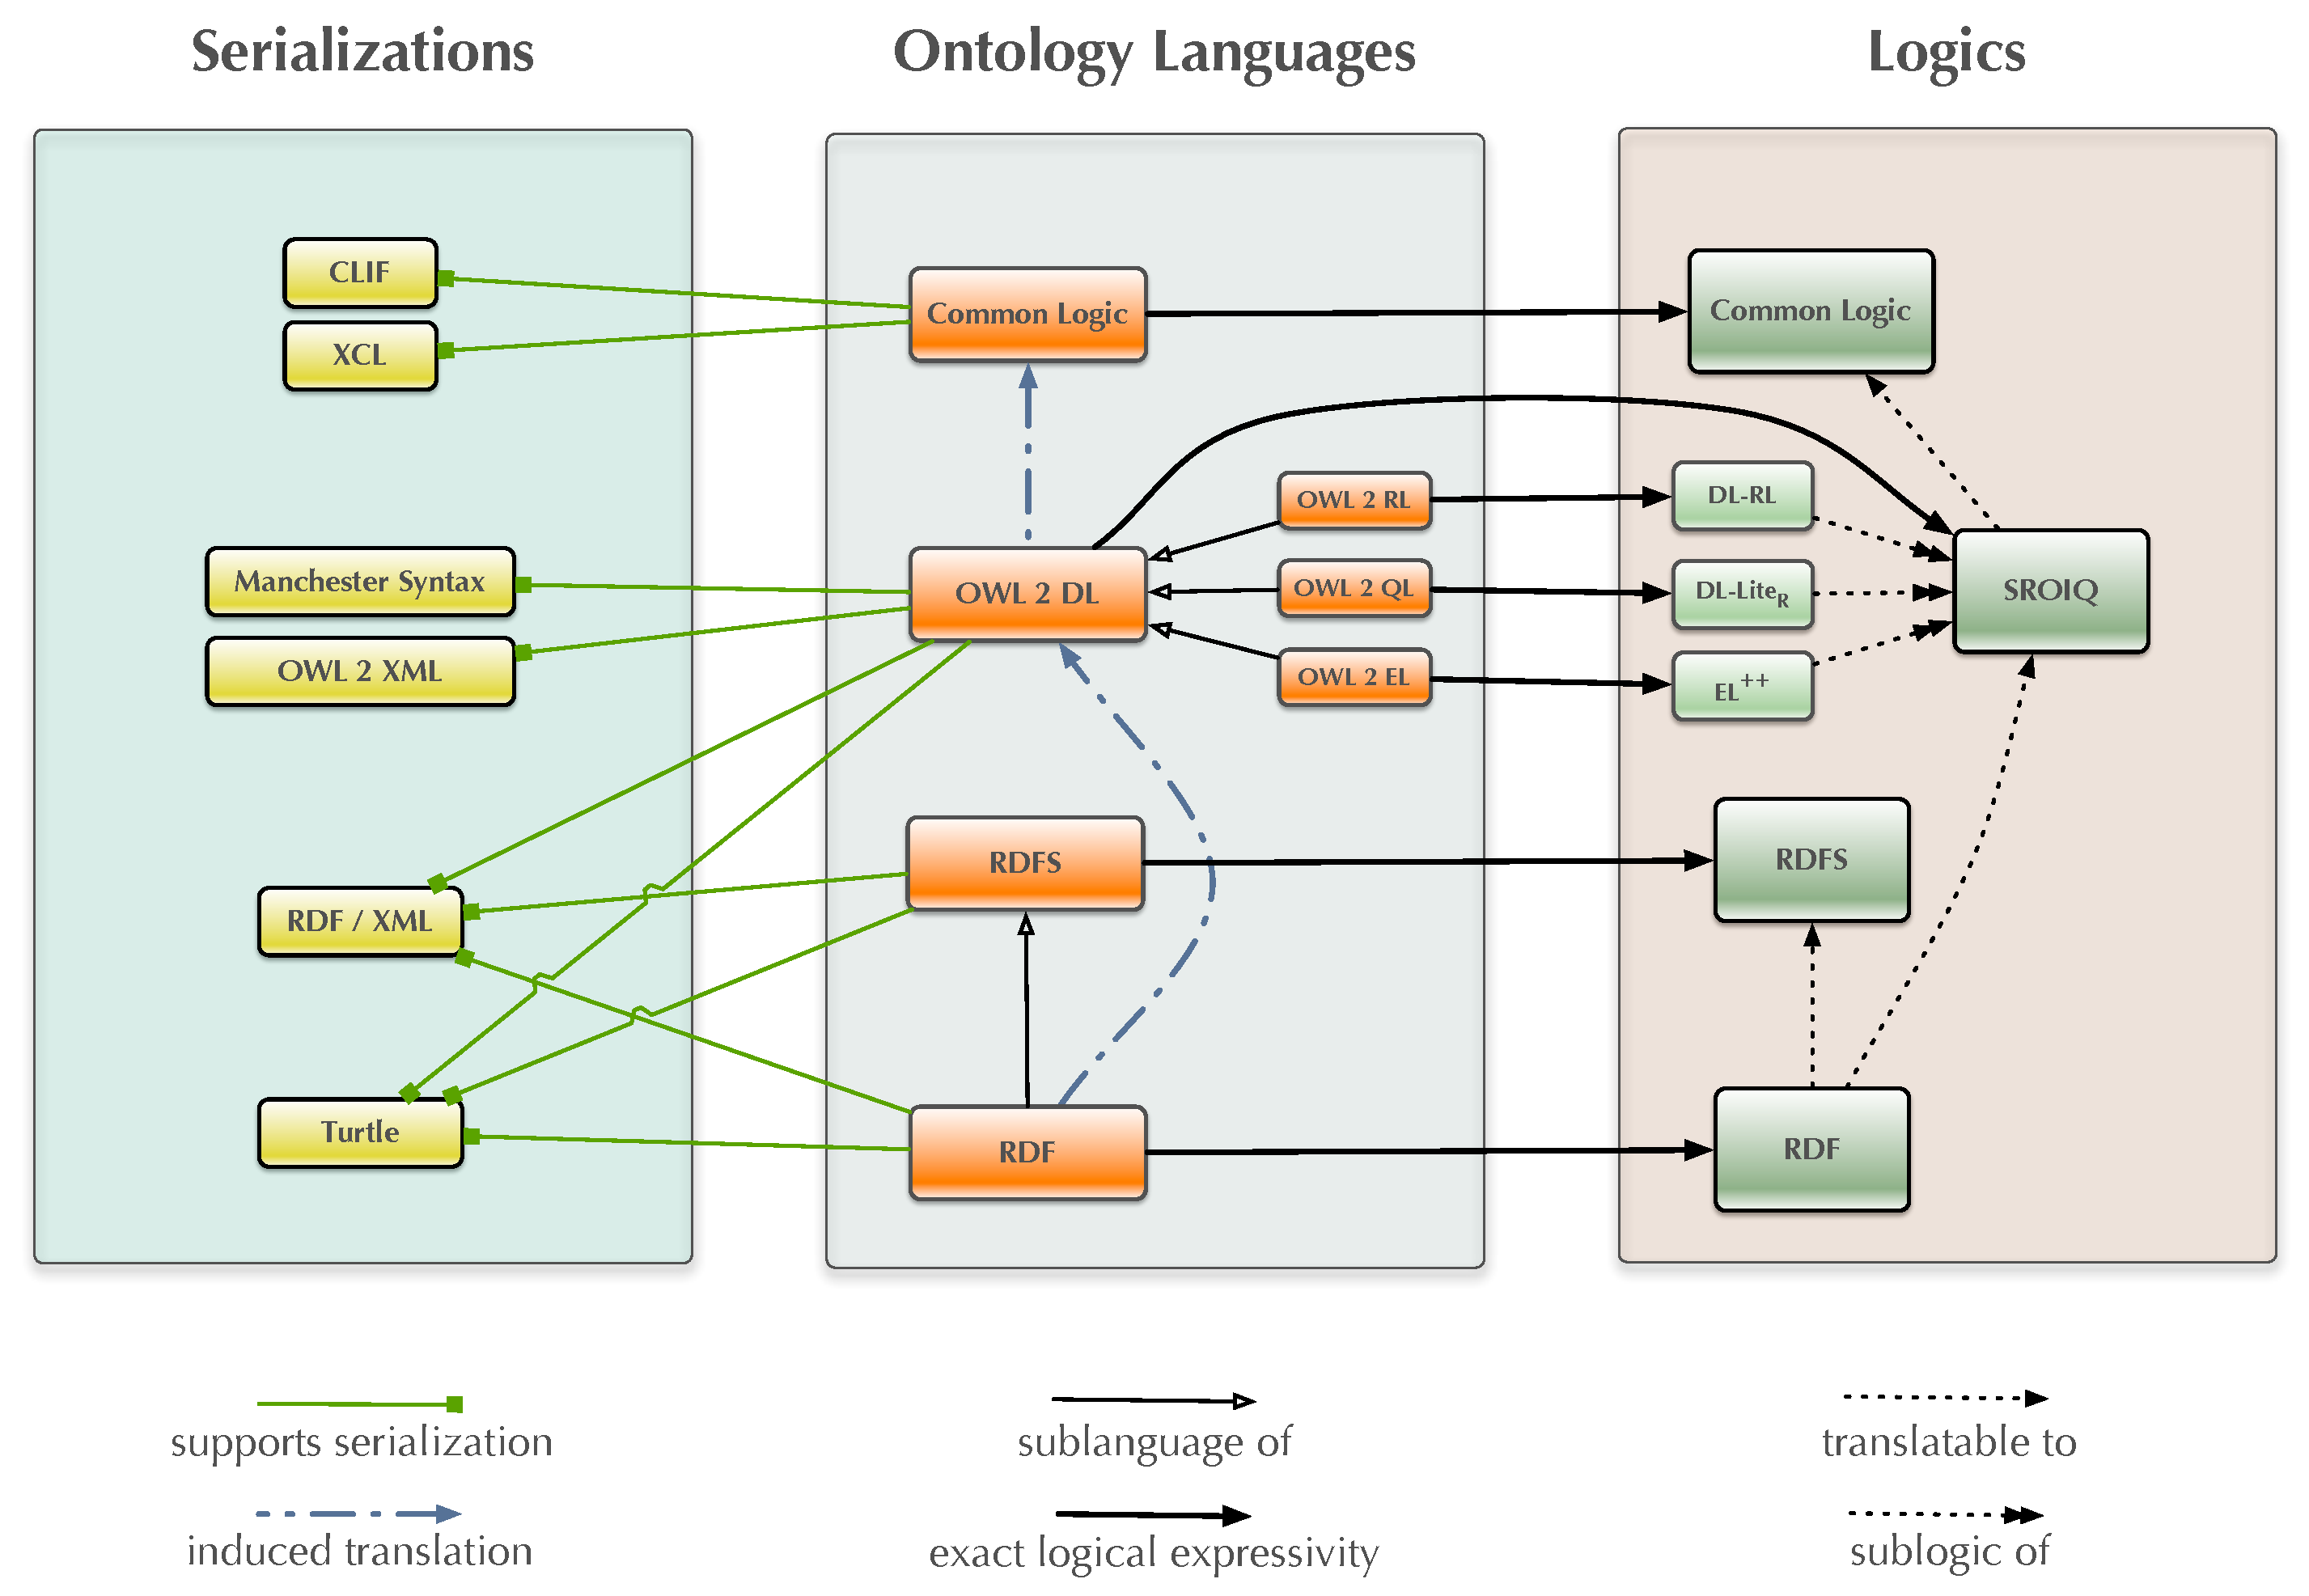
\includegraphics[width=\textwidth]{illustrations/DOL-ontograph-layers-ISO} 
  \caption{Subset of the OntoIOp registry, shown as an RDF graph}
\label{f:DOL-threelayers}
\end{figure}

This annex specifies an RDF vocabulary, formalized in RDFS \nisref{W3C/TR REC-rdf-schema:2004}, for describing OMS languages that conform with DOL, and their features, including logics and serializations.  This vocabulary shares its namespace (\url{http://purl.net/dol/1.0/rdf#}) with the DOL RDF vocabulary for serializing DOL OMS (\cf \aref{a:rdf-syntax}).\CLnote[type=fyi]{given its light weight I think that makes sense.  It doesn't rule out extensions to OWL (or even DOL) anyway.}  

The tables in this annex list the classes and properties of the RDF vocabulary for describing OMS languages.  All class and properties are assumed to be in the DOL RDF namespace unless stated otherwise.

\tref{tab:logic-vocab-classes} lists the classes of the RDF vocabulary for describing OMS languages.  Each row of the table translates into the following RDF triples (given in Turtle serialization):\CLnote[type=todo]{also cover rdfs:subClassOf (once we have such cases)}

\begin{lstlisting}[language=N3]
_:class rdf:type     rdfs:Class ;
        rdfs:comment "documentation" .
\end{lstlisting}

\newcommand*{\ClassDocumentation}[1]{\textit{#1}}
\ctable[
caption={Classes of the RDF vocabulary for describing OMS languages},
mincapwidth=\textwidth,
label={tab:logic-vocab-classes},
pos=h,
]{ll}{% table footnotes
}{\FL
  Class & \ClassDocumentation{documentation}\ML
  OMSLanguage & \ClassDocumentation{an OMS language}\NN
  Logic & \ClassDocumentation{a logic that defines the semantics of an OMS language}\NN
  Serialization & \ClassDocumentation{a serialization of an OMS language}\LL
}

\tref{tab:logic-vocab-prop} lists the properties of the RDF vocabulary for describing OMS languages.  Each row of the table translates into the following RDF triples (given in Turtle serialization):

\begin{lstlisting}[language=N3]
_:property rdf:type     rdf:Property ;
           rdfs:domain  _:domain ;
           rdfs:range   _:range ;
           rdfs:comment "documentation" .
\end{lstlisting}

\todonote[type=q-aut,author=Christoph Lange]{we need to define ``sublogic'' as a term – how?  I guess that would include the notion of an ``OWL profile''}
\newcommand*{\PropertyDocumentation}[1]{\NN\multicolumn{3}{p{\linewidth}}{\textit{#1}}}
\ctable[
caption={Properties of the RDF vocabulary for describing OMS languages},
width=\linewidth,
mincapwidth=\textwidth,
label={tab:logic-vocab-prop},
pos=h,
]{lll}{% table footnotes
}{\FL
  Property & domain & range
  \PropertyDocumentation{documentation}\ML
  subLogicOf & Logic & Logic
  \PropertyDocumentation{The subject is a sublogic of the object}\ML
  supportsLogic & OMSLanguage & Logic
  \PropertyDocumentation{The subject OMS language has a semantics specified in terms of the object logic.}\ML
  specifiesSemanticsOf & Logic & OMSLanguage
  \PropertyDocumentation{The subject logic is used to specify the semantics of the object OMS language; inverse of supportsLogic.}\ML
  supportsSerialization & OMSLanguage & Serialization
  \PropertyDocumentation{OMS in the subject OMS language can be serialized in the object serialization.  Note that the serialization should be as specific as possible, \ie one should not say that ``OWL can be serialized in XML'' and ``Common Logic can be serialized in XML'', but instead ``OWL can be serialized in OWL/XML'' and ``Common Logic can be serialized in XCL'', taking into account that OWL/XML and XCL are two different XML languages.}\ML
  serializes & Serialization & OMSLanguage
  \PropertyDocumentation{The subject logic is used to specify the semantics of the object OMS language; inverse of supportsSerialization.}\LL
}

\normannex{Conformance of OWL 2 with DOL}\label{a:owl}

The semantic conformance of OWL 2 (as specified in \nisref{W3C/TR REC-owl2-syntax:2009}) with DOL is established in \cite{OntoGraph}.

The OWL/XML serialization satisfies the criteria for XML conformance.  The mapping of OWL 2 to RDF graphs satisfies the criteria for RDF conformance\CLnote{This is not exactly true, as some things, e.g. imports, can't be identified.}.  The OWL 2 Manchester syntax satisfies the criteria for text conformance.
~\CLnote{also need conformance propositional logic; use PL ``profile'' of the CASL ``IFIP standard''}

OWL can be formalized as an institute as follows:
\begin{definition}\label{DL} \defsty{\OWL2 DL.} 
\OWL~2~DL is the description logic (DL) based fragment of the web ontology language \OWL 2. 
We start with the simple description logic $\ALC$, and then proceed
to the more complex description logic \SROIQ which is underlying \OWL~2~DL.
Signatures of the description logic $\ALC$ consist of a set  ${\mathcal A}$ of
atomic concepts, a set ${\mathcal R}$ of roles and a set ${\mathcal
I}$ of individual constants. The partial order on signatures is defined
as component wise inclusion.
  Models are 
 first-order structures $I = (\Delta^I, .^I)$ with universe $\Delta^I$
that interpret concepts as unary and roles as binary predicates
(using $.^I$). $I_1\leq I_2$ if $\Delta^{I_1}=\Delta^{I_2}$ and all
concepts and roles of $I_1$ are subconcepts and subroles of those in $I_2$.
Sentences are subsumption relations $C_1\sqsubseteq C_2$ between
concepts, where concepts follow the grammar\CLnote[type=q-aut]{This grammar should also be adapted to ISO EBNF.}
$$C ::= {\mathcal A} \,|\, \top\,|\, \bot \,|\, C_1 \sqcup C_2 \,|\, C_1 \sqcap C_2 \,|\, \neg C 
    \,|\, \forall R . C \,|\, \exists R . C$$
These kind of sentences are also called TBox sentences.
 Sentences can also be ABox sentences, which are
membership assertions of individuals in concepts (written $a:C$ for
$a\in{\mathcal I})$ or pairs of individuals in roles (written $R(a,b)$
for $a,b\in{\mathcal I}, R\in{\mathcal R}$).   Satisfaction is the
standard satisfaction of description logics.

The logic \SROIQ \cite{SROIQ}, which is the logical core of the Web Ontology
Language \OWL 2 DL\footnote{See also \url{http://www.w3.org/TR/owl2-overview/}}, extends $\ALC$ with the following
constructs: (i) complex role inclusions such as $R \circ S \sqsubseteq S$
as well as simple role hierarchies such as $R \sqsubseteq S$,
assertions for symmetric, transitive, reflexive, asymmetric and
disjoint roles (called RBox sentences, denoted by $\mathcal{SR}$), as well as the construct
$\exists R . \mathsf{Self}$ (collecting the set of `$R$-reflexive
points'); (ii) nominals, i.e.\ concepts of the form $\{a\}$, where $a\in\mathcal{I}$ (denoted by $\mathcal{O}$); (iii) inverse
roles (denoted by $\mathcal{I}$); qualified and unqualified number
restrictions ($\mathcal{Q}$). For details on the rather complex
grammatical restrictions for \SROIQ (e.g.\ regular role inclusions,
simple roles) compare \cite{SROIQ}.

\OWL \emph{profiles} are syntactic restrictions of \OWL~2~DL that support specific modeling and reasoning tasks, %\cite{w3c:owl2-profiles}, 
and which are accordingly based on DLs with appropriate computational properties. Specifically, \OWL~2~\EL is designed for ontologies containing large numbers of concepts or relations, \OWL~2~\QL to support query answering over large amounts of data, and \OWL~2~\RL to support scalable reasoning using rule languages (\EL, \QL, and \RL for short) .
 
We sketch the logic \ELDL which is underlying the \EL profile.\footnote{To be exact, \EL adds various `harmless' expressive means and syntactic sugar to \ELDL resulting in the DL \ELDL$++$. % \cite{BaaderEtAl-OWLED08DC}; for further details see also \cite{w3c:owl2-profiles}.
} 
\ELDL is a syntactic restriction of \ALC to existential restriction, concept
intersection, and the top concept:
%\ednote{TM@OK: please be  a bit more precise here, perhaps write some grammar: C ::= ⊤ | A | C ⊓ D | ∃r.C, footnote about added sugar in OWL EL profile} Note that \EL is a very relevant ontology language; large medical ontologies like SNOMED\ednote{CL@TM: FYI, it's SNO not SNOW} CT are epxressed in \EL.\ednote{TM@OK: add RL and QL if there is space}
%\ednote{Text entfernt: ``I.e.\ its concepts follow the following grammar'' -- versteht sich IMHO von selbst, nachdem man das obige \ALC-Beispiel gelesen hat}
$$C ::= {\mathcal A} \,|\, \top \,|\,  C_1 \sqcap C_2 \,|\, \exists R . C$$
Note that \ELDL does not have disjunction or negation, and is therefore a sub-Boolean logic.
\end{definition}


\normannex{Conformance of Common Logic with DOL}\label{a:cl}

The semantic conformance of Common Logic (as specified in \nisref{ISO/IEC 24707:2007}) with DOL is established in \cite{OntoGraph}.

The XCF dialect of Common Logic has a serialization that satisfies the criteria for XML conformance.  The CLIF dialect of Common Logic has a serialization that satisfies the criteria for text conformance.

Common Logic can be defined as an institute as follows:

\begin{definition}\label{CommonLogic} \defsty{Common Logic.}  
A common logic signature
$\Sigma$ (called vocabulary in Common Logic terminology) consists of a
set of names, with a subset called the set of discourse names, and a
set of sequence markers. An inclusion of signatures needs to fulfill the
requirement that a name is a discourse
name in the smaller signature if and only if it is one in the larger signature.  A $\Sigma$-model $I=(\UR,\UD,\rel,\fun,\intCL)$ consists of a set $\UR$,
the universe of reference, with a non-empty subset $\UD\subseteq \UR$,
the universe of discourse, and four mappings:
  \begin{itemize}
   \item $\rel$ from $\UR$ to subsets of $\UD^* = \{<x_1,\ldots,x_n> |
x_1,\ldots,x_n \in \UD\}$ (i.e., the set of finite sequences of
elements of $\UD$);
   \item $\fun$ from $\UR$ to total functions from $\UD^*$ into $\UD$;
   \item $\intCL$ from names in $\Sigma$ to $\UR$, such that
$\intCL(v)$ is in $\UD$ if and only if $v$ is a discourse name;
   \item $\seq$ from sequence markers in $\Sigma$ to $\UD^*$.
  \end{itemize}  A $\Sigma$-sentence is a first-order
sentence, where predications and function applications are written
in a higher-order like syntax: $t(s)$.
Here, $t$ is an arbitrary term, and $s$ is a sequence term, which can
be a sequence of terms $t_1\ldots t_n$, or a sequence marker.
A predication $t(s)$ is interpreted by evaluating the term $t$,
mapping it to a relation using $\rel$, and then asking whether the sequence
given by the interpretation $s$ is in this relation.  
Similarly, a function application $t(s)$ is interpreted using $\fun$.
Otherwise, interpretation of terms and formulae is as in
first-order logic. 
A further
difference is the presence of sequence terms (namely sequence markers and
juxtapositions of terms), which denote sequences in $\UD^*$, with term
juxtaposition interpreted by sequence concatenation.
Note that sequences are essentially a non-first-order feature that
can be expressed in second-order logic.

Model reducts are defined in the following way: 
Given a signature inclusion $\Sigma'\leq\Sigma$ and a $\Sigma$-model
$I=(\UR,\UD,\rel,\fun,\intCL)$, $I\forget{\Sigma'}=(\UR',\UD,\rel',\fun',\intCL')$ is defined by
\begin{itemize}
\item $UR'$ is the restriction of $\UR$ to those elements satisfying the
following conditions:
\begin{enumerate}
\item they are not in the universe of discourse $\UD$;
\item they are the interpretation (according to $\intCL$) of a non-discourse name in $\Sigma$;
\item they are not the interpretation (according to $\intCL$) of a non-discourse name in $\Sigma'$.
\end{enumerate}
\item $\rel'$ is $\rel$ restricted to $\UR'$;
\item $\fun'$ is $\fun$ restricted to $\UR'$;
\item $\intCL'$ is $\intCL$ restricted to $\Sigma'$.
\end{itemize}

Note that with this notion of reduct, extensions commonly understood
as definitions in segregated dialects of Common Logic are indeed both
definitional and conservative extensions.

\todonote{Ordering on models! Universes agree, $\fun_1(x)= \fun_2(x)$, $\rel_1(x)\subseteq \rel_2(x)$, $\intCL_1(n)=\intCL_2(n)$
}

%For details, see \cite{CommonLogic:oldfashioned}.
We call the restriction of \CL to sentence
without sequence markers \CLminus.
\end{definition}


\normannex{Conformance of RDF and RDFS with DOL}\label{a:rdfs}

The semantic conformance of RDFS (as specified in \nisref{W3C/TR REC-rdf-schema:2004}) with DOL is established in \cite{OntoGraph}.

The way of representing RDFS ontologies as RDF graphs satisfies the criteria for RDF conformance.


\begin{definition}[\RDF and \RDFS]
Following \cite{Lucanu}, 
we define the institutions for the Resource Description
Framework (\RDF) and \RDF-Schema (\RDFS), respectively. 
These are based on a logic called \emph{bare} \RDF (\SimpleRDF), which consists
of triples only (without any predefined resources).

%%%%%%%%%%
A \textit{signature} $\mathbf{R_s}$ in \SimpleRDF is a set of
\textit{resource references}. For $sub, pred, obj \in \mathbf{R_s}$, a
triple of the form $(sub, pred, obj)$ is a \textit{sentence} in \SimpleRDF,
where $sub$, $pred$, $obj$ represent subject name, predicate name,
object name, respectively. An $\mathbf{R_s}$-model $M =
\langle R_m, P_m, S_m, EXT_m \rangle$ consists of a \textit{set $R_m$
  of resources}, a set $P_m \subseteq R_m$ of predicates, a
\textit{mapping function} $S_m:\mathbf{R_s} \rightarrow R_m$, and an
\textit{extension function} $EXT_m: P_m \rightarrow \mathcal{P}(R_m
\times R_m)$ mapping every predicate to a set of pairs of
resources. Satisfaction is defined as follows:
%
\[\mathfrak{M} \models_{\mathbf{R_s}} (sub, pred, obj) \Leftrightarrow (S_{m}(sub),
(S_{m}(obj)) \in EXT_{m} (S_m(pred)). \]
%%%%%
%
Both \RDF and \RDFS are built on top of \SimpleRDF by fixing a certain
standard vocabulary both as part of each signature and in the models.\ednote{Refer to the RDF standard here.}
Actually, the standard vocabulary is given by a certain theory. In case
of \RDF, it contains e.g.\ resources \texttt{rdf:type} and
\texttt{rdf:Property} and \texttt{rdf:subject}, and sentences like, e.g.\
$(\texttt{rdf:type},\texttt{rdf:type},$ $ \texttt{rdf:Property})$, and $(\texttt{rdf:subject}, \texttt{rdf:type},$  $\texttt{rdf:Property})$.

In the models, the standard vocabulary is interpreted with a fixed
model.  Moreover, for each $\RDF$-model $M = \langle R_m, P_m, S_m,
EXT_m \rangle$, if $p\in P_m$, then it must hold
$(p,S_m(\texttt{rdf:Property}))\in EXT_m(\texttt{rdf:type})$.
For \RDFS, similar conditions are formulated (here, for example also
the subclass relation is fixed).


In the case of \RDFS, the standard vocabulary contains more elements,
like
rdf:domain,
rdf:range, rdf:Resource, rdf:Literal, rdf:Datatype, rdf:Class,
rdf:subClassOf, rdf:subPropertyOf, rdf:member, rdf:Container,
rdf:ContainerMembershipProperty.

There is also \OWL full, an extension of \RDFS with resources
like owl:Thing and owl:oneOf, tailored towards the representation of
\OWL.

\end{definition}


\normannex{A Core Logic Graph}\label{a:graph}

\begin{figure}
  \centering
  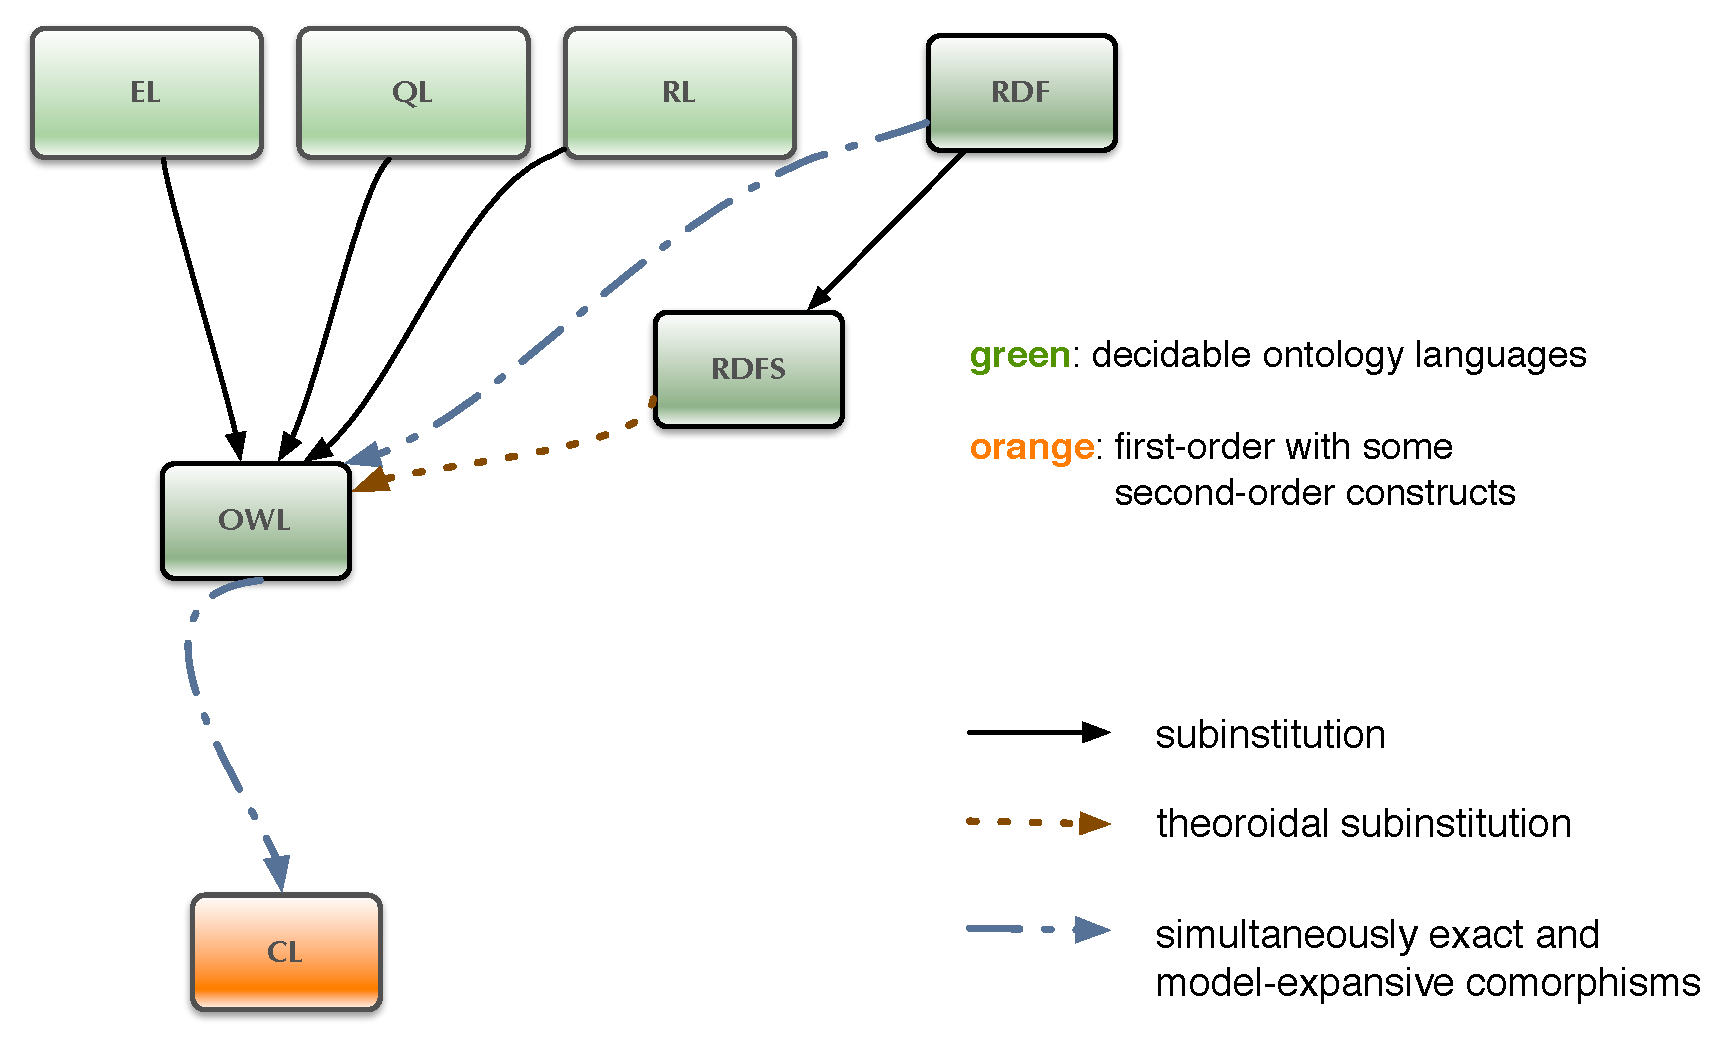
\includegraphics[width=\textwidth]{illustrations/ontograph-standards}
  \caption{Translations between conforming OMS languages (normative)}
  \label{fig:ontograph-standards}
\end{figure}
This annex provides a core graph of logics and translations, covering those OMS languages whose conformance with DOL is established in the preceding, normative annexes (OWL 2 in \aref{a:owl}, Common Logic in \aref{a:cl}, and RDFS in \aref{a:rdfs}).  The graph is shown in \fref{fig:ontograph-standards}.  Its nodes refer to the following OMS languages and profiles:
\begin{itemize}
\item RDF \nisref{W3C/TR REC-rdf-concepts:2004}
\item RDFS \nisref{W3C/TR REC-rdf-schema:2004}
\item EL, QL, RL (all being profiles of OWL) \nisref{W3C/TR REC-owl2-profiles:2009}
\item OWL \nisref{W3C/TR REC-owl2-syntax:2009}
\item CL (Common Logic) \nisref{ISO/IEC 24707:2007}
\end{itemize}
The translations are specified in \cite{OntoGraph}.
~\todonote[author=Christoph Lange,type=todo]{Provide linear syntax here (as in the paper)}

~\todonote[author=Christoph Lange,type=fyi]{We need this in order to be able to say something about default translations, and about establishing conformance by translation to a language that already conforms.}



\sclause{\EL $\to$ $\OWL$ and $\ELDL++$ $\to$ $\SROIQ(D)$}

\EL $\to$ $\OWL$ is the sublanguage inclusion obtained by the
syntactic restriction according to the definition of \EL, see
\nisref{W3C/TR REC-owl2-profiles:2009}. Since by definition, $\ELDL++$
is a syntactic restriction of $\SROIQ(D)$, $\ELDL++$ $\to$ $\SROIQ(D)$
is the corresponding sublogic inclusion.

\sclause{\QL $\to$ $\OWL$ and \DLLiteR $\to$ $\SROIQ(D)$}

\QL $\to$ $\OWL$ is the sublanguage inclusion obtained by the
syntactic restriction according to the definition of \QL, see
\nisref{W3C/TR REC-owl2-profiles:2009}. Since by definition, \DLLiteR
is a syntactic restriction of $\SROIQ(D)$, \DLLiteR $\to$ $\SROIQ(D)$
is the corresponding sublogic inclusion.

\sclause{\RL $\to$ $\OWL$ and $\RL$ $\to$ $\SROIQ(D)$}

\RL $\to$ $\OWL$ is the sublanguage inclusion obtained by the
syntactic restriction according to the definition of \RL, see
\nisref{W3C/TR REC-owl2-profiles:2009}. Since by definition, $\RL$
is a syntactic restriction of $\SROIQ(D)$, $\RL$ $\to$ $\SROIQ(D)$
is the corresponding sublogic inclusion.

\sclause{$\SimpleRDF \rightarrow \RDF$}

$\SimpleRDF \rightarrow \RDF$ is an obvious inclusion, except that
\SimpleRDF resources need to be renamed if they happen to have a predefined
meaning in \RDF. The model translation needs to forget the fixed parts
of \RDF models, since this part can always reconstructed in a unique
way, we get an isomorphic model translation. 

\sclause{$\RDF \rightarrow \RDFS$}

This is entirely analogous to $\SimpleRDF \rightarrow \RDF$.

\sclause{$\SimpleRDF \rightarrow \SROIQ(D)$}

\todonote{This translation is not really useful. Consider the
  RDF-OWL-reduct construction instead.}


A $\SimpleRDF$ signature is translated to $\SROIQ(D)$ by providing a class
$P$ and three roles $sub$, $pred$ and $obj$ (these reify the extension
relation), and one individual per $\SimpleRDF$ resource. A $\SimpleRDF$ triple
$(s,p,o)$ is translated to the \SROIQ(D) sentence
   $$\top \sqsubseteq \exists U. (\exists sub. \{s\} \sqcap \exists pred. \{p\} \sqcap  \exists obj. \{o\} ).$$
  From an \SROIQ(D) model ${\cal I}$, obtain a \SimpleRDF model by inheriting the universe
  and the interpretation of individuals (then turned into resources).
  The interpretation $P^{\cal I}$ of $P$ gives $P_m$, and $EXT_m$ is obtained
  by de-reifying,
 i.e. $$EXT_{m}(x):=\{(y,z) | \exists u . (u,x)\in pred^{\cal I},
  (u,y)\in sub^{\cal I}, (u,z,)\in obj^{\cal I} \}.$$
  $\RDF \rightarrow \SROIQ(D)$ is defined similarly. The theory of \RDF built-ins 
  is (after translation to \SROIQ(D)) added to any signature translation.
  This ensures that the model translation can add the built-ins.
%\Til{What if the OWL model satisfies more triples than the built-ins?}

\sclause{$\OWL \rightarrow FOL$}

\ssclause{Translation of Signatures}

 $\Phi((\Concepts, \Roles, \Individuals)) =  (F, P)$ with
\begin{itemize}
	\item function symbols: $F = \{a^{(1)} \vert a \in \Individuals\}$
	\item predicate symbols $P = \{A^{(1)} \vert A \in \category{C} \} \cup \{ R^{(2)} \vert R \in \category{R}\}$
\end{itemize}


\ssclause{Translation of Sentences}

Concepts are translated as follows:
\begin{itemize}
 \item $\alpha_x(A) = A(x)$
 \item $\alpha_x(\lnot C) = \lnot \alpha_x (C)$
 \item $\alpha_x(C \sqcap D) = \alpha_x(C) \land \alpha_x(D)$
 \item $\alpha_x(C \sqcup D) = \alpha_x(C) \lor \alpha_x(D)$ 
 \item $\alpha_x(\exists R.C) = \exists y . (R(x,y) \land \alpha_y(C))$
 \item $\alpha_x(\exists U.C) = \exists y . \alpha_y(C)$
 \item $\alpha_x(\forall R.C) = \forall y . (R(x,y) \rightarrow \alpha_y(C))$
 \item $\alpha_x(\forall U.C) = \forall y . \alpha_y(C)$
 \item $\alpha_x(\exists R.\text{Self}) = R(x,x)$
 \item $\alpha_x(\leq n R. C) = \forall y_1,\ldots,y_{n+1} .  \bigwedge_{i=1,\ldots,n+1}(R(x,y_i) \land \alpha_{y_i}(C)) \rightarrow\bigvee_{1\leq i<j\leq n+1}y_i = y_j$
 \item $\alpha_x(\geq n R. C) = \exists y_1,\ldots,y_n . \bigwedge_{i=1,\ldots,n}(R(x,y_i) \land \alpha_{y_i}(C)) \wedge \bigwedge_{1\leq i<j\leq n}y_i\not= y_j $
 \item $\alpha_x(\{a_1, \ldots a_n \}) = (x=a_1\vee \ldots \vee x=a_n)$
\end{itemize}

For inverse roles $R^-$, $R^-(x,y)$ has to be replaced by $R(y,x)$, e.g.
 $$\alpha_x(\exists R^-.C) = \exists y . (R(y,x) \land \alpha_y(C))$$
This rule also applies below.


Sentences are translated as follows:

\begin{itemize}
 \item $\alpha_\Sigma (C \sqsubseteq D) = \forall x.\, (\alpha_x(C) \rightarrow \alpha_x(D))$
 \item $\alpha_\Sigma (a:C) = \alpha_x(C)[a/x]$\footnote{Replace $x$ by $a$.}
 \item $\alpha_\Sigma (R(a,b)) = R(a,b)$
 \item $\alpha_\Sigma (R \sqsubseteq S) = \forall x, y. R(x,y) \rightarrow S(x,y) $
 \item $\alpha_\Sigma (R_1; \ldots; R_n \sqsubseteq R) =$\\
$ \forall x,y . (\exists z_1,\ldots z_{n-1} . R_1(x,z_1) \wedge R_2(z_1,z_2) \wedge \ldots \wedge R_n(z_{n-1},y)) \rightarrow R(x,y) $
 \item $\alpha_\Sigma (\text{Dis}(R_1,R_2)) = \neg\exists x,y . R_1(x,y)\wedge R_2(x,y)$	
 \item $\alpha_\Sigma (\text{Ref}(R)) = \forall x. R(x,x)$
 \item $\alpha_\Sigma (\text{Irr}(R)) = \forall x. \neg R(x,x)$
 \item $\alpha_\Sigma (\text{Asy}(R)) = \forall x,y . R(x,y) \rightarrow \neg R(y,x)$
 \item $\alpha_\Sigma (\text{Tra}(R)) = \forall x,y,z . R(x,y) \wedge R(y,z) \rightarrow R(x,z)$
\end{itemize}





\ssclause{Translation of Models}

\begin{itemize}
	\item For $M' \in \Models^{FOL}(\Phi \Sigma)$ define $\beta_\Sigma(M') := (\Delta, \cdot^I)$
	with $\Delta = |M'|$ and $A^I = M'_A, a^I = M'_a, R^I = M'_R$.
\end{itemize}

	\begin{proposition}
$C^\I = \left\{m \in M'_{\Thing} \lvert M' + \{x \mapsto m \} \models \alpha_x (C) \right\}$
	\end{proposition}
	
	\begin{proof} By Induction over the structure of $C$.
\begin{itemize}
	\item $A^\I = M'_A = \left \{m \in M'_{\Thing} \vert M' + \{x \mapsto m \} \models A(x)  \right\}$
	\item $(\lnot C)^\I = \Delta \setminus C^\I =^{I.H.} \Delta \setminus \{m \in M'_\Thing \lvert M' + \{x \mapsto m\} \models \alpha_x(C)\} = \{m \in M'_\Thing \vert M' + \{x \mapsto m\} \models \lnot \alpha_x(C)\}$
\end{itemize}
	\end{proof}

	The satisfaction condition holds as well.

\sclause{$\OWL \rightarrow \CL$}


\infannex{Extended Logic Graph}\label{a:ext-graph}

\begin{figure}
  \centering
  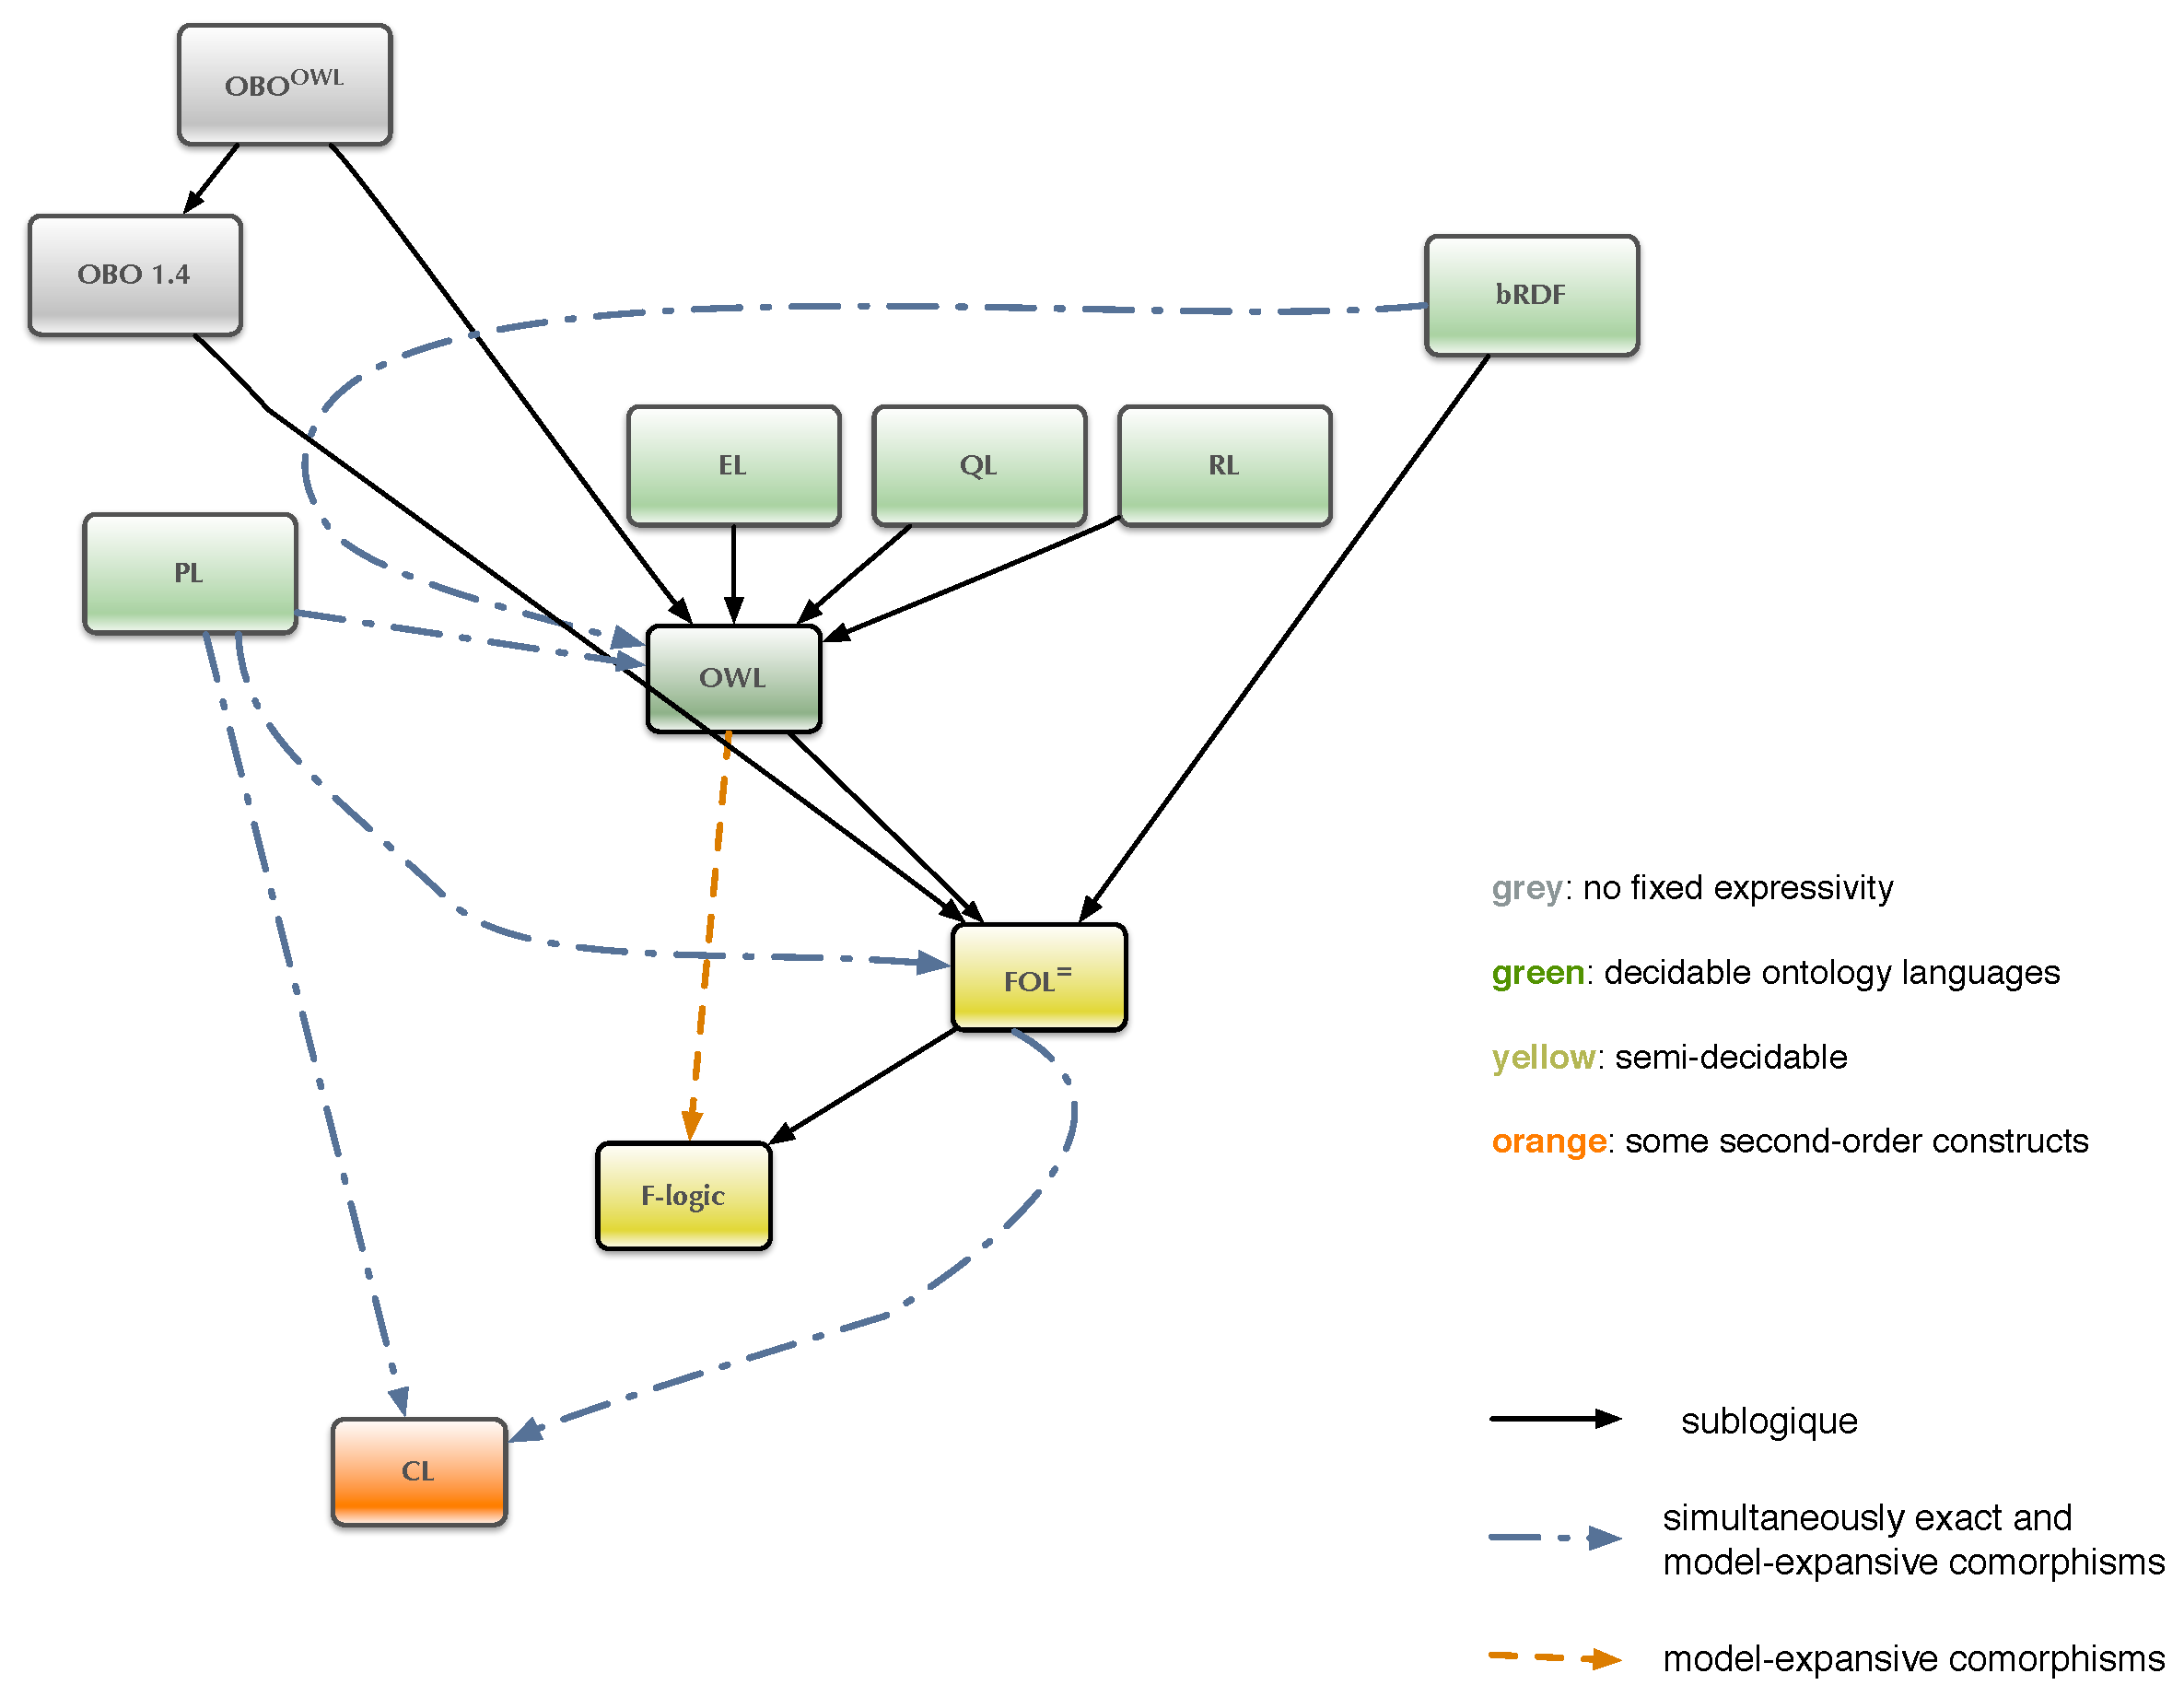
\includegraphics[width=\textwidth]{illustrations/pre-reduced-ontograph}
  \caption{Translations between conforming OMS languages (extended)}
  \label{fig:pre-ontograph}
\end{figure}
This annex extends the graph of logics and translations given in
\aref{a:graph} by a list of OMS language whose conformance with
DOL will be established through the registry.  The graph is shown in
\fref{fig:pre-ontograph}.  Its nodes are included in the following
list of OMS languages and profiles (in addition to those
mentioned in \aref{a:graph}):
\begin{itemize}
\item PL (propositional logic)
\item SimpleRDF (RDF triples without a reserved vocabulary)
\item OBO\textsuperscript{OWL} and OBO1.4
\item RIF (Rule Interchange Format)
\item EER (Enhanced Entity-Relationship Diagrams) % see Talheim Thalheim, B. (2009). Extended entity relationship model. In L. Liu and M. T. Ozsu, editors, En- cyclopedia of Database Systems, volume 1, pages 1083-1091. Springer.
\item Datalog
\item ORM (object role modeling)
\item the meta model of schema.org
\item UML (Unified Modeling Language), with possibly different logics according to different
UML semantics
\item SKOS (Simple Knowledge Organization System )
\item FOL\textsuperscript{=} (untyped first-order logic, as used for the
TPTP format)
\item F-logic
\item CASL (Common Algebraic Specification Language)
\end{itemize}

The actual translations are specified in \cite{OntoGraph}.

~\todonote[author=Christoph Lange,type=todo]{Provide linear syntax here (as in the paper). TM: what do you mean by this?}



\infannex{Example Uses of all DOL Constructs}

\ednote{the uses cases in the RFP should be reused and worked into DOL examples}

\CLnote[type=q-aut]{Should we have another column here that refers to the \emph{abstract} syntax?}%
\begin{tabular}{|l|l|}\hline
\multicolumn{2}{|c|}{\textbf{Top-level declarations in libraries}}\\\hline
\textbf{Top-level declaration} & \textbf{Examples} \\\hline
language IRI  & Alignments, Publications \\\hline
logic IRI  & Alignments, Mereology \\\hline
serialization IRI  & Alignments, Mereology \\\hline
PrefixMap  & Mereology \\\hline
ontology IRI = OMS end  &  Alignments, Mereology \\\hline
ontology IRI = \%mcons OMS end  & Mereology \\\hline
interpretation IRI : OMS to OMS = Symbol |-> Symbol ...  & Mereology \\\hline
interpretation IRI : OMS to OMS = \%cons Symbol |-> Symbol ...  &  \\\hline
interpretation IRI : OMS to OMS = translation IRI  & Mereology \\\hline
equivalence IRI : OMS \lessthan-\greaterthan\ OMS = OMS end  &  Algebra \\\hline
module IRI : OMS of OMS for Symbols  &  \\\hline
module IRI \%ccons : OMS of OMS for Symbols  &  \\\hline
alignment IRI : OMS to OMS end  &  \\\hline
alignment IRI 1 : OMS to OMS end  &  \\\hline
alignment IRI ? : OMS to OMS end  &  \\\hline
alignment IRI + : OMS to OMS end  &  \\\hline
alignment IRI * : OMS to OMS end  &  \\\hline
alignment IRI : OMS to OMS = Correspondences  & Alignments \\\hline
\end{tabular}

\begin{tabular}{|l|l|}\hline
\multicolumn{2}{|c|}{\textbf{OMS}}\\\hline
\textbf{OMS notation} & \textbf{Examples} \\\hline
BasicOMS  & Alignments, Mereology \\\hline
IRI  & Alignments, Mereology \\\hline
IRI \%( IRI )\%  &  \\\hline
minimize \{ OMS \}  & BlocksWithCircumscription \\\hline
OMS minimize Symbols var Symbols  & BlocksWithCircumscription \\\hline
OMS with Symbol |-> Symbol ...  & Alignments \\\hline
OMS with translation IRI  & Mereology \\\hline
OMS with translation IRI : IRI $\to$ IRI  &  \\\hline
OMS with translation IRI $\to$ IRI  &  \\\hline
OMS with translation $\to$ IRI  &  \\\hline
OMS hide SymbolItems  &  Algebra \\\hline
OMS reveal Symbols  &  \\\hline
OMS reveal Symbol |-> Symbol ...  &  \\\hline
OMS hide along IRI  &  \\\hline
OMS hide along IRI : IRI $\to$ IRI  &  \\\hline
OMS hide along IRI $\to$ IRI  &  \\\hline
OMS hide along $\to$ IRI  &  \\\hline
OMS approximate with IRI   &  \\\hline
OMS approximate in IRI with IRI   &  \\\hline
OMS approximate in IRI  &  \\\hline
OMS and OMS   &  \\\hline
OMS then OMS  & Mereology \\\hline
OMS then \%ccons OMS  &  \\\hline
OMS then \%ccons \%( IRI )\% OMS  &  \\\hline
OMS then \%mcons OMS  &  \\\hline
OMS then \%mono OMS  &  \\\hline
OMS then \%wdef OMS  &  \\\hline
OMS then \%def OMS  &  \\\hline
OMS then \%implied OMS  &  BlocksWithCircumscription \\\hline
logic IRI : OMS  &  \\\hline
language IRI : OMS  &  \\\hline
serialization IRI : OMS  &  \\\hline
OMS bridge Translation OMS  & Publications \\\hline
combine NetworkElements  & Alignments, Publications \\\hline
combine NetworkElements excluding IRIs  &  \\\hline
\end{tabular}

\sclause{Mereology: Distributed and Heterogeneous Ontologies}
\label{dist-het-onto}
\CLnote[type=q-aut]{In the TKE paper we made the name of the propositional logic ontology syntax explicit.  The propositional logic listing now leaves us with a problem: neither is propositional logic specified as DOL-conformant, nor is Hets' CASL-like syntax, nor is anything of this intended to ever be normative. TM: hence either leave it out, or make propositional logic normative. What about the examples in OWL+CL develop during the Ontology Summit Hackathon?}
\begin{lstlisting}[basicstyle=\ttfamily,language=dolText,morekeywords={props,ObjectProperty,Class,DisjointUnionOf,SubClassOf,Characteristics,Transitive,Asymmetric,SubPropertyOf,DisjointClasses,EquivalentTo,inverse,only,forall,iff,if,or,exists},escapechar=@,mathescape]
%prefix( :      <http://www.example.org/mereology#>
         owl:   <http://www.w3.org/2002/07/owl#>
         log:   <http://purl.net/dol/@logic@/>    %% descriptions of logics ...
         trans: <http://purl.net/dol/translations/> )%  %% ... and translations

library Mereology

logic log:Propositional syntax ser:Prop/Hets       %% non-standard serialization built into Hets 
ontology Taxonomy = %mcons      %% basic taxonomic information about mereology reused from DOLCE
  props PT, T, S, AR, PD
  . S $\vee$ T $\vee$ AR $\vee$ PD $\longrightarrow$ PT                                                    %% PT is the top concept
  . S $\wedge$  T  $\longrightarrow$ $\bot$                                               %% PD, S, T, AR are pairwise disjoint
  . T $\wedge$ AR $\longrightarrow$ $\bot$                                                                         %% and so on
end

language lang:OWL2 logic log:SROIQ syntax ser:OWL2/Manchester           %% OWL Manchester syntax
ontology BasicParthood =                             %% Parthood in SROIQ, as far as easily expressible
  Class: ParticularCategory SubClassOf: Particular
                                            %% omitted similar declarations of the other classes
    DisjointUnionOf: SpaceRegion, TimeInterval, AbstractRegion, Perdurant
                                 %% pairwise disjointness more compact thanks to an OWL built-in
  ObjectProperty: isPartOf        Characteristics: Transitive
  ObjectProperty: isProperPartOf  Characteristics: Asymmetric  SubPropertyOf: isPartOf 
  Class: Atom EquivalentTo: inverse isProperPartOf only owl:Nothing
end                                          %% an atom has no proper parts

interpretation TaxonomyToParthood : Taxonomy to BasicParthood =
  translation trans:PropositionalToSROIQ,    %% translate the logic, then rename the entities
  PT $\mapsto$ Particular, S $\mapsto$ SpaceRegion, T $\mapsto$ TimeInterval, A $\mapsto$ AbstractRegion, %[ and so on ]%

logic log:CommonLogic syntax ser:CommonLogic/CLIF
                      %% syntax: the Lisp-like CLIF dialect of Common Logic
ontology ClassicalExtensionalParthood =
  BasicParthood with translation trans:SROIQtoCL
      %% import the OWL ontology from above, translate it to Common Logic, then extend it there:
then
  . (forall (X) (if (or (= X S) (= X T) (= X AR) (= X PD))
                    (forall (x y z) (if (and (X x) (X y) (X z))
                                        (and                          %% now list all the axioms
      (if (and (isPartOf x y) (isPartOf y x)) (= x y))                           %% antisymmetry
      (if (and (isProperPartOf x y) (isProperPartOf y z)) (isProperPartOf x z))
                              %% transitivity; can't be expressed in OWL together with asymmetry
      (iff (overlaps x y) (exists (pt) (and (isPartOf pt x) (isPartOf pt y))))
      (iff (isAtomicPartOf x y) (and (isPartOf x y) (Atom x)))
      (iff (sum z x y)
           (forall (w) (iff (overlaps w z) (and (overlaps w x) (overlaps w y)))))
      (exists (s) (sum s x y))                                           %% existence of the sum
      )))))
  . (forall (Set a) (iff (fusion Set a)                                  %% definition of fusion
            (forall (b) (iff (overlaps b a)
                             (exists (c) (and (Set c) (overlaps c a)))))))
  }
\end{lstlisting}


\sclause{Blocks World: Minimization}
\CLnote[type=q-aut]{Here we need the prefixes for registry entries (e.g.\ logics) once more; they should be reused across examples.  Or we need to specify a mechanism that gets rid of \emph{these} prefixes altogether.  @TM, could you please comment on my specification enhancement request \texttt{http://trac.informatik.uni-bremen.de:8080/hets/ticket/1020\#comment:33}?}
  \begin{lstlisting}[language=dolText,morekeywords={forall,if,not,Class,Individual,Types,EquivalentTo,SubClassOf,and}]
library BlocksWithCircumscription
logic log:OWL

ontology Blocks = 
  %% FIXED PART 
  Class: Block
  Individual: B1 Types: Block
  Individual: B2 Types: Block DifferentFrom: B1
              %% B1 and B2 are different blocks
then
  %% CIRCUMSCRIBED PART
  minimize {
    Class: Abnormal
    Individual: B1 Types: Abnormal
       %% B1 is abnormal
  }
then
  %% VARYING PART
  Class: Ontable 
  Class: BlockNotAbnormal EquivalentTo: Block and not Abnormal SubClassOf: Ontable 
        %% Normally, a block is on the table
then %implied
  Individual: B2 Types: Ontable
     %% B2 is on the table
end
  \end{lstlisting}

\todo{Instead of Blocks World, perhaps we could specify an ontology that uses inheritance networks with exceptions, and then use circumscription to axiomatize that ontology.}
 
  \begin{lstlisting}[language=dolText,morekeywords={forall,if,not,circ,var,Class,Individual,EquivalentTo,and,SubClassOf}]
ontology Blocks_Alternative =
  Class: Block
  Class: Abnormal
  Individual: B1 Types: Block, Abnormal
  Individual: B2 Types: Block DifferentFrom: B1
              %% B1 and B2 are different blocks
              %% B1 is abnormal
  Class: Ontable 
  Class: BlockNotAbnormal EquivalentTo: Block and not Abnormal SubClassOf: Ontable 
        %% Normally, a block is on the table
  minimize Abnormal var Ontable, BlockNotAbnormal
then %implied
  Individual: B2 Types: Ontable
     %% B2 is on the table
end
  \end{lstlisting}

\ssclause{Alignments}

\begin{lstlisting}[basicstyle=\ttfamily,language=dolText,morekeywords={props,ObjectProperty,Class,DisjointUnionOf,SubClassOf,Characteristics,Transitive,Asymmetric,SubPropertyOf,DisjointClasses,EquivalentTo,inverse,only,forall,iff,if,or,exists,bridge,distributed},escapechar=@,mathescape]
%prefix( :     <http://www.example.org/alignment#>
         owl   <http://www.w3.org/2002/07/owl#>
         log   <http://purl.net/dol/@logic@/> %% descriptions of logics ...
         trans <http://purl.net/dol/translations/> )% %% ... and translations

library Alignments

language lang:OWL2 logic log:SROIQ syntax ser:OWL2/Manchester

alignment Alignment1 : { Class: Woman } to { Class: Person } =
  Woman < Person
end

ontology AlignedOntology1 =
  combine Alignment1
end


ontology Onto1 =
  Class: Person
  Class: Woman SubClassOf: Person
  Class: Bank
end

ontology Onto2 =
  Class: HumanBeing
  Class: Woman SubClassOf: HumanBeing
  Class: Bank
end

alignment VAlignment : Onto1 to Onto2 =
  Person = HumanBeing,
  Woman = Woman
end

ontology VAlignedOntology =
  combine 1 : Onto1, 2 : Onto2, VAlignment
  %% 1:Person is identified with 2:HumanBeing
  %% 1:Woman is identified with 2:Woman
  %% 1:Bank and 2:Bank are kept distinct
end

ontology VAlignedOntologyRenamed =
  VAlignedOntology with 1:Bank |-> RiverBank, 2:Bank |-> FinancialBank
end

\end{lstlisting}


\sclause{Distributed Description Logics}

\begin{lstlisting}[basicstyle=\ttfamily,language=dolText,morekeywords={props,ObjectProperty,Class,DisjointUnionOf,SubClassOf,Characteristics,Transitive,Asymmetric,SubPropertyOf,DisjointClasses,EquivalentTo,inverse,only,forall,iff,if,or,exists,bridge,distributed},escapechar=@,mathescape]
%prefix( :     <http://www.example.org/mereology#>
         owl   <http://www.w3.org/2002/07/owl#>
         log   <http://purl.net/dol/@logic@/> %% descriptions of logics ...
         trans <http://purl.net/dol/translations/> )% %% ... and translations

library Publications

language lang:OWL2 logic log:SROIQ syntax ser:OWL2/Manchester

ontology Publications1 =
  Class: Publication
  Class: Article SubClassOf: Publication
  Class: InBook SubClassOf: Publication
  Class: Thesis  SubClassOf: Publication
  Class: MasterThesis  SubClassOf: Thesis
  Class: PhDThesis SubClassOf: Thesis
end

ontology Publications2 =
  Class: Thing
  Class: Article SubClassOf: Thing
  Class: BookArticle SubClassOf: Thing
  Class: Publication SubClassOf: Thing
  Class: Thesis  SubClassOf: Thing
end

ontology Publications_Combined =
combine
  1 : Publications1 with translation OWL2MS-OWL,
  2 : Publications2 with translation OWL2MS-OWL
  %% implicitly: Article $\mapsto$ 1:Article @\ldots@
  %%             Article $\mapsto$ 2:Article @\ldots@  
bridge with translation MS-OWL2DDL
  %% implicitly added my translation MS-OWL2DDL: binary relation providing the bridge
  1:Publication $\stackrel{\sqsubseteq}{\longrightarrow}$ 2:Publication
  1:PhdThesis $\stackrel{\sqsubseteq}{\longrightarrow}$ 2:Thesis
  1:InBook $\stackrel{\sqsubseteq}{\longrightarrow}$ 2:BookArticle
  1:Article $\stackrel{\sqsubseteq}{\longrightarrow}$ 2:Article
  1:Article $\stackrel{\sqsupseteq}{\longrightarrow}$ 2:Article
end


ontology Publications_Extended =
Publications
then
bridge with translation DDL2-ECO
  %% turns implicit domain-relation into default relation 'D'
  %% add E-connection style bridge rules on top
end

%% Note: unfinished...
%% add second spec following example from AI journal paper on E-connections,
%% page 22: three different bridge relations between two ontologies; first DDL
%% modelling, translation to ECO with default relation, renaming and extension
%% in ECO style.

library Market


language lang:OWL2 logic log:SROIQ syntax ser:OWL2/Manchester
ontology Purchases =
combine
  1 : { Class: PurchaseOrder },
  2 : { ObjectProperty: Buyer
       ObjectProperty: Good
       ObjectProperty: BoughtBy }
bridge with translation OWL2DDLwithRoles
  1:PurchaseOrder -into-> 2:BoughtBy
%% means in FOL: forall x 1PurchaseOrder(x) -> forall yz CR12(x,y,z) -> 2BoughtBy(y,z)
end


\end{lstlisting}

\ssclause{Algebra}
\ednote{use ``spec'' here???}

\begin{lstlisting}[basicstyle=\ttfamily,language=dolText,morekeywords={props,ObjectProperty,Class,DisjointUnionOf,SubClassOf,Characteristics,Transitive,Asymmetric,SubPropertyOf,DisjointClasses,EquivalentTo,inverse,only,forall,iff,if,or,exists,bridge,distributed},escapechar=@,mathescape]
%prefix( :     <http://www.example.org/alignment#>
         owl   <http://www.w3.org/2002/07/owl#>
         log   <http://purl.net/dol/@logic@/> %% descriptions of logics ...
         trans <http://purl.net/dol/translations/> )% %% ... and translations

library Algebra

logic log:CommonLogic syntax ser:CommonLogic/CLIF

ontology implicit_group =
(forall (x y z)
        (= (op x (op y z)) (op (op x y) z)))
(exists (e)
        (forall (x)
                (and    (= x (op e x))
                        (= x (op x e)))))
(forall (x)
        (exists (y)
                (and    (= x (op x (op x y)))
                        (= x (op x (op y x))))))
end

ontology explicit_group =
(forall (x y z)
        (= (op x (op y z)) (op (op x y) z)))
(forall (x)     (and    (= x (op e x))
                        (= x (op x e)))))
(forall (x)
                (and    (= x (op x (op x (inv x))))
                        (= x (op x (op (inv x) x))))))
end

equivalence groups_equiv : implicit_group <-> { explicit_group hide e, inv }
end

\end{lstlisting}

\infannex{Use cases}

This annex sketches scenarios that outline how DOL is intended to be applied.  For each scenario, we list its status of implementation, the DOL features it makes use of, and provide a brief description.

\newenvironment{usecase}[3]{\sclause{#1}%
\begin{description}
\item[Status] #2
\item[Features] #3
\end{description}
}{}
\begin{usecase}{Generating multilingual labels for menus in a user interface}{exists (but not yet DOL-based)}{Aligning (multiple OWL ontologies), Annotation}
  DO-ROAM (\textbf{D}ata and \textbf{O}ntology driven \textbf{R}oute-finding \textbf{O}f \textbf{A}ctivity-oriented \textbf{M}obility\footnote{\url{http://www.do-roam.org}}) is a web service with an interactive frontend that extends OpenStreetMap by an ontology-based search for located activities and opening hours \cite{do-roam}.  The service is driven by a set of different OWL ontologies that have been aligned to each other using the Falcon matching tool \cite{HuQu-08}.  The user interface of the DO-ROAM web frontend offers multilingual labels, which are maintained in close connection to the underlying ontologies.

  Porting DO-ROAM to DOL would enable the coherent representation of the aligned ontologies as one OMS network, and it would enable  the maintenance of the user interface labels as annotations inside the ontology.
\end{usecase}

\begin{usecase}{Connecting devices of differing complexity in an Ambient Assisted Living setting}{core ontology (not DOL-based) and service environment exists – the DOL-based extensions not yet}{Logical OMS mappings across different logics, connection to linked open datasets}
  Consider the following ambient assisted living (AAL) scenario:
  \begin{quote}
    Clara instructs her \textbf{wheelchair} to get her to the \textbf{kitchen} (\textbf{\underline{next door}} to the \textbf{living room}.  For \textbf{dinner}, she would like to take a \textit{pizza} from the \textbf{freezer} and bake it in the \textbf{oven}.  (Her diet is \textit{vegetarian}.)  \textbf{\underline{Afterwards}} she needs to rest in \textbf{bed}.
  \end{quote}
  Existing ontologies for ambient assisted living (\eg the OpenAAL\footnote{\url{http://openaal.org}} OWL ontology) cover the \emph{core} of these  concepts; they provide at least classes (or generic superclasses) corresponding to the concepts highlighted in \textbf{bold}.  However, that does not cover the scenario completely:
  \begin{itemize}
  \item Some concepts (here: food and its properties, \textit{italicized}) are not covered.  There are separate ontologies for that (such as the Pizza ontology\footnote{This is not a fully comprehensive food ontology, but rather a well-known sample OWL ontology; \cf \url{http://owl.cs.manchester.ac.uk/tutorials/protegeowltutorial/}}), whereas information about concrete products (here: information about the concrete pizza in Clara's oven) would rather come from Linked Open Datasets than from formal ontologies.
  \item Not all concepts (here: space and time, \underline{underlined}) are covered at the required level of complexity.  OpenAAL says that appointments have a date and that rooms can be connected to each other, but not what exactly that means.  Foundational ontologies and spatial calculi, often formalized in first-order logic, cover space and time at the level of complexity required by a central controller of an apartment and by an autonomously navigating wheelchair.
  \item Thirdly, even description logic might be too complex for very simple devices involved into the scenario, such as the kitchen light switch, for which propositional logic may be sufficient.
  \end{itemize}
  Thus, an adequate formalization of this scenario has to be heterogeneous.  For example, one could imagine the following axioms:
  \begin{description}
  \item[light switch] ``light is switched on if and only if someone is in the room and it is dark outside'' – this could be formalized in propositional logic as $\mathrm{light\_on}\equiv\mathrm{person\_in\_room}\wedge\mathrm{dark\_outside}$.
  \item[freezer] ``a vegetarian pizza is a pizza whose toppings are all vegetarian'' – this could be formalized in description logic as $\mathrm{VegetarianPizza}\equiv\mathrm{Pizza}\sqcap \forall \mathrm{hasTopping}.\mathrm{Vegetarian}$
  \item[wheelchair] ``two areas in a house (\eg a working area in a room) are either the same, or intersecting, or bordering, or separated, or one is part of the other'' – this could be formalized as an RCC-style spatial calculus in first-order logic as $$\begin{array}{ll}\forall a_1, a_2 . & \mathrm{equal}(a_1, a_2) \veebar \mathrm{overlapping}(a_1, a_2) \veebar \mathrm{bordering}(a_1, a_2) \veebar \mathrm{disconnected}(a_1, a_2) \\
&\veebar \mathrm{part\_of}(a_1, a_2) \veebar \mathrm{part\_of}(a_2, a_1).\end{array}$$
  \end{description}
  
  DOL would be capable of expressing all that within one library of heterogeneous ontologies arranged around an OWL core (here: the OpenAAL ontology), including logical OMS mappings from OpenAAL to the other ontologies, as well as a re-declaration of a concrete pizza product from a product dataset as an instance of the Pizza OWL class.
\end{usecase}

\begin{usecase}{Interpreting the OWL formalization of the DOLCE foundational ontology in First-order logic}{potential use case}{Logical OMS mappings}
  DOLCE is a foundational ontology that has primarily been formalized in the first-order logic ontology language KIF (a predecessor of Common Logic), but also in OWL (``DOLCE Lite'') \cite{dolce}. This ‘OWLized’ version was targeting use in semantic web services and domain ontology interoperability, and to provide the generic categories and relationships to aid domain ontology development. DOLCE has been used also for semantic middleware, and in OWL-formalised ontologies of neuroimaging, computing, ecology, and data mining and optimization.
  Given the differences in expressivity, DOLCE Lite had to simplify certain notions.  For example, the DOLCE Lite formalization of ``temporary parthood'' (something is part of something else at a certain point or interval in time) omits any information about the time, as OWL only supports binary predicates (a.k.a.\ ``properties'').  That leaves ambiguities for modeling a view from DOLCE Lite to the first-order DOLCE, as such a view would have to reintroduce the third (temporal) component of such predicates:
  \begin{itemize}
  \item Should a relation asserted in terms of DOLCE Lite be assumed to hold for \emph{all} possible points/intervals in time, \ie should it be universally quantified?
  \item Or should such a relation be assumed to hold for \emph{some} points/intervals in time, \ie should it be existentially quantified?
  \item Or should a concrete value for the temporal component be assumed, \eg ``0'' or ``now''?
  \end{itemize}
  
  DOL would support the formalization of  all of these views and, given suitable consistency checking tools, the analyzation of  whether any such view would satisfy all further axioms that the first-order DOLCE states about temporal parthood.
\end{usecase}

\begin{usecase}{Extending the OWL Time ontology to a more comprehensive coverage of time}{potential use case}{Logical OMS mappings}
The OWL Time ontology\footnote{\url{http://www.w3.org/TR/2006/WD-owl-time-20060927/}} covers temporal concepts such as instants and intervals and has been designed for describing the temporal content of Web pages and the temporal properties of Web services.  While OWL is suitable for these intended applications, only a first-order axiomatization is capable of faithfully capturing all relevant notions, such as the trichotomy of the ``before'' relation: One instant is either before another one, or at the same time, or after.  Moreover, a relationship between facts expressed in terms of instants and facts expressed in terms of intervals (both of which is, independently, possible in OWL), can only be established via first-order logic, \eg by declaring an interval of length zero equivalent to an instant. 

A separate first-order axiomatization of OWL Time exists
[\cite{OWLTime},\cite{OWLSTime}].  DOL would instead provide the mechanism of modeling
OWL Time as one coherent heterogeneous ontology, using OWL and, \eg,
Common Logic.\CLnote{This is also a use case for multiple namespaces:
  OWL supports namespaces, CL doesn't.}  For the temporal description
logic $\mathcal{DLR_{US}}$ for knowledge bases and logic-based
temporal conceptual data modeling [\cite{Artale02},\cite{Artale07a}];
$\mathcal{DLR_{US}}$ combines the propositional temporal logic with
the {\em Since} and {\em Until} operators and the (non-temporal)
description logic $\mathcal{DLR}$ and can be regarded as an expressive
fragment of the first-order temporal logic $L^{since, until}$. Within
DOL, this would enable one to have `lightweight' time aspects with OWL
Time, which are then properly formalized with $\mathcal{DLR_{US}}$ or
a leaner variant TDL-Lite [\cite{Artale07time}], where notions such as
(some time) ``before'' are given a formal semantics of the intended
meaning that the plain OWL Times human-readable object property does
not have. The latter, then, would enable the modeller to represent the
meaning---hence, restrict the possible models---and check the
consistency of the temporal constraints and so-called `evolution
constraints' in the ontology (evolution constraints constrain
membership of an object or an individual relation to a concept or
relationship over time). For instance, that each divorcee must have
been a participant in a marriage before, that boarding only may occur
after checking in, and that any employee must obtain a salary increase
after two years of employment. It also can be used to differentiate
between essential and immutable parthood, therewith being precise in
the ontology about, e.g., the distinction how a human brain is part of
a human (humans cannot live without it), versus how a hand is part of
a human (humans can live without it), versus how the hand is part of,
say, a boxer, which is essential to the boxer but only for has long as
he is a boxer [\cite{AGK08}].

\end{usecase}

\begin{usecase}{Metadata in COLORE (Common Logic Repository)}{exists (but not yet DOL-based)}{Annotation, Metadata vocabularies}
  COLORE, the Common Logic Repository\footnote{\url{http://stl.mie.utoronto.ca/colore/}} is an open repository of more than 150 ontologies as of December 2011, all formalized in Common Logic.  COLORE stores metadata about its ontologies, which are represented using a custom XML schema that covers the following aspects\footnote{\url{http://stl.mie.utoronto.ca/colore/metadata.html}}, without specifying a formal semantics for them:
  \begin{description}
  \item[module provenance] author, date, version, description, keyword, parent ontology\footnote{Note that this use of the term ``module'' in COLORE corresponds
to the term \termref{structured OMS} in this \IS}
  \item[axiom source provenance] name, author, year\footnote{Note that this may cover any \termref{sentencs} in the sense of this \IS}
  \item[direct relations] maps (signature morphisms), definitional extension, conservative extension, inconsistency between ontologies, imports, relative interpretation, faithful interpretation, definable equivalence
  \end{description}

  DOL provides built-in support for a subset of the ``direct relations'' and specifies a formal semantics for them.  In addition, it supports the implementation of  the remainder of the COLORE metadata vocabulary as an ontology, reusing suitable existing metadata vocabularies such as OMV (\cf \aref{a:meta-vocab}), and it supports the implementation of one or multiple Common Logic ontologies plus their annotations as one coherent library.
\end{usecase}

\begin{usecase}{Extending OWL with datatypes defined in CASL}{potential use case}{...}
  \begin{itemize}
  \item OWL datatypes are in practice restricted to the XML Schema datatypes
  \item XML Schema can only specify the \emph{syntax} of datatypes
  \item CASL can specify syntax (but not quite in the same way as XML Schema) \emph{and} semantics of datatypes
  \end{itemize}
\end{usecase}

~\todonote[author=Christoph Lange,date=D:201204131320+02'00',type=todo]{ModuleRelDefn combined with approximation and RDF-based querying of annotation/metadata dimensions}
~\todonote[author=Christoph Lange,date=D:201108212129+02'00',type=todo]{Maybe have an(other?) appendix that refers to the usage of DOL within ontology engineering methodologies, or at least to some good practices of using DOL}


\infannex{Annotation Vocabularies}\label{a:meta-vocab}

~\todonote[author=Christoph Lange,date=D:20110928190800+02'00',type=q-all]{Or should this rather be normative?}

\ctable[
caption={Vocabularies recommended for annotating DOL OMS},
mincapwidth=\textwidth,
label={tab:annot-vocab},
pos=h,
]{lXl}{% table footnotes
}{
  Vocabulary name & Purpose & ref.\ML
  DCMI Metadata Terms & general-purpose and biographical metadata & \cite{DublinCore}\NN
  Ontology Metadata Vocabulary (OMV) & ontology engineering metadata & \cite{OMV}\LL
}

~\todonote[author=Christoph Lange,date=D:201107131255+02'00',type=todo]{maybe mention: How do we use the ISO 12620 DCR for our extension of the OMV?}


\clearpage


\infannex{Bibliography}


\bibliographystyle{plain} 
\bibliography{dol}

\end{document}



\begin{references}
\end{references}

~\todonote[author=Christoph Lange,date=D:201108220027+02'00',type=fyi]{Up to this line, all entries are sorted in the order of their appearance in the text.}

\begin{center}\hrule\end{center}

\begin{references}
  \reference{EUZENAT, J., and SHVAIKO, P.,}{Ontology Matching,}{Springer, Heidelberg, 2007.}
  \reference{GOGUEN, J. A.,}{Data, Schema, Ontology and Logic Integration,}{Logic Journal of the IGPL, Vol. 13: 685-715, 2005.}
  \reference{KALFOGLOU, Y. (ed.),}{Cases on Semantic Interoperability for Information Systems Integration: Practices and
Applications,}{IGI Global, 2010.}
  \reference{KUTZ, O., HOIS, J., BAO, J., and CUENCA GRAU, B. (eds.),}{Modular Ontologies,}{Proc. of the Fourth International
Workshop (WoMO 2010), Frontiers in Artificial Intelligence and Applications, Volume 210, IOS Press, 2010.}
  \reference{KUTZ, O., MOSSAKOWSKI, T., and LÜCKE, D.,}{Carnap, Goguen, and the Hyperontologies: Logical Pluralism and
Heterogeneous Structuring in Ontology Design,}{Logica Universalis, 4(2): 255-333, Special Issue on `Is Logic
Universal?', 2010.}
  \reference{NEON PROJECT,}{NeOn Book - NeON Methodology in a Nutshell,}{European Commission's Sixth Framework Programme, 2010.  \url{http://www.neon-project.org/nw/NeOn_Book}.}
  \reference{STUCKENSCHMIDT, H., PARENT, C., and SPACCAPIETRA, S. (eds.),}{Modular Ontologies: Concepts, Theories and Techniques for Knowledge Modularization,}{Springer, LNCS 5445, 2009.}
\end{references}






 

\ssclause{$\FOL^{=}\to\FOL^{ms =}$}
Sublogic obtained by the syntactic restriction according to
the definition of $\FOL^{=}$.


\ssclause{$SROIQ(D)\rightarrow \FOL^{=}$} 

Straight-forward extension of the standard translation
\cite{borgida96expressiveness} mapping individuals to constants,
classes to unary predicates and roles to binary predicates.

\ssclause{$\ecoOWL \rightarrow \ecoFOL$}

$\ecoOWL \rightarrow \ecoFOL$ uses $SROIQ(D)\rightarrow \FOL^{=}$
twice, at the level of the base logic and at the level of the bridge
rules.

\ssclause{$\Prop\rightarrow  \FOL^{ms =}$} 

$\Prop\rightarrow \FOL^{ms =}$ is a subinstitute by mapping
propositional variables to nullary predicates.

  \ssclause{$\OBOOWL \rightarrow SROIQ(D)$} 

  $\OBOOWL \rightarrow SROIQ(D)$: signatures and sentences are
  translated according to the OBO standard, whereas the model
  translation is the identity (due to borrowing of model theory).

\ssclause{$\mathsf{OBO 1.4} \rightarrow \FOL^{=}$} 

$\mathsf{OBO 1.4} \rightarrow \FOL^{=}$ extends the composition
$\OBOOWL \rightarrow SROIQ(D)\rightarrow \FOL^{=}$ by an explicit
straight-forward coding of the additional features not present in
\OBOOWL.

\ssclause{$\SimpleRDF\rightarrow \FOL^{=}$}

The subinstitution comorphism from \SimpleRDF to $\FOL^{=}$ maps a a \SimpleRDF
signature $\mathbf{R_s}$ to the $\FOL^{=}$ signature
$\Phi(\mathbf{R_s})$ which has $\mathbf{R_s}$ as set of constants, and
moreover is equipped with a unary predicate $P$ and a ternary
predicate $EXT$.  A \SimpleRDF-sentence $(sub, pred, obj)$ is translated to
$EXT(sub, pred, obj)$.  Finally, a $\FOL^{=}$-model of
$\Phi(\mathbf{R_s})$ is translated to the \SimpleRDF which has the model's
universe as set of resources $R_m$, while $P_m$ is given by the
interpretation of $P$ and $S_m$ by the interpretation of the
constants. $EXT_m$ can be easily constructed from the interpretation
of $EXT$.

\ssclause{$\FOL^{=}\rightarrow$ \Flogic} 

$\FOL^{=}\rightarrow$ \Flogic is an obvious subinstitution.


\ssclause{$\DDLOWL \rightarrow \ecoOWL$} 

$\DDLOWL \rightarrow \ecoOWL$ is a subinstitution, because all
$\mathsf{DLL}$ bridge rules are \ecoOWL bridge rules.

\ssclause{$SROIQ(D)\rightarrow \DDLOWL$} 

$SROIQ(D)\rightarrow \DDLOWL$ is an obvious subinstitution: everything
is mapped into one component.

\ssclause{$\FOL^{=} \rightarrow  \ecoFOL$} 

$\FOL^{=} \rightarrow \ecoFOL$ is an obvious subinstitution:
everything is mapped into one component.

\ssclause{$\ecoFOL \rightarrow \FOL^{ms =}$}

$\ecoFOL \rightarrow \FOL^{ms =}$ maps each component to a sort, and
function and predicates symbols are typed with the sort of their
respective component.

\ssclause{$\RDF \rightarrow \FOL^{=}$} :

This is a straightforward extension of $\SimpleRDF \rightarrow \RDF$,
axiomatising explicitly the extra conditions imposed on models. $\RDFS
\rightarrow \FOL^{=}$ and $\RDFSOWL\rightarrow \FOL^{=}$ are
similar. The theory of the fixed part is (after translation to
$\FOL^{=}$) added to the translations of
signatures. %\Til{however: what if a FOL model fulfils more triples for the fixed part than those in its theory?}

\ssclause{$\FOL^{ms =} \rightarrow \FOL^{=}$} 

This is is a theoroidal subinstitution comorphism: a many-sorted
signature is translated to an unsorted one by turning each sort into a
unary predicate (these are called sort predicates), and each function
and predicate symbol is translated by erasing its typing information
in the signature, while turning it into a sentence, using the sort
predicates. A sentence is translated by erasing the type information
and relativising quantifiers to the sort predicates. A model is
translated by turning the interpretations of sort predicates into
carrier sets, and keeping functions and predicates.

\ssclause{$\ecoOWL \rightarrow SROIQ(D)$} 

This uses a similar technique: the different components are mapped
into classes, which are then used to relativise (using intersection
with these classes) sentences.

\ssclause{\Flogic $\rightarrow \FOL^{=}$} 

The additional ingredients of \Flogic are two binary relations and a
bunch of partial functions; all these can be coded as (suitably
axiomatised) predicates in a straightforward way. Note that the
translated signatures become infinite due to the parameterisation of
$I_\rightarrow$ etc.\ over the natural numbers.

\ssclause{$\Clogic \rightarrow \CASL$} 

This institute comorphism specifies the theory of lists and the
implicit components of \Clogic models explicitly in \CASL.

\ssclause{$\CASL\rightarrow \HOL$} 

This codes out partiality and subsorting using standard methods, while
induction axioms are translated to their explicit second-order
Peano-style formulation, see \cite{Mossakowski00b} for details.

\ssclause{\RelS $\rightarrow \FOL^{ms =}$} 

Database tables are mapped to predicates, and the involved datatypes
are specified in $\FOL^{=}$\footnote{Strictly speaking, for a complete
  specification of inductive datatypes, second-order logic is needed;
  in this case, the translation ends in $\HOL$.}. Integrity
constraints are expressible as first-order sentences, and given a
first-order model, its predicates are construed as database tables.

\ssclause{$\Prop\rightarrow \FOL^{=}$} 

This translates propositional variables to nullary predicates. The
model translation forgets the universe (and is hence not an
isomorphism). A theoroidal variant adds (to the signature translation)
the axiom $\forall x,y\,.\, x=y$ enforcing a singleton universe (then,
the model translation is at least an equivalence of categories).

\ssclause{$\Prop\rightarrow \Clogic$}

This is similar to $\Prop\rightarrow \FOL^{=}$.

\ssclause{$\Prop\rightarrow SROIQ(D)$} 

Each propositional variable in a signature is mapped to an atomic
SROIQ(D) class.  Additionally, the signature translation globally adds
one individual $a$ and the axiom $\top\sqsubseteq \{a\}$ expressing
that the domain consists of a single point.  A propositional sentence
(i.e. a Boolean combination of propositional variables) is mapped to
membership of $a$ in the corresponding SROIQ(D) class term (i.e. a
Boolean combination of atomic classes) --- note that this can be
expressed either as ABox statement $a:C$ or as TBox statement
$\{a\}\subseteq C$. In order to translate an SROIQ(D) model, for each
atomic class $A$ (resulting from a propositional variable $A$), $a:A$
is evaluated, and the result is assigned to the propositional variable
$A$.  The satisfaction condition is straightforward.

\ssclause{$\FOL^{=}\to \Clogic$} 

The signature translation maps constants, function symbols and
predicates to names. Sentences are left untouched. From a
\Clogic-model, it is possible to extract a $\FOL^{=}$-model by
restricting functions and predicates to those sequences that have the
length of the arity of the symbol (note that this restriction is the
reason for not getting an isomorphism).


\ssclause{$SROIQ(D)\rightarrow \RDFSOWL$} 

This is the $\mathsf{RDF}$ serialization of SROIQ(D), formalized as a comorphism in \cite{LucanuLD06}.

\ssclause{$SROIQ(D) \rightarrow$ \Flogic} 

Translations from SROIQ(D) to \Flogic are discussed in \cite{Bruijn:2008}.

%%% Local Variables: 
%%% mode: latex
%%% ispell-local-dictionary: "british"
%%% End: 




\end{document}
>>>>>>> External Changes
